% universal settings
\documentclass[smalldemyvopaper,11pt,twoside,onecolumn,openright,extrafontsizes]{memoir}
\usepackage[utf8]{inputenc}
\usepackage[T1]{fontenc}
\usepackage[osf]{Alegreya,AlegreyaSans}
\usepackage{microtype} % for micro-typographical adjustments
\usepackage{setspace} % for line spacing
\usepackage{titlesec} % for manipulation of chapter titles
\usepackage[dutch]{babel}
\usepackage{etoolbox}
\usepackage{caption} %remove colon from figure captions
\captionsetup[figure]{labelsep=space}
\usepackage{chngcntr}
\usepackage{csquotes}
\usepackage{xcolor}
\usepackage{lmodern}
\usepackage{geometry}
\usepackage{alltt}
\usepackage{csquotes}
\usepackage{amssymb,amsmath}
\usepackage{xcolor}
\IfFileExists{xurl.sty}{\usepackage{xurl}}{} % add URL line breaks if available
\usepackage[hidelinks]{hyperref}
\usepackage{graphicx}
\graphicspath{{./}{./images/}}


%setting up beautiful quotes
\makeatletter
\patchcmd{\epigraph}{\@epitext{#1}}{\itshape\@epitext{#1}}{}{}
\makeatother
\usepackage{epigraph,varwidth}

\renewcommand{\epigraphsize}{\large}
\setlength{\epigraphwidth}{1\textwidth}
\renewcommand{\textflush}{flushright}
\renewcommand{\sourceflush}{flushright}
% A useful addition
\newcommand{\epitextfont}{\itshape}
\newcommand{\episourcefont}{\scshape}

\makeatletter
\newsavebox{\epi@textbox}
\newsavebox{\epi@sourcebox}
\newlength\epi@finalwidth
\renewcommand{\epigraph}[2]{%
  \vspace{\beforeepigraphskip}
  {\epigraphsize\begin{\epigraphflush}
   \epi@finalwidth=\z@
   \sbox\epi@textbox{%
     \varwidth{\epigraphwidth}
     \begin{\textflush}\epitextfont#1\end{\textflush}
     \endvarwidth
   }%
   \epi@finalwidth=\wd\epi@textbox
   \sbox\epi@sourcebox{%
     \varwidth{\epigraphwidth}
     \begin{\sourceflush}\episourcefont#2\end{\sourceflush}%
     \endvarwidth
   }%
   \ifdim\wd\epi@sourcebox>\epi@finalwidth 
     \epi@finalwidth=\wd\epi@sourcebox
   \fi
   \leavevmode\vbox{
     \hb@xt@\epi@finalwidth{\hfil\box\epi@textbox}
     \vskip1.75ex
     \hrule height \epigraphrule
     \vskip.75ex
     \hb@xt@\epi@finalwidth{\hfil\box\epi@sourcebox}
   }%
   \end{\epigraphflush}
   \vspace{\afterepigraphskip}}}
\makeatother

% other
\usepackage{calc}
\usepackage{hologo}
\makeatletter
\renewcommand{\@seccntformat}[1]{}
\makeatother
\setcounter{secnumdepth}{0}
\selectlanguage{dutch}
%\usepackage{showframe}

% PHYSICAL DOCUMENT SETUP
% media settings
\setstocksize{8.5in}{5.5in}
\settrimmedsize{8.5in}{5.5in}{*}
\setbinding{5mm}
\setlrmarginsandblock{15mm}{15mm}{*}
\setulmarginsandblock{23mm}{17mm}{*}

% defining the title and the author
\pagestyle{plain}
\newcommand{\subtitle}{De technologie achter het eerste werkelijk schaarse en gedecentraliseerde geld}
\newcommand{\translator}{Rutger Damink \& Dan Xi}
\newcommand{\press}{Konsensus Network}
\newcommand{\ISBN}{978-9916-9595-2-7}
\title{Bitcoin onder de loep}
\author{\textbf{Auteur:} Yan Pritzker \\
\textbf{Vertaling:} \translator}


%stop footnotes from running to next page
\interfootnotelinepenalty=10000

% formatting titles
\titleformat{\chapter}[display]{\normalfont\scshape\huge}{}{0pt}{\centering}[\vspace{34pt}]
\titleformat{\section}[block]{\large\bfseries\filright}{}{0em}{}

% custom title page
\thispagestyle{empty}
\makeatletter
\newlength\drop
\newcommand*\titleM{\begingroup % Misericords, T&H p 153
  \setlength\drop{0.15\textheight}
  \begin{center}
  \vspace*{\drop}
  \rule{0.7\textwidth}{0in}\par
  {\huge\textsc\thetitle\par}
  {\Large\textsc\subtitle\par}
  \rule{\textwidth}{0.3mm}\par
  {\large\textit\theauthor \par}
  \vspace{2mm}
  \vfill
  {Gepubliceerd door \par}
  {\large\begin{scshape}\press \end{scshape}\par}
  {
\includegraphics[width=0.5cm]{images/free starfish.pdf}}
  \end{center}
\endgroup}
\makeatother

% table of contents customisation
\renewcommand\cftchapterfont{\normalfont}
\renewcommand{\cftchapterpagefont}{\normalfont}
\renewcommand{\printtoctitle}{\centering\LARGE}



%decrease spacing between chapter titles in to fit toc in 1 page
\makeatletter
\pretocmd{\chapter}{\addtocontents{toc}{\protect\addvspace{-9.5\p@}}}{}{}
\makeatother

% defining bitcoin symbol
\def\bitcoinB{\leavevmode
  {\setbox0=\hbox{\textsf{B}}%
    \dimen0\ht0 \advance\dimen0 0.2ex
    \ooalign{\hfil \box0\hfil\cr
      \hfil\vrule height \dimen0 depth.2ex\hfil\cr
    }%
  }%
}

% typographical settings for the body text
\setlength{\parskip}{0.75em}
\linespread{1.2}
\setlength{\parindent}{0pt}

% splitting
\pretolerance=5000
\tolerance=7500
\emergencystretch=0pt

% layout check and fix
\checkandfixthelayout
\fixpdflayout

% BEGIN THE DOCUMENT
\begin{document}
\righthyphenmin=4
\lefthyphenmin=5
\frontmatter

% the title page
\titleM
\clearpage

% copyright page
\noindent \begin{center}
    
\includegraphics[width=1cm]{images/copyright.png}
    \rule{\textwidth}{0.3mm}
\end{center}
\begin{footnotesize}
\noindent \copyright\space 2021 Origineel: \textbf{Yan Pritzker}

\vspace{1.8mm} %1.8mmm vertical space

\noindent \copyright\space 2021 Vertaling: \textbf{Rutger Damink \& Dan Xi}
\par\noindent {\scriptsize \thetitle : \subtitle}
\vspace{1.8mm} %1.8mmm vertical space

\noindent Deze vertaling is officieel gelicenseerd van de originele copyright houder.

\vspace{1.8mm} %1.8mmm vertical space
\noindent Alle rechten voorbehouden.
\vspace{1.8mm} %1.8mmm vertical space

\noindent Geef ons feedback: \texttt{\href{mailto:info@konsensus.network}{info@konsensus.network}}
\vspace{1.8mm} %1.8mmm vertical space

\noindent Uitgever: \href{https://konsensus.network}{\textit{Konsensus Network} - The Bitcoin Publishing House}
\vspace{1.8mm} %1.8mmm vertical space

\noindent Distributeur: \href{https://btcdirect.eu}{\textit{BTCDirect}}
\vspace{1.8mm} %1.8mmm vertical space

\noindent Drukpers: CB, Postbus 125, 4100 AC, Culemborg, Netherlands
\vspace{1.8mm} %1.8mmm vertical space

\noindent ISBN\space\ISBN\space (Softcover)
\vspace{1.8mm} %1.8mmm vertical space

\noindent Versie 1.0.0
\vspace{1.8mm} %1.8mmm vertical space

\noindent Ontwerp boekomslag \& zetwerk: \href{https://twitter.com/Konsensusn}{Konsensus Network} \\
\vspace{1.8mm} %1.8mmm vertical space

\noindent 10 9 8 7 6 5 4 3 2 1
\vfill
\noindent \href{https://konsensus.network}{\large\begin{scshape}\press \end{scshape} 
\includegraphics[width=0.5cm]{images/free starfish.pdf}} \space\texttt{\url{https://konsensus.network}}
\end{footnotesize}
\setcounter{footnote}{0}

\clearpage

% dedication
\paragraph{}
\paragraph{}
\paragraph{}
\paragraph{}
\begin{center}
\itshape{\noindent{Dit boek draag ik op aan mijn ouders, Yuri en Lana, die onze familie hebben gered van de voormalige Sovjet-Unie, een autoritair socialistisch regime met strenge kapitaalcontroles.

\vspace{1.8mm} %1.8mmm vertical space
\rule{0.5\textwidth}{0.3mm}
\vspace{2.8mm} %2.8mmm vertical space

Ook draag ik mijn boek op aan mijn vrouw, Jessica. Zij doorstaat mijn eindeloze gepraat over Bitcoin, en de lange avonden die ik maakte om dit boek af te kunnen maken.
}}
\end{center}

\cleardoublepage
\normalfont

% table of contents
\cleardoublepage
\setcounter{tocdepth}{0}
\tableofcontents*
\clearpage


\chapter{Voorwoord van de vertaler}

\chapter{Inleiding}

Veel mensen die voor het eerst over bitcoin horen zijn al snel geneigd om een mening te vormen voor ze een poging doen om het te begrijpen. Dat wordt bemoeilijkt doordat je door een flinke laag (mis)informatie heen moet om te begrijpen wat bitcoin is en hoe het werkt. Tot drie jaar geleden, behoorde ik ook tot een van de mensen met een mening op basis van onvoldoende kennis.

Waarom schrijf ik dit boek? De laatste twintig jaar heb ik mij gericht op het opstarten van technische start-ups. Elke dag stort ik mij in een nieuwe technologie en ik ben vrij goed geworden in het uitdokteren hoe iets werkt. Desondanks duurde het vijf jaar sinds ik voor het eerst over bitcoin hoorde, voordat ik besloot om er goed voor te gaan zitten om het te begrijpen. Ik heb het gevoel dat ik niet de enige ben die een beetje hulp kan gebruiken om deze mogelijk wereldveranderende innovatie beter te begrijpen.

Ik hoorde voor het eerst over bitcoin in 2011 van \mbox{slashdot.org}, een nieuwssite voor nerds. In die tijd was de prijs gestegen tot de enorme piek van \$30 dollar per bitcoin. Alles wat ik erover wist was dat sommige mensen op het internet probeerden om een peer-to-peer betaalsysteem op te starten. Niet wetende wat het precies was, hoe het werkte en terwijl ik niks wist over investeren en marktcycli, besloot ik toch wat geld in te leggen voor het geval het iets belangrijks zou worden. Ik moest de verschrikkelijk uitziende website van Mt. Gox gebruiken om dat te doen. Dit dollar-naar-bitcoinhandelsplatform bleek later onbekwaam.

Langzaam zag ik mijn investering krimpen tot nagenoeg niets, terwijl de prijs daalde van \$30 naar \$2. Op een gegeven moment vergat ik het volledig en ging ik verder met mijn leven, de start-ups. Ik weet niet eens wat er met die bitcoins gebeurd is. Ik denk dat ik de sleutels ergens heb opgeslagen op een oude laptop die inmiddels op de vuilnisbelt ligt.

In 2013 hoorde ik weer over bitcoin. Dit keer was het geluid in de media luider en de aanschaf ging een stuk soepeler. Er waren apps zoals Coinbase, die er legitiem uitzagen. Dit was een duidelijke vooruitgang op het tijdperk van Mt. Gox. Ik kreeg sterk het gevoel dat bitcoin weleens zou kunnen slagen.

In het geval dit zo was en weer zonder enige kennis, kocht ik weer op de piek (rond \$1000 per bitcoin) en zag mijn investering weer instorten, maar nu naar een koers van \$200 per bitcoin. Dit keer besloot ik dat het de moeite niet waard was om de bitcoins te verkopen en dus besloot ik het zo te laten. Ik ging verder en keek er niet meer naar om, omdat ik me op mijn volgende start-up richtte; Reverb.com. 

In de daaropvolgende vier jaren groeide Reverb sterk. Het werd dé website voor muzikanten. Ik betekende iets voor de wereld doordat ik muziek en mensen verbond. Ik was hoofd Technologie (CTO) van een snel groeiend en opwindend techbedrijf. Ik deed iets waar ik gepassioneerd over was en ik had geen tijd voor vreemd internetgeld.

Ik voel me beschaamd om te vertellen dat het pas in de zomer van 2016 was, dat ik voor het eerst een video van \href{https://www.youtube.com/channel/UCJWCJCWOxBYSi5DhCieLOLQ}{\textbf{Andreas Antonopoulos}} bekeek. Daardoor begon ik mezelf zaken af te vragen als; waar komen bitcoins vandaan? Wie beheert het? Hoe werkt het? Wat is mining en welke impact zal het hebben op de wereld? Ik begon me te verdiepen. Anderhalf jaar lang las ik alles waar mijn oog op viel, luisterde ik uren podcasts en keek ik elke video over bitcoin die ik tegenkwam.

En toen eindelijk, begin 2018, net nadat de koers van bitcoin een nieuwe recordhoogte had bereikt rond \$20.000 per bitcoin, besloot ik om Reverb achter me te laten en me volledig op bitcoin te richten. Waarom ik mijn succesvolle start-up verliet voor bitcoin? Omdat ik geloof dat een uitvinding van iets als bitcoin, maar een keer in een mensenleven zich voordoet. En misschien zelfs nog minder vaak.

Als bitcoin slaagt, kan het net zo belangrijk blijken als de uitvinding van de drukpers (decentralisatie van de productie van informatie), het internet (decentralisatie van data en communicatie) en trias politicas (decentralisatie van de overheid). Ik hoop dat door te begrijpen hoe bitcoin werkt, je zal begrijpen hoe het de wereld ten goede kan komen. Bitcoin zal de productie en consumptie van geld decentraliseren; dat is het middel waarmee de mensheid tot nieuwe ontwikkelingen kan komen op een schaal die voorheen ondenkbaar was.

In de media gaat het vaak alleen over de koers van bitcoin. Het ene moment wordt de suggestie gewekt dat hij naar een miljoen dollar gaat, het andere moment zit hij in een neerwaartse spiraal die pas zal stoppen als bitcoin waardeloos is geworden. En anders zijn er wel verhalen dat bitcoin zoveel energie gebruikt dat het de aarde binnen tien jaar zal vernietigen. Dit is natuurlijk fout en ik hoop dat je dat zal begrijpen zodra je leert hoe het werkt. Je zal ook begrijpen waarom koers-bubbels de minst interessante dingen zijn wat betreft bitcoin. 

Met dit boek probeer ik niet de economie van bitcoin en gedegen geld uit te leggen, hoewel we die concepten wel kort zullen aanraken. Ik ga bitcoin ook niet beschrijven vanuit een investeringsstandpunt of je overtuigen dat iedereen een beetje bitcoin zou moeten hebben. Ik raad iedereen aan om \textit{De Bitcoin Standaard} van Saifedean Ammous te lezen als je dat nog niet hebt gedaan.\footnote{Nvdr: ook dit boek is inmiddels in het Nederlands vertaald en verkrijgbaar via Konsensus Netwerk.\footnote{\url{https://konsensus.network/shop/}}}

Ook zal dit boek niet uitwijden over de computercode, en computerkennis is niet noodzakelijk om dit boek te begrijpen. Als je naar bitcoin wilt kijken vanuit dat perspectief, raad ik je Antonopoulos' \textit{Mastering Bitcoin} en Jimmy Songs \textit{Programming Bitcoin} aan.

Voor mij gaat het om het begrijpen hoe alle dingen samenkomen waardoor bitcoin werkt. Met dit boek hoop ik die kennis met je te kunnen delen. Mijn doel is om je hersenen een beetje te kietelen en om je met een vleugje computerkennis, economisch en speltheoretisch inzicht te geven hoe bitcoin een van de meest interessante en belangrijkste uitvindingen is van deze tijd. Als je begrijpt hoe bitcoin werkt hoop ik dat jij, net als ik, zal inzien dat bitcoin veel meer is dan het op het eerste gezicht lijkt en dat het een geweldige impact zal hebben op de volgende generaties van deze wereld.

In dit boek nemen we bitcoin onder de loep en laat ik je stap voor stap zien hoe alles samenkomt. Ik hoop dat je genoeg kennis opdoet om daarna je reis \textit{down the rabbit hole} te vervolgen. Laten we beginnen! 

\clearpage
\mainmatter
\pagestyle{plain}


\chapter{Wat is bitcoin?}

Bitcoin is een vorm van \textit{peer-to-peer elektronisch geld}, een nieuwe vorm van digitaal geld dat kan worden overgedragen tussen mensen of computers zonder enige vertrouwde tussenpersoon (zoals een bank), en waarvan de uitgifte niet gecontroleerd wordt door één enkele partij. 

Denk aan een papieren dollar of fysieke, metalen munt. Wanneer je die aan anderen geeft, hoeven ze niet te weten wie je bent. Zij moeten er alleen op te vertrouwen dat het geld dat ze van je krijgen geen vervalsing is. Normaal gesproken vertrouwen mensen bij fysiek geld op hun ogen en vingers, of bij grotere hoeveelheden op het gebruik van testapparatuur om vals van echt te onderscheiden.

Maar in de digitale samenleving worden de meeste van onze betalingen gedaan via een tussenpersoon: via een bank met behulp van IDeal, een kredietkaartmaatschappij zoals Visa, een digitale betalingsprovider zoals PayPal, of WeChat in China.

Met de overgang naar de digitale wereld is geld veranderd van een fysiek iets dat je zelf kunt bijhouden, overdragen en verifiëren, naar digitale bits die door een derde partij worden opgeslagen, geverifieerd en verstuurd. Daardoor ben je voor elke digitale financiële handeling nu afhankelijk van een derde partij. 

Omdat we ons contant geld opgeven voor het gemak van digitale betalingen, creëren we ook een systeem waarin anderen buitengewone macht hebben om ons te onderdrukken. Digitale betalingsplatformen zijn de basis geworden van dystopische, autoritaire controlesystemen die bijvoorbeeld worden gebruikt door de Chinese overheid om afvalligen te controleren en om te voorkomen dat specifieke burgers goederen of diensten gebruiken. 

Bitcoin biedt een alternatief voor centraal gestuurd, digitaal geld. Het biedt os een systeem dat ons de vrijheid van contant geld teruggeeft, maar op digitale wijze: 

\begin{enumerate}
    \item Een digitaal bezit waarvan het aanbod beperkt, vooraf bekend en onveranderlijk is. Dit staat in schril contrast met bankbiljetten en hun digitale versies die worden uitgegeven door overheden en centrale banken, waarvan het aantal zich in een onvoorspelbaar tempo blijft uitbreiden.
    \item Een stel onderling verbonden computers (\textit{het bitcoinnetwerk}), waar iedereen kan aan deelnemen door een stukje software te draaien op hun computer. Dit netwerk dient om bitcoins uit te geven, hun eigendomstitel te volgen en om overdrachten tussen deelnemers uit te voeren, zonder te vertrouwen op tussenpersonen zoals banken, betalingsbedrijven en overheidsinstanties.
    \item De bitcoinclientsoftware, een stukje computercode die iedereen kan uitvoeren om deelnemer te worden van het netwerk. Deze software is \textit{open source}, wat betekent dat iedereen kan zien hoe het werkt en bij kan dragen aan nieuwe functies en verbeteringen.

\end{enumerate}
\begin{figure}
    \centering
    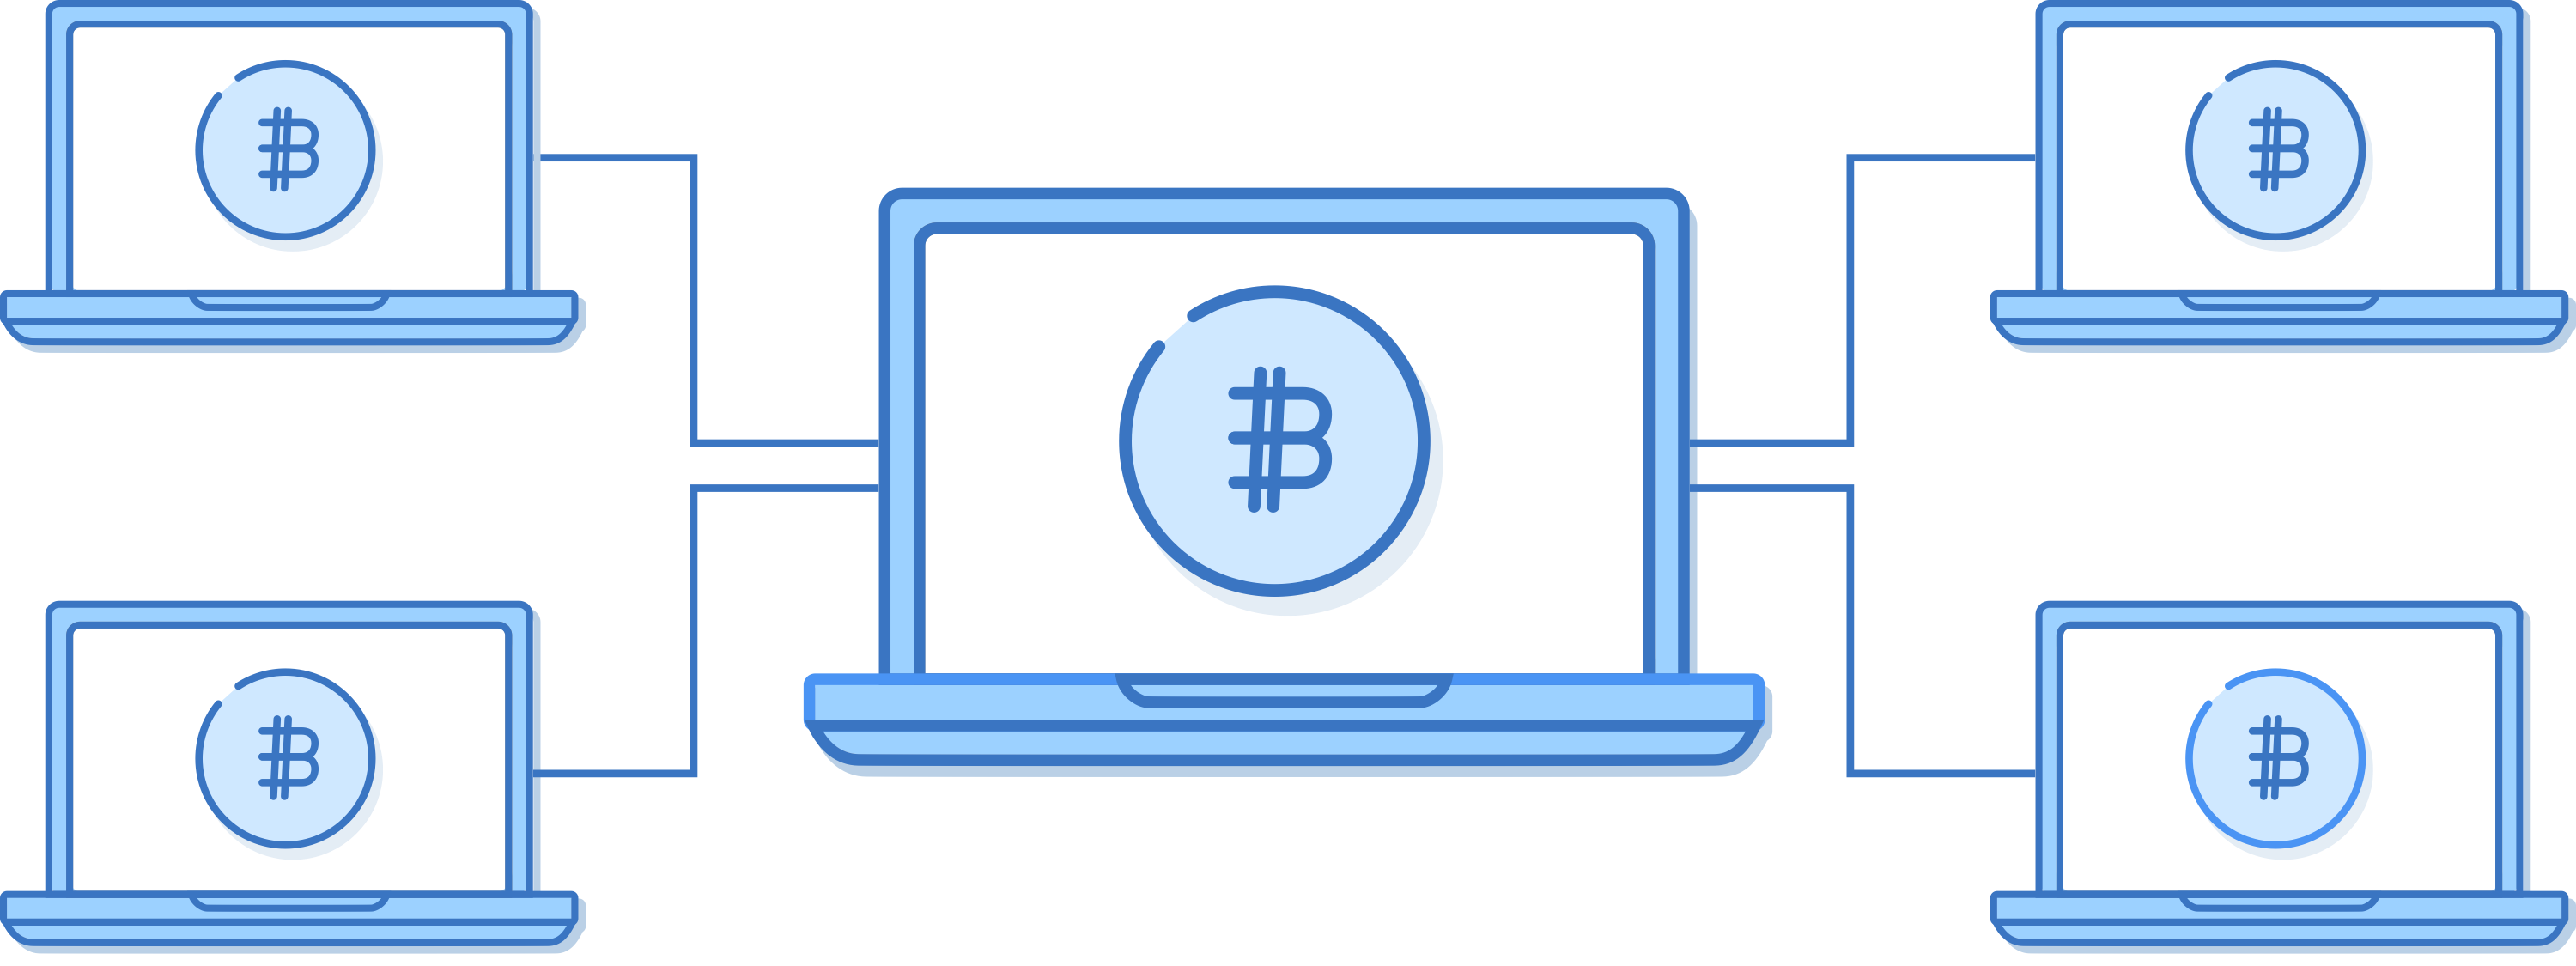
\includegraphics[width=\textwidth]{images/fig1.png}
    \caption{\footnotesize{\textit{Bitcoin is een netwerk van computers die de bitcoinclientsoftware draaien}.}}
    \label{fig1}
\end{figure}

\noindent Later in het boek komen we terug op de motivaties achter bitcoin.

\section{Waar komt bitcoin vandaan?}

Bitcoin is rond 2008 uitgevonden door een of meer personen die bekend staan onder het pseudoniem  \href{https://nl.wikipedia.org/wiki/Satoshi_Nakamoto}{\textbf{Satoshi Nakamoto}}\footnote{Door de gemeenschap wordt gerefereerd aan Satoshi als man. In dit boek zullen we ook als dusdanig naar hem refereren ondanks dat het onbekend is of het gaat om een man, vrouw of groep personen}. Niemand kent de identiteit van Satoshi, en voor zover we weten is hij verdwenen en heeft hij al jaren niets meer van zich laten horen.

Op 11 februari 2009 berichtte Satoshi over een vroege versie van bitcoin op een online forum voor mensen die werken aan cryptografie en veel waarde hechten aan individuele privacy en vrijheid --- \textit{cypherpunks}. Hoewel dit niet de eerste officiële aankondiging van bitcoin was, bevatte het een goede samenvatting van Satoshi's beweegredenen. Daarom gebruik ik het om de basis te leggen voor onze discussie.

Ik zal een aantal citaten weergeven die verduidelijken welke problemen van het huidige financiële systeem Satoshi probeerde op te lossen:

\begin{quotation}
Ik heb een nieuw open source P2P e-cash systeem ontwikkeld genaamd bitcoin. Het is volledig gedecentraliseerd, zonder centrale server of vertrouwde partijen. Alles is gebaseerd op cryptografisch bewijs in plaats van vertrouwen. [...]

Het kernprobleem met conventionele valuta is het vertrouwen dat nodig is om het te laten werken. De centrale bank moet worden vertrouwd, maar de geschiedenis van fiatvaluta zit vol met schendingen van dat vertrouwen. We moeten banken vertrouwen om ons geld te bewaren en elektronisch over te maken, maar ze lenen het uit in golven van kredietbubbels met nauwelijks een fractie van die waarde in reserve. We moeten hen onze privacy toevertrouwen, en we moeten erop vertrouwen dat ze identiteitsdieven weerhouden om onze rekeningen te plunderen. Hun enorme overheadkosten maken microbetalingen onmogelijk.

Vroeger hadden \textquotedbl{}multi-user time-sharing computersystemen\textquotedbl{} een vergelijkbaar probleem. Voor sterke encryptie moesten gebruikers nog vertrouwen op wachtwoorden om hun bestanden te beveiligen [...]

Toen werd sterke encryptie beschikbaar voor de massa en was vertrouwen niet langer nodig. Gegevens konden worden beveiligd waardoor het voor anderen onmogelijk was om toegang te krijgen, ongeacht om welke reden, ongeacht hoe goed het excuus, wat er ook gebeurt.

Het wordt tijd dat we dit ook hebben voor geld. Met e-valuta op basis van cryptografisch bewijs, zonder de noodzaak om een externe tussenpersoon te vertrouwen. Geld kan veilig zijn en transacties moeiteloos. [...]

De oplossing van bitcoin is om een peer-to-peer-netwerk te gebruiken om te controleren op dubbele uitgaven. In een notendop werkt het netwerk als een gedistribueerde tijdstempel, waarbij de eerste uitgave van een munt van een tijdstempel wordt voorzien. Het maakt gebruik van het feit dat informatie gemakkelijk te verspreiden is, maar moeilijk is om tegen te houden.

Voor meer informatie over hoe het werkt, zie het ontwerpdocument op \href{http://www.bitcoin.org/bitcoin.pdf}{http://www.bitcoin.org/bitcoin.pdf}.\footnote{Kijk voor de Nederlandse versie van de whitepaper op: \href{https://btcdirect.eu/nl-nl/bitcoin-whitepaper}{https://btcdirect.eu/nl-nl/bitcoin-whitepaper}}
\par\raggedleft--- \textup{SATOSHI NAKAMOTO}
\end{quotation}

\section{Welke problemen lost het op?}

Laten we een aantal van Satoshi's beweringen nader onderzoeken. Doorheen het boek zullen we bespreken hoe deze concepten daadwerkelijk worden geïmplementeerd. Maak je geen zorgen als iets onbekend aanvoelt in deze sectie want we gaan er later dieper op in. Het idee is om de bedoeling van Satoshi te begrijpen, zodat we ze later in dit boek kunnen onderzoeken.

\begin{quote}
\textit{Ik heb een nieuw open source P2P e-cash systeem ontwikkeld}
\end{quote}

P2P staat voor \textit{peer-to-peer} en geeft een systeem aan waarbij één persoon een interactie heeft met een ander, zonder tussenpartij. De twee partijen (ontvanger en verzender) zijn gelijkwaardig. Je herinnert je misschien P2P-technologieën zoals Napster, Kazaa en BitTorrent, waarmee mensen voor het eerst met elkaar bestanden, muziek en films konden delen zonder tussenpersoon. Satoshi ontwierp bitcoin om mensen de mogelijkheid te geven om op vrijwel dezelfde manier elektronisch contant geld (\textit{e-cash}) uit te wisselen zonder tussenpersoon.

De software is \textit{open source}, wat betekent dat iedereen kan zien hoe het werkt en iedereen kan bijdragen. Dit is belangrijk omdat het zorgt voor transparantie. Er is geen vertrouwen nodig. We hoeven niets te geloven van wat Satoshi schreef in zijn berichten over hoe de software werkt. We kunnen de code bekijken en controleren hoe het werkt. Bovendien kunnen we de functionaliteit van het systeem verbeteren door de code te wijzigen.

\begin{quote}
\textit{Het is volledig gedecentraliseerd, zonder centrale server of vertrouwde partijen...}
\end{quote}

Satoshi vermeldt dat het systeem \textit{gedecentraliseerd} is om het te onderscheiden van systemen die wel centrale aansturing hebben. Eerdere pogingen om digitaal contant geld te creëren, zoals DigiCash van David Chaum, werden ondersteund door een \textit{centrale server}; een computer of set van computers die verantwoordelijk waren voor uitgifte en verificatie van betalingen, onder controle van één bedrijf.

Dergelijke centraal aangestuurde particuliere vormen van digitaal geld zijn gedoemd te mislukken; we kunnen niet vertrouwen op geld dat kan verdwijnen wanneer een bedrijf failliet gaat, wordt gehackt, last heeft van IT-problemen of wordt gestopt door de overheid.

Bitcoin, aan de andere kant, wordt niet gerund en gecontroleerd door een enkel bedrijf, maar door een netwerk van individuen en bedrijven van over de hele wereld. Het stoppen van bitcoin vereist het stoppen van tienduizenden tot honderdduizenden computers over de hele wereld, waarvan velen lastig te traceren zijn. Het is een hopeloos kat-en-muisspel aangezien elke aanval van deze aard eenvoudigweg de creatie van nieuwe \textit{bitcoin-nodes} of computers op het netwerk aanmoedigt.

\begin{quote}
\textit{ ... alles is gebaseerd op cryptografisch bewijs in plaats van vertrouwen}
\end{quote}

Het internet en de meeste moderne computersystemen zijn gebouwd op cryptografie; een methode om informatie te versleutelen zodat alleen de ontvanger van de informatie deze kan ontcijferen. Hoe ontsnapt bitcoin aan de noodzaak van \textit{vertrouwen}? We zullen hier later in het boek op ingaan, maar het basisidee is dat in plaats van iemand te vertrouwen die zegt \textquotedbl{}Ik ben Alice\textquotedbl{} of \textquotedbl{}Ik heb \$10 in mijn account\textquotedbl{}, we cryptografie kunnen gebruiken om dezelfde feiten dusdanig te presenteren zodat de ontvanger van het bericht dit eenvoudig zelf kan verifiëren en het onmogelijk is om te vervalsen. Bitcoin maakt gebruik van cryptografie om deelnemers in staat te stellen het gedrag van alle anderen te controleren, zonder dat hierbij een centrale partij vertrouwt hoeft te worden.

\begin{quote}
\textit{We moeten hen [de banken] onze privacy toevertrouwen, en we moeten erop vertrouwen dat ze identiteitsdieven ervan weerhouden om onze rekeningen te plunderen}
\end{quote}

In tegenstelling tot het gebruik van een bankrekening, het digitale betalingssysteem of kredietkaarten, stelt bitcoin twee partijen in staat om transacties uit te voeren zonder persoonlijke identificatie op te geven. Banken, kredietkaartmaatschappijen, betalingsverwerkers en overheden beschikken over gecentraliseerde databanken van consumentengegevens. Deze gegevens zijn een gigantische buit voor hackers. Zo werden bij de hack van Equifax in 2017 de identiteits- en financiële gegevens van meer dan 140 miljoen mensen buitgemaakt. Dit soort databanken en de bijbehorende hacks kunnen resulteren in identiteitsfraude op grote schaal. 

Bitcoin ontkoppelt financiële transacties van identiteiten uit de echte wereld. Immers, wanneer we contant geld aan iemand geven, hoeft de ontvanger niet te weten wie we zijn en hoeft de betaler zich geen zorgen te maken dat zijn informatie wordt gebruikt om hem op een later moment te bestelen. Waarom zouden we niet hetzelfde, of meer, verwachten van digitaal geld?

\begin{quote}
\textit{De centrale bank moet worden vertrouwd om de valuta niet te devalueren, maar de geschiedenis van fiatvaluta zit vol met schendingen van dat vertrouwen}
\end{quote}

\textit{Fiat}, Latijn voor \textquotedbl{}laat het gebeuren\textquotedbl{}, verwijst naar valuta uitgegeven door de overheid en centrale bank en dat door de overheid als wettig betaalmiddel is aangenomen. Historisch gezien werd geld gemaakt uit dingen die moeilijk zijn om te produceren, gemakkelijk zijn om te verifiëren en gemakkelijk zijn om te vervoeren, zoals schelpen, glaskralen, zilver en goud. Telkens wanneer iets als geld werd gebruikt, bestond de verleiding om er meer van te maken. Als iemand langskwam met superieure technologie om snel veel van iets te creëren, verloor het goed zijn waarde. Zo konden Europese kolonisten het Afrikaans continent ontdoen van haar rijkdom, door te handelen in glazen kralen die voor de Europeanen gemakkelijk, maar voor de Afrikanen moeilijk, te produceren waren. Dit is waarom goud al zo lang wordt beschouwd als betrouwbare vorm van geld - het is moeilijk om snel meer goud te produceren.\footnote{Voor een goed overzicht van de monetaire geschiedenis raad ik het essay \textit{Shelling Out} van Nick Szabo aan: \href{https://nakamotoinstitute.org/shelling-out}{https://nakamotoinstitute.org/shelling-out}}

We zijn langzaam overgestapt van een wereldeconomie met goud als geld naar een wereld waarbij papieren certificaten werden uitgegeven als claim op datzelfde goud. Uiteindelijk werden door president Nixon de papieren claims volledig losgekoppeld van goud. Hij maakte in 1971 een einde aan de internationale inwisselbaarheid van de Amerikaanse dollar voor goud.

Het einde van de goudstandaard stelde overheden en centrale banken in staat om de geldhoeveelheid naar believen te vergroten, waardoor ieder biljet in omloop minder waard werd. Dit staat bekend als \textit{geldontwaarding}. Hoewel fiatvaluta wordt uitgegeven door een regering, het inwisselbaar is voor niets, en we het allemaal dagelijks gebruiken, is het eigenlijk een relatief nieuw experiment in de wereldgeschiedenis.

We moeten erop vertrouwen dat onze overheden de drukpers niet misbruiken, maar ver hoeven we niet te zoeken om voorbeelden van schendingen van dat vertrouwen te vinden. Dit zien we voornamelijk terug in autocratische regimes, waar de overheid directe invloed op de geldpers heeft. Een bekend voorbeeld is Venezuela, waar de munt nagenoeg waardeloos is geworden. De Venezolaanse bolivar ging van een koers van 2 bolivar per Amerikaanse dollar in 2009 naar 250.000 bolivar per Amerikaanse dollar in 2019. Terwijl ik dit boek schrijf, is de ineenstorting van Venezuela volop aan de gang als gevolg van het vreselijke economische wanbeleid van de regering.

Satoshi wilde een alternatief bieden voor \textit{fiatvaluta} waarvan het aantal te allen tijde onvoorspelbaar kan worden verhoogd. Om \textit{ontwaarding} te voorkomen, ontwierp Satoshi een geldsysteem waarbij het totale aanbod vooraf werd vastgelegd en het uitgeven van nieuwe munten een voorspelbaar en onveranderlijk patroon volgt. Er zullen slechts 21 miljoen bitcoins bestaan en elke bitcoin kan worden verdeeld in 100 miljoen eenheden die nu satoshis worden genoemd. In de code is vastgelegd dat rond het jaar 2140 het eindtotaal wordt bereikt van 2,1 biljard satoshis.

Tot bitcoin was het onmogelijk om te verkomen dat een digitaal goed oneindig werd gekopieerd. Het is goedkoop en gemakkelijk om een digitaal boek, audio- of video-bestand digitaal te kopiëren en door te sturen. De enige uitzonderingen hierop waren digitale goederen die beheerd werden door tussenpersonen. Bijvoorbeeld wanneer je een film kijkt via Netflix, dan kun je deze alleen op jouw apparaat bekijken omdat Netflix de film levert. Je kan deze film zelf niet verspreiden of kopiëren. Op dezelfde manier wordt je digitale geld beheerd door de bank. Het is de taak van de bank om bij te houden hoeveel geld je hebt, en als je het aan iemand anders overdraagt, regelt de bank de overdracht.\footnote{Ze zijn dus ook in staat deze te weigeren}

Bitcoin is het eerste digitale systeem dat schaarste afdwingt zonder tussenpersonen en het is het eerste goed waarvan het totale aanbod en het uitgifteschema vooraf bekend is. Zelfs edelmetalen zoals goud hebben deze eigenschap niet, omdat we meer goud kunnen delven als het rendabel is om dat te doen. Stel je voor dat je een asteroïde ontdekt die tien keer zoveel goud bevat als wij op aarde hebben. Wat zou er gebeuren met de prijs van goud? Bitcoin is immuun voor dergelijke ontdekkingen. Het is onmogelijk om er meer van te produceren, en we zullen in latere hoofdstukken uitleggen waarom.
 
De aard van geld en de werking van het bestaande monetaire systeem zijn ingewikkeld. Dit boek gaat hier niet dieper op in. Als je hier meer over wilt weten in de context van bitcoin, dan raad ik \textit{De Bitcoin Standaard} van Saifedean Ammous aan.

\begin{quote}
\textit{Gegevens konden worden beveiligd op een manier waardoor het voor anderen onmogelijk was om toegang te krijgen, ongeacht om welke reden, ongeacht hoe goed het excuus, wat er ook gebeurt. [...]
Het wordt tijd dat we dit ook hebben voor geld.} 
\end{quote}

Onze huidige systemen om geld veilig te stellen, zoals het op de bank zetten, vertrouwen erop dat iemand anders zijn werk goed doet. Vertrouwen op zo'n tussenpersoon vereist niet alleen vertrouwen dat ze niets kwaadaardigs of dwaas zullen doen, maar ook vertrouwen dat de overheid niet via druk op de tussenpersoon dergelijke dingen doet. Denk hierbij aan zaken als iemand de toegang tot hun geld ontzeggen of het geld onteigenen. Helaas is keer op keer aangetoond dat overheden wanneer zij bedreiging verwachten of zien, dit soort dingen kunnen doen en tot uitvoering brengen.

Het klinkt misschien gek voor iemand die in de Verenigde Staten woont (of in een andere sterk gereguleerde economie) om te denken dat je op een dag wakker kan worden en dat dan al je geld weg is, maar het gebeurt de hele tijd. Ik heb zelf eens voorgehad dat mijn tegoed op Paypal bevroren was omdat ik mijn account al maanden niet had gebruikt. Het kostte me meer dan een week om weer toegang te krijgen tot \textquotedbl{}mijn\textquotedbl{} geld. Ik heb het geluk dat ik in de Verenigde Staten woon, waar ik tenminste juridische hulp kan zoeken als PayPal mijn tegoed bevriest, en waar ik er in principe op vertrouw dat mijn regering en de bank mijn geld niet zullen stelen.

Er zijn veel ergere dingen gebeurd en nog steeds aan de orde in landen met minder vrijheid, zoals banken die sluiten tijdens de crisis in Griekenland (2015)\footnote{\href{https://www.nbcnews.com/business/business-news/greece-crisis-banks-shut-week-restrictions-imposed-atms-n383606}{https://nbcnews.com/business/business-news/greece-crisis-banks-shut-week-restrictions-imposed-atms-n383606}}, banken in Cyprus die via bail-ins het geld van hun klanten in beslag nemen (2013), of de overheid die bepaalde bankbiljetten waardeloos verklaart in India (2016)\footnote{\href{https://www.washingtonpost.com/world/asia\_pacific/india-invalidates-large-bank-notes-in-crackdown-on-crime/2016/11/08/cc705ee2-a5c6-11e6-ba46-53db57f0e351\_story.html}{https://www.washingtonpost.com/world/asia\_pacific/india-invalidates-large-bank-notes-in-crackdown-on-crime/2016/11/08/cc705ee2-a5c6-11e6-ba46-53db57f0e351\_story.html}}.

Ik ben opgegroeid in de voormalige Sovjet-Unie. Daar reguleerde de overheid de economie, wat leidde tot enorme tekorten aan goederen. Het was illegaal om vreemde valuta zoals de Amerikaanse dollar te bezitten. Toen mijn ouders weg wilden, konden we slechts een beperkt bedrag per persoon naar dollars omwisselen. De wisselkoers was door de overheid bepaald en ver verwijderd van de wisselkoers op de vrije markt. In feite heeft de regering ons het kleine beetje vermogen dat we hadden ontnomen, door een ijzeren greep te houden op de economie en het betalingsverkeer.

Autocratische landen hebben de neiging om strenge economische controles in te voeren om te voorkomen dat mensen hun geld uit banken opnemen, het land uitvoeren of inruilen voor nog-niet-waardeloze valuta zoals de Amerikaanse dollar. Hierdoor heeft de regering vrij spel om krankzinnige economische experimenten, zoals het socialistische systeem van de Sovjet-Unie, uit te voeren.

Bitcoin werkt niet op basis van vertrouwen in een derde partij voor het veilig stellen van je geld. In plaats daarvan maakt bitcoin het \textit{onmogelijk} voor anderen om toegang te krijgen zonder een speciale sleutel die alleen de eigenaar bezit, \textit{ongeacht om welke reden, ongeacht hoe goed het excuus, wat er ook gebeurt}. Door bitcoin te bezitten, bezit je de sleutels van je eigen financiële vrijheid. Bitcoin scheidt geld en staat.

\begin{quote}
\textit{De oplossing van bitcoin is om een peer-to-peer-netwerk te gebruiken om te controleren op dubbele uitgaven [...] als een gedistribueerde tijdstempel, waarbij de eerste uitgave van een munt van een tijdstempel wordt voorzien.}
\end{quote}

Een \textit{netwerk} verwijst naar het idee dat een stel computers zijn verbonden en informatie naar elkaar kunnen sturen. Het woord \textit{gedistribueerd} betekent dat er geen centrale partij aan de macht is, maar dat alle deelnemers samenwerken om het netwerk succesvol te maken.

In een systeem zonder centrale controle is het belangrijk dat niemand vals kan spelen. Het idee van \textit{dubbele uitgaven} verwijst naar de mogelijkheid om twee keer hetzelfde geld uit te geven. Dit is geen probleem met fysiek geld, want het geld wisselt van hand zodra je het uitgeeft. Digitale transacties kunnen echter worden gekopieerd, net als muziek of films. Wanneer je geld overmaakt via een bank, zorgt de bank ervoor dat je niet twee keer hetzelfde geld kunt verplaatsen. In een systeem zonder centrale controle, hebben we een manier nodig om dit soort \textit{dubbele uitgaven} te voorkomen (Dubbele uitgaven zijn in feite hetzelfde als geld vervalsen). 

Satoshi beschrijft dat de deelnemers van het bitcoinnetwerk samenwerken om transacties van \textit{tijdstempels} te voorzien. Door deze tijdstempel weten we welke transactie eerst kwam zodat we toekomstige pogingen om datzelfde geld uit te geven afwijzen. In de volgende hoofdstukken zullen we dit systeem vanaf de basis bespreken. Het zal ons in staat stellen om vals spel te detecteren zonder te vertrouwen op een centrale uitgever of validator.


Bitcoin was geen uitvinding die op zichzelf stond. In de paper noemde Satoshi verschillende belangrijke pogingen om soortgelijke systemen te implementeren, waaronder Wei Dai's b-money en Adam Back's Hashcash. Ondanks de technologische inzichten van voorgangers, had nog niemand de juiste oplossing gevonden. Maar de uitvinding van bitcoin bracht daar verandering in, waardoor het eerste systeem voor de uitgifte en het overmaken van een echt schaars, digitaal geld zonder centrale controle mogelijk werd.

Satoshi loste een aantal interessante technische problemen op om de kwesties van privacy, ontwaarding en centrale controle in de huidige monetaire stelsels aan te pakken:

\begin{enumerate}
    \item Hoe zet je een peer-to-peer-netwerk op, waar iedereen vrijwillig aan kan deelnemen.
    \item Hoe koppel je een groep mensen zodat zij gezamenlijk een grootboek bij kunnen houden, zonder hun identiteit te onthullen en zonder dat zij elkaar hoeven te vertrouwen, zelfs als sommigen van hen oneerlijk zijn.
    \item Hoe stel je mensen in staat om hun eigen, onvervalsbare valuta uit te geven, zonder op een centrale uitgever te steunen om de schaarste te verzekeren.
\end{enumerate}

Toen bitcoin van start ging, gebruikte slechts een handvol mensen het en draaiden zij de bitcoin-software op hun \textit{nodes} (computers, we gaan hier later verder op in). De meeste mensen dachten destijds dat het een grap was, of dat het systeem na verloop van tijd ernstige ontwerpfouten zou bevatten waardoor het zou falen.

Maar steeds meer mensen sloten zich aan bij het netwerk. Ze beveiligden het netwerk met hun computers, ruilden hun valuta in voor bitcoin, of accepteerden bitcoin in ruil voor goederen of diensten. Dit alles verstevigde de gedachte dat bitcoin waarde had. Vandaag, tien jaar later, wordt bitcoin gebruikt door miljoenen mensen en draaien tienduizenden tot honderdduizenden nodes de gratis bitcoin software, ontwikkelt door honderden vrijwilligers en bedrijven wereldwijd.

Laten we onderzoeken hoe we zo'n systeem kunnen bouwen!




\hypertarget{chap2}{%
\chapter{De tussenpersoon verwijderen}\label{chap2}}

In het vorige hoofdstuk hebben we besproken dat bitcoin een peer-to-peer systeem is voor de overdracht van waarde. Voordat we ingaan op hoe dat werkt, kijken we eerst hoe een traditionele bank of betalingsverwerker omgaat met het beheer van eigendom en overdrachten van activa.

\section{Banken zijn slechts grootboeken}

Hoe werkt een digitale betaling via de bank, PayPal of ApplePay? Heel eenvoudig, fungeren deze tussenpersonen als veredelde grootboeken van rekeningen en overschrijvingen.

Het doel van een bank is om tegoeden op te slaan en te bewaken. Maar tegoeden zijn tegenwoordig voornamelijk elektronisch, in plaats van munten of papier. Als zodanig is het nu de taak van een bank om data te beheren en te bewaken. Omdat de gegevens elektronisch zijn, is de beveiliging ook voornamelijk elektronisch. Banken maken gebruik van softwarematige inbraakdetectiesystemen, back-ups om te beschermen tegen gegevensverlies, audits door derden om er zeker van te zijn dat interne processen niet in het gedrang komen en ze verzekeren zich uit voorzorg voor het geval er iets misgaat.

Hieronder zie je hoe banken werken. In dit voorbeeld hebben we het over een bank, maar je kan dit lezen als elke partij die betalingen verwerkt. We beginnen met een grootboek van rekeningen waaruit blijkt dat Alice en Bob geld hebben gestort bij de bank.

\begin{alltt}
\underline{Grootboek van de bank}

    1. Alice: Credit voor cash storting +2€
    2. Bob: Credit voor cash storting +10€
\end{alltt}

Wanneer Alice €2 naar Bob wil sturen, belt ze haar bank of gebruikt ze een website of mobiele app van haar bank, logt ze in bij de bank met behulp van een gebruikersnaam en wachtwoord of pincode, en doet vervolgens het verzoek tot overdracht. De bank registreert dit in hun grootboek.

\begin{alltt}
\underline{Grootboek van de bank}

    1. Alice: Credit voor cash storting +€2
    2. Bob: Credit voor cash storting +10€
    3. Alice: Debet -2€
    4. Bob: Credit +2€
\end{alltt}

De bank heeft de credits en debets en bijbehorende tegoeden geregistreerd, en nu is het geld overgedragen.

\section{Het dubbele-uitgavenprobleem}

Wat gebeurt er als Alice diezelfde twee dollar nu weer probeert uit te geven? Dit wordt het \textit{dubbele-uitgavenprobleem} genoemd. Zij dient het verzoek in bij de bank, maar de bank zegt: "Sorry, we zien dat je die €2 al hebt uitgegeven aan Bob. Je kan dat geld niet meer uitgeven."

Wanneer je een centrale autoriteit hebt zoals een bank, is het heel gemakkelijk voor de bank om te zien dat je probeert geld uit te geven dat je al hebt uitgegeven. Dat komt omdat zij de enigen zijn die het grootboek kunnen wijzigen. Zij beschikken over verschillende interne processen zoals back-ups en audits, om ervoor te zorgen dat het grootboek correct is en om te zorgen dat er niet mee wordt geknoeid.

We noemen dit een \textit{gecentraliseerd} systeem omdat het een enkel controlepunt heeft.

\begin{figure}
    \centering
    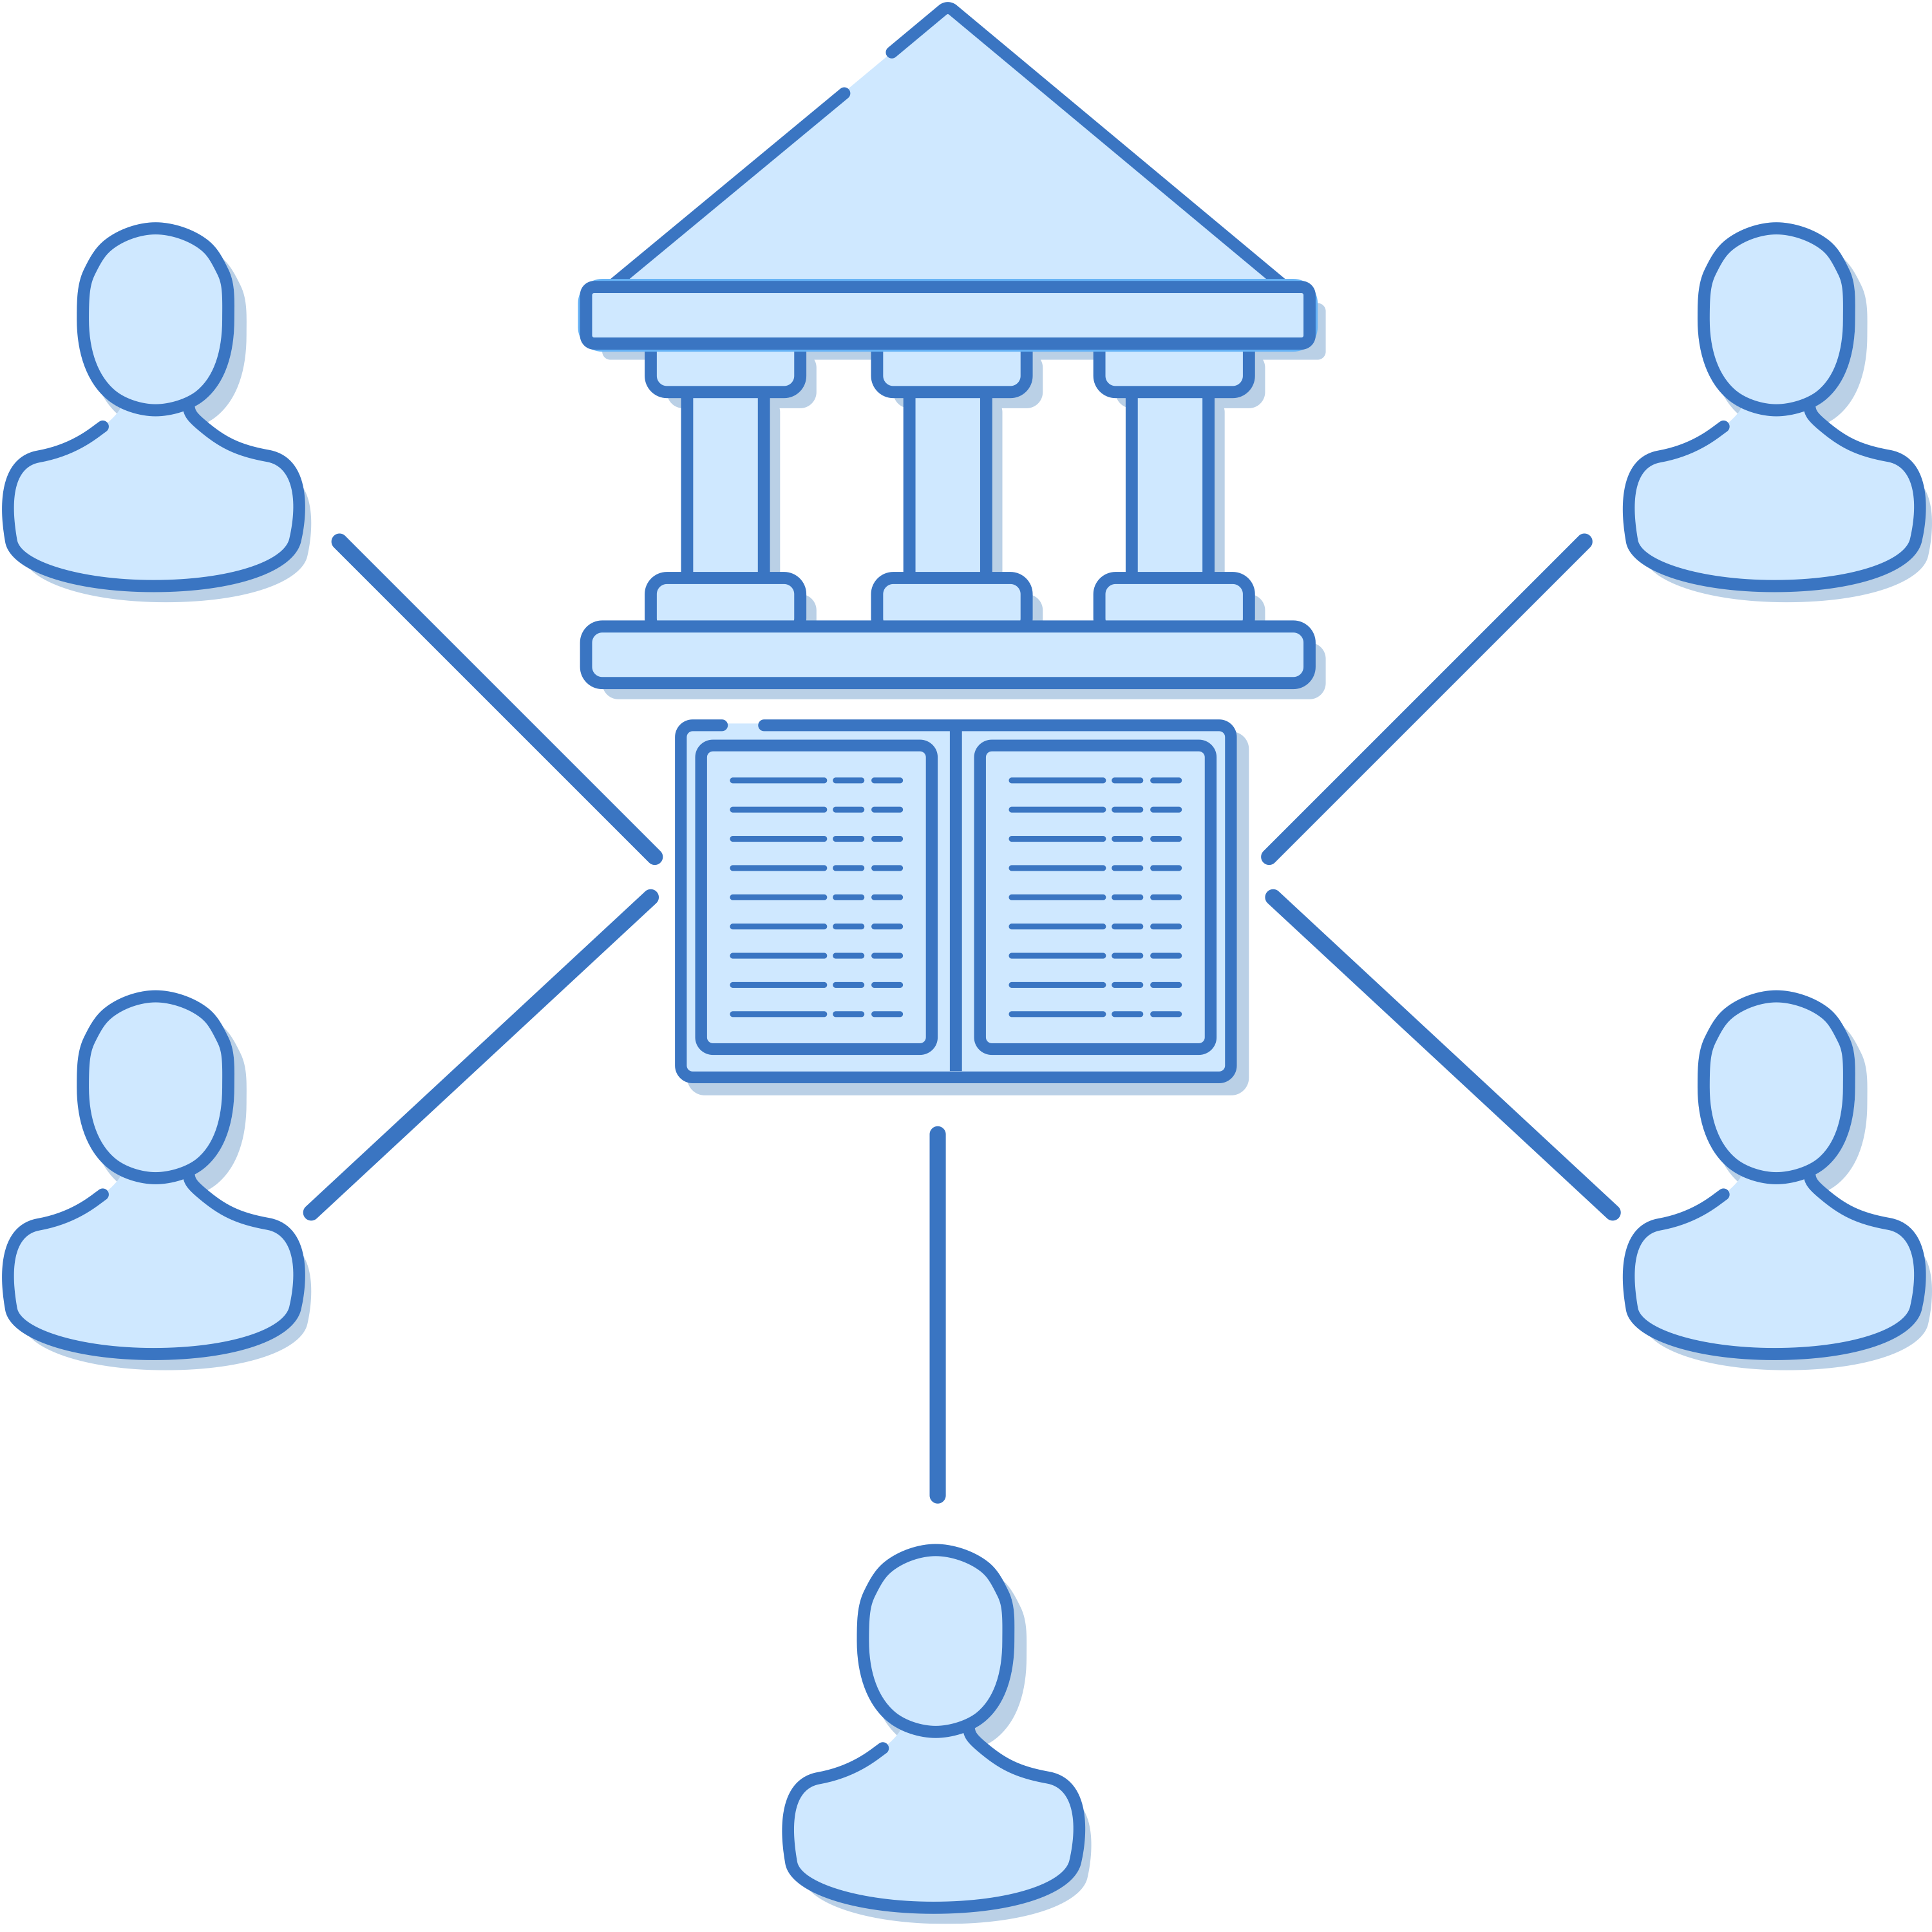
\includegraphics[width=0.6\textwidth]{images/fig2.png}
    \caption{\footnotesize{\textit{De bank houdt een grootboek bij waar iedereen toegang toe heeft, maar alleen via de bank bij kan.}}}
    \label{fig2}
\end{figure}

\section{Het grootboek delen tussen verschillende partijen}

Het eerste probleem dat bitcoin wil oplossen, is het verwijderen van een tussenpersoon door het creëren van een \textit{peer-to-peer} systeem. Stel je voor dat banken verdwenen zijn en we ons financiële systeem opnieuw moeten creëren. Hoe kunnen we een grootboek bijhouden zonder centrale partij?

Als we niet één centraal grootboek hebben, moet het zo zijn dat het grootboek van het volk is. \textit{Vive la révolution}. Dit is hoe we dat doen.

Eerst komen een aantal mensen samen en creëren zij een \textit{netwerk}. Dit betekent simpelweg dat een manier bestaat om informatie met elkaar te delen. Laten we zeggen dat we telefoonnummers of Snapchat-accounts uitwisselen. Wanneer Alice geld wil overmaken naar Bob, belt ze niet naar de bank, maar zegt ze tegen al haar vrienden: \textquotedbl{}Ik stuur €2 naar Bob\textquotedbl{}. Iedereen bevestigt met: \textquotedbl{}Top, we noteren het\textquotedbl{}, en schrijft het in hun eigen kopie van het grootboek. Het ziet er uit zoals in Figuur \ref{fig3}.

\begin{figure}
    \centering
    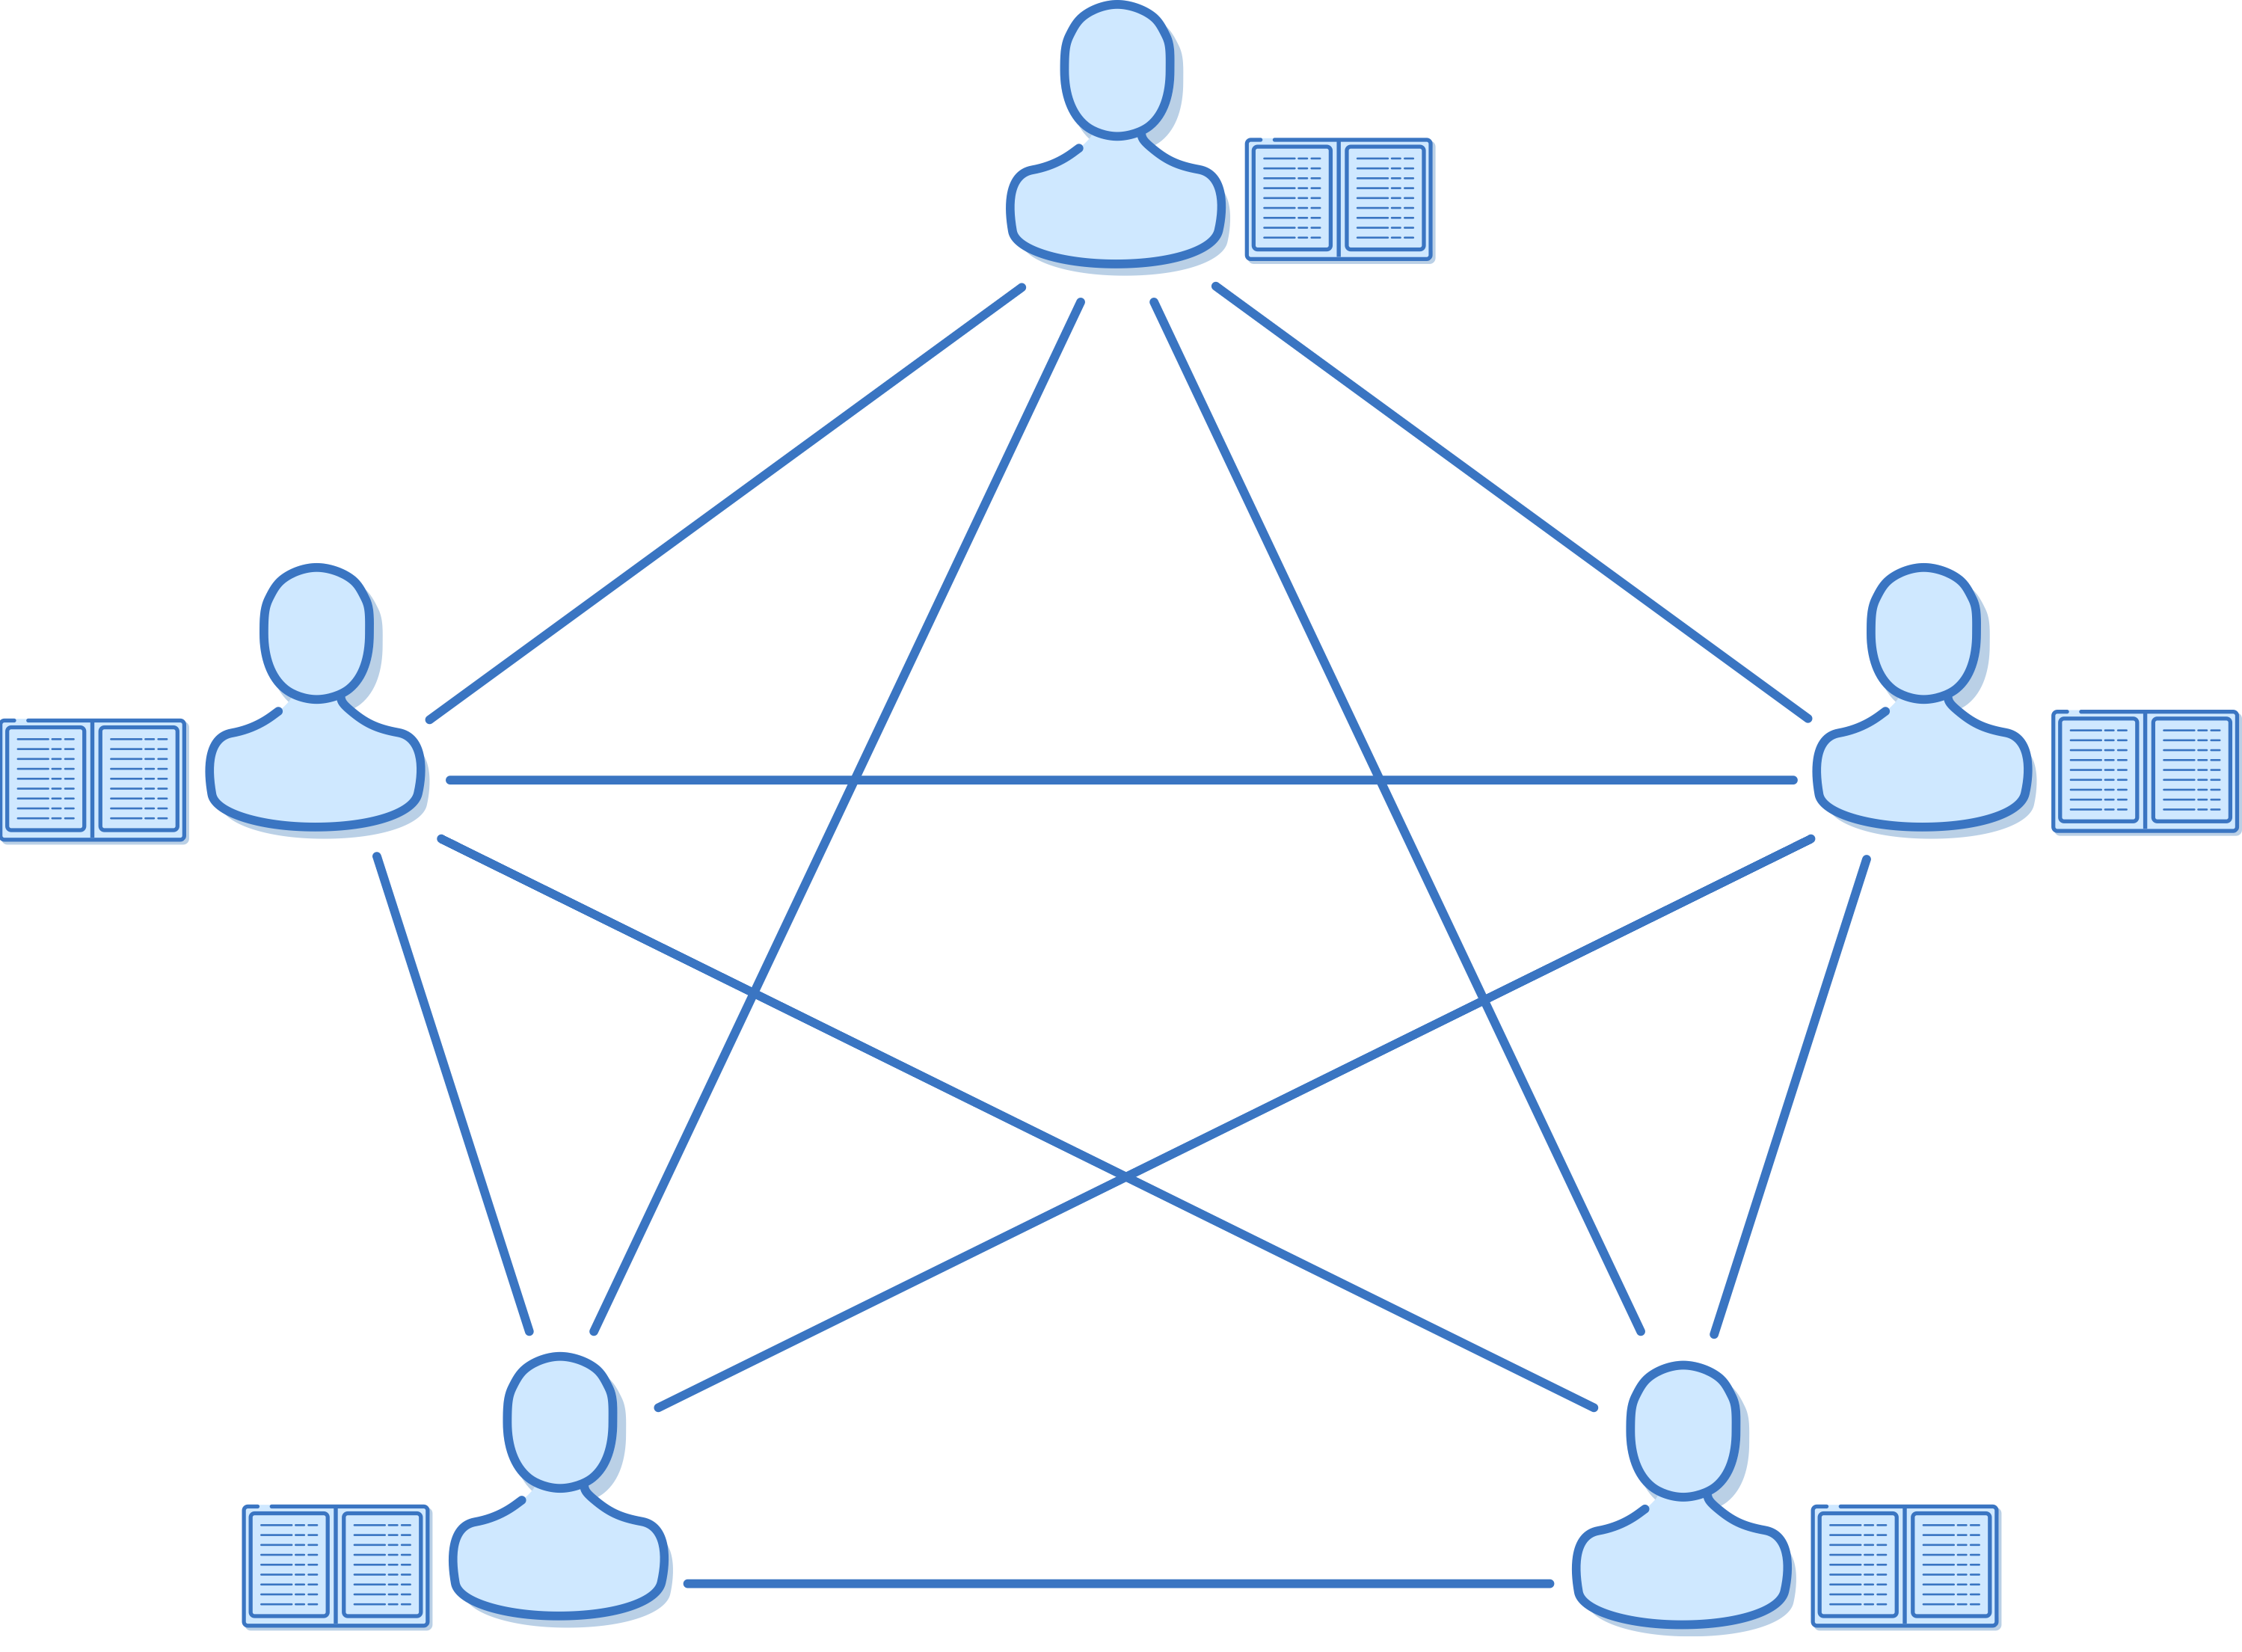
\includegraphics[width=0.6\textwidth]{images/fig3.png}
    \caption{\footnotesize{\textit{Iedereen heeft een eigen kopie van het grootboek, waar ze onafhankelijk van een ander bij kunnen.}}}
    \label{fig3}
\end{figure}

Dus nu heeft iedereen (in plaats van enkel de bank) een kopie van het grootboek in handen. Telkens wanneer iemand geld wil uitgeven, vertellen ze het aan al hun vrienden. Iedereen houdt de transacties bij. Het grootboek staat niet meer op één plek. Dit heet \textit{gedistribueerd}. We noemen we het ook \textit{decentraal}, omdat geen enkele centrale partij het voor het zeggen heeft. Er hoeft geen tussenpersoon meer vertrouwd te worden.


Nu we geen tussenpersoon hebben, hoe gaan we dan om met dubbele uitgaven? Wie of wat kunnen we (in plaats van de bank) raadplegen om na te gaan of het geld dat wordt uitgegeven nog niet is uitgegeven? Omdat iedereen een kopie van het grootboek heeft, moeten we iedereen raadplegen. Het systeem zoals we nu bespreken, is \textit{gebaseerd op consensus} omdat er in het netwerk consensus heerst. Iedereen is het eens over een bepaalde versie van de waarheid.

Als Alice probeert om de €2 die ze al naar Bob heeft gestuurd opnieuw uit te geven, zal haar transactie worden afgewezen door iedereen op het netwerk. De leden op het netwerk zullen hun grootboeken raadplegen en aan Alice vertellen dat het geld al is uitgegeven. Ze zouden haar tweede transactie van diezelfde €2 dus niet opnemen. We hebben nu een peer-to-peer consensusnetwerk voor het registreren van eigendom en overdrachten van tegoeden.

Zolang partijen \textit{toestemming} nodig hebben om deel te mogen nemen aan ons gedistribueerde grootboek, en we erop kunnen \textit{vertrouwen} dat elke partij eerlijk is, werkt het systeem. Maar dit soort ontwerpen kunnen niet geschaald worden om door miljoenen mensen van over de hele wereld te worden gebruikt. Gedistribueerde systemen bestaande uit willekeurige deelnemers zijn inherent onbetrouwbaar. Sommige mensen gaan af en toe offline. Dat betekent dat ze mogelijk niet op de hoogte zijn van onze transacties op het moment dat we die uitsturen. Anderen proberen ons misschien actief te bedriegen door te zeggen dat bepaalde transacties juist wel of niet hebben plaatsgevonden. Nieuwe mensen kunnen zich aansluiten bij het netwerk en zo ontstaan conflicterende kopieën van het grootboek.

In het volgende deel onderzoeken we hoe iemand zou kunnen proberen om vals te spelen.

\section{De dubbele-uitgaven aanval}

Als ik Alice ben, kan ik \textit{samenspannen} met een aantal van de andere mensen en hen vertellen: \textquotedbl{}Als ik geld uitgeef, schrijf het dan niet in jullie grootboek. Doe alsof het nooit gebeurd is.\textquotedbl{} Laten we eens kijken hoe Alice zo'n dubbele-uitgaven aanval kan uitvoeren.

Beginnend met een saldo van €2, doet Alice het volgende:

\begin{enumerate}
    \item Ze stuurt haar €2 naar Bob, om een reep chocolade te kopen. Nu heeft Alice €0 over.
    \item David, Eva en Femke spannen samen met Alice en schrijven de transactie van Alice naar Bob niet in hun grootboeken. In hun exemplaar heeft Alice haar geld nooit uitgegeven en heeft ze nog steeds een saldo van €2.
    \item Charlotte is een eerlijke grootboekhouder. Ze registreert correct de transactie van Alice naar Bob. In haar grootboek heeft Alice €0.
    \item Henri was een week op vakantie en heeft nog nooit van de transactie gehoord. Hij sluit zich aan bij het netwerk en vraagt om een kopie van het grootboek.
    \item Henri krijgt 4 valse kopieën (David, Eva, Femke en Alice) en één eerlijke kopie (Charlotte). Hoe bepaalt hij welke echt is? Zonder beter systeem vertrouwt hij de meerderheid van deelnemers en wordt dus misleidt. Hij neemt aan dat het nep-grootboek klopt.
    \item Alice koopt een chocoladereep van Henri met de €2 die ze eigenlijk niet heeft. Henri accepteert het omdat voor zo ver hij weet, Alice nog steeds €2 op haar rekening heeft.
    \item Alice heeft nu 2 chocoladerepen en er is €4 aan nepgeld gemaakt in het systeem. Ze betaalt haar vrienden met chocoladerepen, en ze herhalen de aanval 100 keer op elke nieuwe persoon die lid wordt van het netwerk.
    \item Alice heeft nu alle chocoladerepen en alle anderen hebben grote zakken nepgeld gekregen.
    \item Wanneer de verkopers van chocoladerepen het geld willen uitgeven dat Alice ze heeft gestuurd zullen Alice, David, Eva en Femke (die de meerderheid van de netwerk uitmaken) deze uitgaven afwijzen omdat ze weten dat het nepgeld is.
\end{enumerate}

Dit wordt een \textit{consensusfout} genoemd. De mensen in het netwerk kwamen niet tot consensus over de stand van zaken. Doordat er geen beter systeem voor handen was, werd de meerderheidsregel gehanteerd, wat er voor zorgde dat oneerlijke mensen het netwerk konden bedotten en geld konden uitgeven dat ze eigenlijk niet hadden.

Als we een systeem willen maken dat \textit{zonder toestemming} werkt, waar iedereen aan kan deelnemen zonder iemand permissie te moeten vragen, dan moet het weerbaar zijn tegen oneerlijke deelnemers.

\section{Het oplossen van het gedistribueerd consensus probleem}

Nu komen we bij een van de moeilijkste problemen in de technologie: consensus delen tussen partijen waar sommige oneerlijk of onbetrouwbaar zijn. Dit probleem staat bekend als \textit{het probleem van de Byzantijnse Generalen} en de oplossing bleek de sleutel tot succes van Satoshi Nakamoto's ontdekking. Een heleboel mensen moeten het eens worden over de transacties in het grootboek zonder te weten welke grootboekhouders alle transacties correct en eerlijk hebben opgeschreven.

Een naïeve oplossing is simpelweg het aanstellen van eerlijke grootboekhouders. In plaats van iedereen het grootboek laten bijhouden, kiezen we een handvol vrienden zoals Charlotte, Geert, Frank en Zoe om het te doen, omdat ze geen leugens vertellen en iedereen weet dat ze nooit feesten in het weekend.

Dus telkens we een transactie willen verwerken, bellen we Charlotte en de rest op. Ze zijn blij om het grootboek voor ons bij te houden en vragen slechts een kleine vergoeding. Nadat zij de transactie in het grootboek hebben geschreven, bellen ze de anderen om ze op de hoogte te brengen van de wijziging, waarna ook zij die aan het grootboek toevoegen als back-up. 

Dit systeem werkt heel goed, tot op een dag agenten willen weten wie dit schaduw financiële systeem draaiende houdt. Ze arresteren Charlotte, Geert, Frank en Zoe en nemen hen mee, waardoor een einde komt aan ons gedistribueerde grootboek. We hebben allemaal verschillende back-ups, kunnen elkaar niet vertrouwen en kunnen niet achterhalen wiens back-up moet worden gebruikt om een nieuw systeem te starten.

In plaats van een volledige sluiting, zou de overheid onze grootboekhouders ook stilletjes met gevangenisstraffen kunnen bedreigen als ze transacties naar Alice accepteren (die verdacht wordt van het verkopen van drugs). Het systeem is nu effectief onder centrale controle en we kunnen het niet langer \textquotedbl{permissieloos} noemen. 

Wat als we democratie proberen? Laten we een groep van 50 eerlijke mensen zoeken en we houden dagelijks verkiezingen om te bepalen wie die dag het grootboek bij mag houden. Iedereen in het netwerk krijgt een stem.

Dit systeem werkt geweldig totdat mensen geweld of financiële dwang gebruiken om dezelfde doelen te bereiken als voorheen:

\begin{enumerate}
    \item Dwing het electoraat om te stemmen op de grootboekhouders van hun keuze.
    \item Dwing de gekozen grootboekhouders om valse vermeldingen in het grootboek te verwerken of juist bepaalde transacties tegen te houden.
\end{enumerate}

We hebben een probleem. Telkens wanneer we specifieke mensen aanstellen om het grootboek bij te houden, moeten we erop vertrouwen dat ze eerlijk handelen. Er is geen enkele manier om hen te verdedigen tegen dwang om oneerlijk te handelen en het grootboek te corrumperen.

\section{Valse identiteit en Sybil-aanvallen}

Tot nu toe hebben we twee mislukte methoden gezien om eerlijkheid te garanderen: de een maakte gebruik van specifieke grootboekhouders en de ander van democratisch gekozen en roterende grootboekhouders. De zwakte van beide systemen is dat het vertrouwen gekoppeld is aan identiteiten uit de reële wereld: er moeten personen worden aangewezen die verantwoordelijk zijn voor het grootboek. Wanneer we een systeem hanteren waar vertrouwen afhankelijk is van identiteit, lopen we kans op een zogeheten \textit{Sybil-aanval}. Dit is eigenlijk een mooie naam voor imitatie. Het houdt in dat iemand zich voordoet als een ander en is vernoemd naar een vrouw met een meervoudige persoonlijkheidsstoornis.

Heb je ooit een rare SMS ontvangen van een van je vrienden, waarna bleek dat zijn telefoon(nummer) was \textit{gehackt}? Als het om miljarden of zelfs biljoenen dollars gaat, zullen mensen allerlei vormen van geweld rechtvaardigen om die telefoon te stelen en die SMS te versturen. Het is absoluut noodzakelijk dat we voorkomen dat de mensen die het grootboek bijhouden, op welke manier dan ook, tot zaken gedwongen kunnen worden. Maar hoe doen we dat?

\section{We starten een loterij}

Als we niet willen dat mensen worden beïnvloed door dreigementen met geweld of omkoping, hebben we een systeem nodig met zoveel grootboekhouders dat het onhaalbaar is om ze te dwingen. Of nog beter; we willen dat hun identiteit geheim blijft. Het moet zo zijn dat iedereen aan ons systeem kan deelnemen en dat we niet afhankelijk zijn van een vorm van stemmen, omdat zo'n systeem gevoelig is voor omkoping of afpersing.

Wat als we een loterij gebruiken waarbij telkens een willekeurige persoon wordt gekozen om in het grootboek te schrijven? Hier is het eerste ontwerp:

\begin{enumerate}
    \item Iedereen ter wereld kan meedoen. Tienduizenden mensen kunnen lid worden van de grootboekhouderloterij.
    \item Wanneer we geld willen overmaken vertellen we het gehele netwerk over de transacties die we willen uitvoeren, net zoals we hiervoor deden.
    \item In plaats van iedereen de transacties te laten opschrijven, houden we een loterij om te zien wie het recht wint om de transacties in het grootboek te schrijven.
    \item Wanneer we een winnaar selecteren, mag die persoon alle transacties in het grootboek schrijven die bij hem bekend zijn.
    \item Als de persoon \textit{geldige} transacties in het grootboek schrijft, die voldoen aan de regels zoals deze door alle deelnemers zijn opgelegd, krijgen ze een vergoeding.
    \item Iedereen houdt een kopie van het grootboek bij en voegt de transacties toe die door de laatste loterijwinnaar zijn opgeschreven.
    \item We wachten een tijdje zodat de meeste mensen tijd hebben om hun grootboek bij te werken, om vervolgens de loterij opnieuw uit te voeren.
\end{enumerate}

Dit systeem is een verbetering. Het is onmogelijk om te weten wie de deelnemers zijn en wie de volgende winnaar zal zijn, waardoor deze methode ongevoelig is voor afpersing.

We hebben echter nog geen duidelijk antwoord op de vraag hoe we deze loterij kunnen uitvoeren zonder dat iemand de leiding heeft, of waarom we erop zouden vertrouwen dat de winnaar eerlijk gaat handelen bij het schrijven in het grootboek. In het volgende hoofdstuk zien we hoe we dat kunnen oplossen.

\chapter{Proof-of-work}

Het loterij-systeem uit het vorige hoofdstuk, heeft twee grote problemen:

\begin{enumerate}
    \item Als we er van uitgaan dat dat we geen enkele centrale partij kunnen vertrouwen, wie verkoopt dan de loten van de loterij en wie kiest de winnende loten?
    \item Hoe zorgen we ervoor dat de winnaar van de loterij de rest niet bedriegt en alleen geldige transacties in het grootboek opneemt?
\end{enumerate}

Als we een systeem willen waar iedereen \textit{zonder toestemming} lid van kan worden, dan moeten we de eis dat iets betrouwbaar moet zijn uit het systeem halen; het systeem moet \textit{trustless} zijn.\footnote{Nvdr. vrij vertaald: \textit{zonder vertrouwen}. \textit{Trustless} houdt in dit geval in dat de gebruiker het systeem niet hoeft te vertrouwen, maar alles zelf objectief kan verifiëren.} 

\newpage
We moeten tijdens het bedenken van ons systeem rekening houden met de volgende punten:

\begin{enumerate}
    \item Bij gecentraliseerde loterijen zoals de Staatsloterij is één partij verantwoordelijk voor het genereren van alle loten. In ons systeem kunnen we centraal gezag niet vertrouwen, en moet iedereen dus zijn eigen loten kunnen genereren. 
    \item We moeten voorkomen dat iemand de loterij volledig in handen krijgt door een enorm aantal loten te genereren. De loten kunnen dus niet gratis zijn. Hoe zorgen we ervoor dat je daadwerkelijk geld moet uitgeven om kaartjes te kopen als er niemand is bij wie je ze kunt kopen? De loten moeten van het universum \textquotedbl{}gekocht\textquotedbl{} worden: je moet elektriciteit verbruiken om ze te genereren.
    \item Het moet voor alle andere deelnemers gemakkelijk zijn om te verifiëren dat je de loterij gewonnen hebt door alleen je lotnummer te controleren. Bij de Staatsloterij bepaalt de trekkingsmachine van de Nederlandse Loterij wat het winnende lot is. In een decentraal systeem kan dat niet. In plaats daarvan laten we iedereen van tevoren overeenstemmen over een getallenreeks. Valt je lotnummer binnen het vooraf bepaalde bereik, dan win je. We gebruiken een cryptografische truc om dit te doen met behulp van een \textit{hash-functie}.
\end{enumerate}

\section[Energie-intensieve asymmetrische puzzel]{Een energie-intensieve asymmetrische puzzel}

De elegante oplossing voor alle drie deze problemen heet \textit{proof-of-work}.\footnote{ Proof-of-work betekent letterlijk \textit{bewijs van uitgevoerd werk/gedane arbeid}} Dit onderdeel van ons systeem werd al in 1993, lang voor bitcoin, uitgevonden. Dit is waarschijnlijk het moeilijkst te begrijpen onderdeel van onze loterij, dus we zullen hier in de komende hoofdstukken uitgebreid op ingaan.\footnote{\href{https://en.wikipedia.org/wiki/Proof-of-work\_system}{https://en.wikipedia.org/wiki/Proof-of-work\_system}} 

Zoals we hierboven (in punt 2) concludeerden, moet het duur zijn om de loten te genereren. Anders kan iedereen zomaar een onbeperkt aantal loten in handen krijgen. Wat is gegarandeerd duur en is niet afkomstig van een centrale autoriteit?

Dit is waar de natuurkundige kant van bitcoin de hoek om komt kijken: de eerste wet van de thermodynamica stelt dat energie niet kan worden gecreëerd of vernietigd. Een \textit{gratis lunch} bestaat niet als het op energie aankomt. Elektriciteit is altijd duur omdat je het moet kopen van de stroomproducenten, of je eigen energiecentrale moet bouwen. In beide gevallen is het verkrijgen van elektriciteit kostbaar.

Het concept achter proof-of-work is dat je deelneemt aan een willekeurig proces, vergelijkbaar met het rollen van een dobbelsteen. Maar in plaats van de gekende zes zijden, heeft onze dobbelsteen ongeveer evenveel zijden als atomen in het universum. Om deze dobbelsteen te rollen, en dus lotnummers te genereren, moet je computer berekeningen uitvoeren die elektriciteit kosten.

Om de loterij te winnen, moet je een getal vinden dat wiskundig is afgeleid van de transacties die je in het grootboek wilt schrijven, plus het getal dat je op de dobbelsteen hebt gerold. Om dit winnende getal te vinden, moet je misschien wel miljarden, triljoenen of quadriljoenen keren met de dobbelsteen rollen, waarbij je duizenden dollars aan energie verbruikt. Omdat dit proces op basis van willekeur geschied, is het voor iedereen mogelijk om zijn eigen loten te genereren, zonder centrale autoriteit. Hiervoor heb je slechts de lijst met transacties nodig die je naar het grootboek wilt schrijven en een computer die een willekeurig getal genereert. 

Ook al heeft het vinden van een winnend getal misschien duizenden dollars aan verbrande energie gekost, toch hoeven andere mensen op het netwerk slechts een paar simpele checks uit te voeren om jouw werk te controleren:

\begin{enumerate}
    \item Is het getal dat je hebt opgegeven minder dan het bereik dat van tevoren is afgestemd? 
    \item Is het getal inderdaad wiskundig afgeleid van een geldige verzameling van transacties die je naar het grootboek wilt schrijven?
    \item Voldoen de transacties die gepresenteerd worden aan de regels van bitcoin (zijn er geen dubbele uitgaven, worden er geen nieuwe bitcoin gegenereerd buiten het toegestane schema, etc.)?
\end{enumerate}

Het proces van proof-of-work berust op toeval en vereist vele computerhandelingen om een winnend lot te vinden. Het heeft echter maar één handeling nodig om het te verifiëren. Je kunt het zien als een kruiswoordpuzzel of een sudoku. Het kost je misschien uren om op te lossen, maar als je de opgeloste puzzel aan iemand die de regels kent geeft, kan hij in een oogopslag zien of jouw oplossing correct is. Dit maakt het systeem \textit{asymmetrisch}: het is moeilijk voor de mensen die meespelen, maar heel makkelijk voor de mensen die de uitkomst controleren. 

Omdat je een aanzienlijke hoeveelheid energie (en dus geld) verbrandt bij het spelen van deze loterij, wil je dat iedereen jouw winnende lot accepteert zodat jij de prijs krijgt. Je wordt dus gestimuleerd om alleen transacties die voldoen aan de regels toe te voegen aan het grootboek. 


Als je bijvoorbeeld geld probeert uit te geven dat al eerder is uitgegeven, dan wordt je \textquotedbl{}winnende\textquotedbl{} lot door iedereen afgewezen en is alle energie die je hebt verbrand om je lot te kopen voor niets geweest. Aan de andere kant, wie zich aan de regels houdt en alleen geldige transacties aan het grootboek toevoegt, wordt beloond met bitcoin om de energierekening te betalen en hopelijk ook nog een beetje winst over te houden.

Het proof-of-work systeem heeft de belangrijke eigenschap dat het kosten heeft die in de \textquotedbl{}echte wereld\textquotedbl{} verankerd zijn. Als je het netwerk aan zou willen vallen door sommige deelnemers te bedreigen, zou je niet alleen hun computers moeten hacken of overnemen, maar ook hun elektriciteitsrekening moeten betalen. 

Maar hoe kunnen deelnemers bewijzen dat ze deze energie daadwerkelijk hebben verbrand? Hiervoor hebben we een spoedcursus computerwetenschappen nodig over twee belangrijke concepten: \textit{hashing} en \textit{bits}.

\section{Hashing}

De asymmetrische proof-of-work-puzzel van bitcoin omvat het gebruik van een \textit{hash-functie}.\footnote{\href{https://en.wikipedia.org/wiki/Hash\_function}{https://en.wikipedia.org/wiki/Hash\_function}} Een functie is een wiskundige bewerking waarin je een invoer (x) hebt en je hiervoor een \textit{uitvoerwaarde} $f(x)$ krijgt. De functie $f(x)=2x$ neemt bijvoorbeeld de waarde x en vermenigvuldigt deze met twee. Dus de invoer $x=2$ geeft ons de uitvoerwaarde $f(x)=4$.

Een hash-functie is een speciale functie. Een invoer van deze functie kan iedere willekeurige reeks gegevens zijn, en de uitvoer is een getal dat er willekeurig uitziet:

\begin{verbatim}
    66ef3d9a8035fa324e813fdc368ac175
    2e329a1cb663cd1559c747d549983bf8
\end{verbatim}

Bovenstaande uitvoer is het resultaat van een specifieke hash-functie met de invoer \textquotedbl{}Hallo Wereld\textquotedbl{}. De specifieke hash-functie die hiervoor gebruikt werd, is sha256. Niet geheel toevallig dezelfde hash-functie die bitcoin ook gebruikt.\footnote{\href{https://en.wikipedia.org/wiki/SHA-2}{https://en.wikipedia.org/wiki/SHA-2}}

\begin{figure}
    \centering
    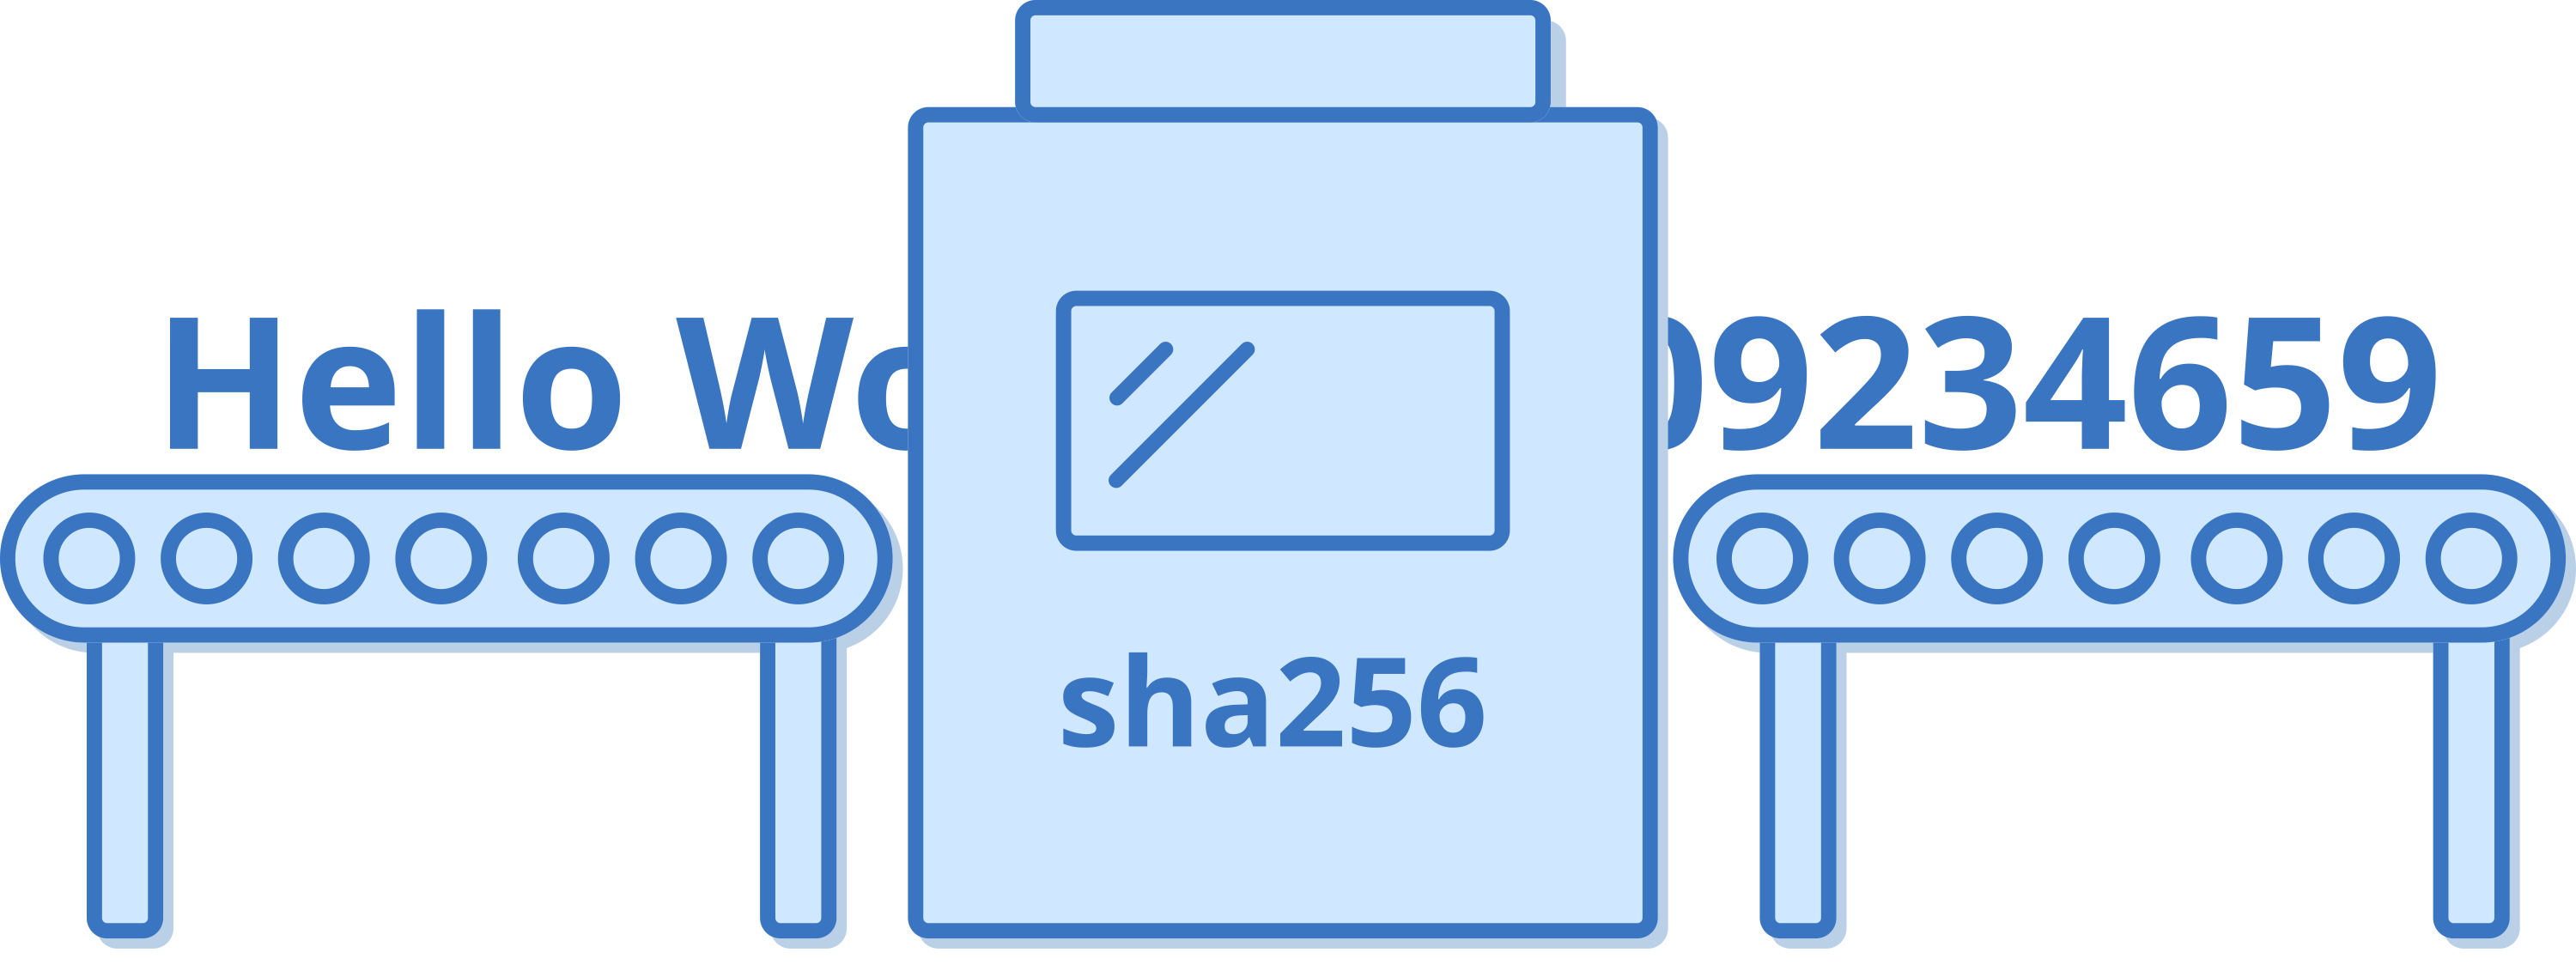
\includegraphics[width=\textwidth]{images/fig4.png}
    \caption{\footnotesize{\textit{Data gaat er aan de ene kant in, en aan de andere kant komt er een gigantisch onvoorspelbaar getal uit.}}}
    \label{fig4}
\end{figure}

De sha256 hash-functie heeft de volgende eigenschappen die nuttig zijn voor ons:

\begin{enumerate}
    \item De output is deterministisch. Dat wil zeggen dat je bij dezelfde invoer altijd dezelfde uitvoer krijgt.
    \item De uitvoer is onvoorspelbaar. Indien slechts één letter van de invoer veranderd wordt, dan is de output \textit{volledig} anders, zonder enige correlatie met de oude invoer.
    \item De uitvoer-hash is snel te berekenen, onafhankelijk van de grootte van de invoer.
    \item Het is praktisch onmogelijk twee verschillende invoerwaardes te vinden die dezelfde uitvoer hebben.
    \item De sha256 functie is een éénrichtingsfunctie. Het is onmogelijk om de invoer te herleiden uit de uitvoer.
    \item De uitvoer is altijd een specifieke grootte (256 \textit{bits} voor sha256).
\end{enumerate}

\section{Een korte uitleg over bits}

Het getallensysteem waar je bekend mee bent, bestaande uit de getallen 0 tot en met 9 wordt \textit{decimaal} genoemd omdat het tien cijfers heeft. Computers geven de voorkeur aan een ander getallenstelsel: een systeem gemaakt van enen en nullen, die respectievelijk de aan- of afwezigheid van een elektrisch signaal aangeven. Dit getallensysteem wordt \textit{binair} genoemd.

In het decimale stelsel gebruik je slechts de cijfers $0$ tot en met $9$. Als je slechts één cijfer gebruikt, kun je tien verschillende getallen vertegenwoordigen, 0 tot en met 9. Als je twee cijfers gebruikt, kun je $10 \times 10 = 100$ verschillende getallen voorstellen: $00, 01,...$ tot en met $99$. Voor drie cijfers kun je $10 \times 10 \times 10 = 1000$ getallen hebben: $000, 001,...$ tot en met $999$.

Hopelijk begin je hier een patroon in te zien. Om erachter te komen hoe groot het getal is dat we kunnen voorstellen met N cijfers, vermenigvuldigen we tien, $N$ keer met zichzelf, oftewel $10^N$ ($10$ tot de macht van $N$).

Het binaire stelsel werkt op dezelfde manier. Het enige dat verandert is het aantal cijfers die beschikbaar zijn. Terwijl we gewend zijn aan het decimaal stelsel met tien cijfers, kan een \textit{binair cijfer} of \textit{bit} slechts twee waarden hebben: nul en één.

Als een \textit{bit} 2 waarden kan vertegenwoordigen, dan kunnen twee \textit{bits} 4 waarden vertegenwoordigen: $00, 01, 10, 11$. Je kunt dit berekenen door $2 \times 2$ te vermenigvuldigen, aangezien elk cijfer twee waarden kan hebben. Drie bits kunnen $2 \times 2 \times 2 = 2^3 = 8$ waarden vertegenwoordigen:  $000, 001, 010, 011, 100, 101, 110, 111$.

Een \textit{binair} getal dat N \textit{bits} lang is, kan dus $2^N$ verschillende waarden vertegenwoordigen.

Daarom is het aantal unieke waarden die je kunt vertegenwoordigen met 256 bits, de grootte van de sha256 hashing functie, $2^{256}$. Dat is een gigantisch, bijna onvoorstelbaar groot aantal. Weergegeven in decimaal, is getal dit 78 cijfers lang. Ter vergelijking is dit ongeveer dezelfde ordegrootte als het geschatte aantal atomen in het bekende universum.

  \vspace{\baselineskip}
$2^{256}$ = 115 792 089 237 316 195 423 570 985 008 687 907 853 269 984 665 640 564 039 457 584 007 913 129 639 936
\vspace{\baselineskip} 


Bovenstaande getal is het aantal mogelijke resultaten van een sha256 hash-functie. Het is dus zo goed als onmogelijk om te voorspellen wat het getal zal zijn dat door deze functie wordt geproduceerd. Het zou hetzelfde zijn als het perfect voorspellen van de uitkomst van 256 achtereenvolgende muntworpen, of het raden van de locatie van één willekeurig uitgekozen atoom, ergens in het universum.

Dit getal is uiteraard te lang om te blijven uitschrijven, dus we houden het vanaf nu gewoon op $2^{256}$, maar ik hoop dat dit het ongelofelijke aantal mogelijkheden duidelijk heeft gemaakt.


\section{Laten we een aantal teksten hashen}

Hier zijn enkele voorbeeldteksten en hun sha256 hashes. De uitvoer wordt weergegeven in decimale notatie, maar binnenin een computer zou dit de bekende reeks van enen en nullen zijn.

Het punt is om te tonen hoe drastisch de uitvoer verandert op basis van één kleine wijziging in de invoer, en om te laten zien dat je niet kunt voorspellen welke uitvoer geproduceerd wordt door de hash-functie op basis van wat je erin stopt:

\begin{verbatim}
    “Hello World!”
    869913660443924676617831651669733090238
    07181648024718778313526389892860994842
   
    “Hello World!!”
    849402277206958989554476271088404243643
    90283616735576803008868844073193772558
    \end{verbatim}

Op geen enkele manier kan iemand op basis van deze getallen zien of berekenen wat de invoer is geweest, zelfs geen computer. Als je zelf met sha256 wilt spelen, kun je het uitproberen op \href{https://passwordsgenerator.net/sha256-hash-generator}{https://passwordsgenerator.net/sha256-hash-generator}.

\section{Hashen om de proof-of-work loterij te winnen}

Nu zijn we klaar om te praten over het belangrijkste stukje magie. We zeiden dat er $2^{256}$ totale mogelijke sha256-uitvoerwaarden zijn. Laten we in dit voorbeeld voor het gemak even doen alsof er slechts 1000 verschillende uitkomsten zijn.

Het loterijsysteem werkt als volgt:

\begin{enumerate}
    \item Alice kondigt aan dat ze 2 dollar naar \mbox{Bob} wil sturen.
    \item Iedereen die meespeelt, neemt de transactie \textquotedbl{}Alice geeft \$2 aan Bob\textquotedbl{}, en voegt hier een willekeurig getal aan toe, wat we een \textit{nonce} noemen.\footnote{Staat voor \textquotedbl{}number used only once\textquotedbl{}} Hierdoor zal de input van hun sha256 hash-functie anders zijn dan de input van die van anderen, wat helpt om een winnend getal te vinden.
    \item Als dat getal kleiner is dan het \textit{doelnummer} (dit bespreken we verder in het volgende hoofdstuk), winnen ze de loterij.
    \item Als het getal dat ze krijgen groter is dan het doelnummer, dan hashen ze opnieuw, maar voegen dit keer een andere nonce toe: \textit{\textquotedbl{}Alice geeft \$2 aan Bob nonce=12345\textquotedbl{}}, dan \textit{\textquotedbl{}Alice geeft \$2 aan Bob nonce=92435\textquotedbl{}}, dan \textit{\textquotedbl{}Alice geeft \$2 aan Bob nonce=132849012348092134\textquotedbl{}}, enzovoort. Ze doen dit net zolang tot iemand een hash heeft gevonden die kleiner is dan het doelnummer.
 \end{enumerate}   
 
Het kan vele, vele pogingen kosten om een hash te vinden die kleiner is dan het doelnummer. We kunnen in feite bepalen hoe vaak iemand de loterij kan winnen door de kans dat ze een winnend getal vinden te manipuleren. Als er 1000 mogelijke hashes zijn, en we stellen het doelnummer in op 100, welk percentage van hashes zit er dan onder de doelnummer?

Dat is natuurlijk vrij basale wiskunde; 100 van de 1000 mogelijkheden, of 100/1000 = 10\% van de hashes zullen minder zijn dan het doelnummer. Dus als je een stuk tekst hasht en je hash-functie heeft 1000 verschillende uitkomsten, verwacht je dat 10\% van de hashes onder het doelnummer van 100 uitkomt.

En dit is dus precies hoe onze loterij werkt: we spreken een doelnummer af, dan nemen we alle transacties die mensen toe willen voegen aan het grootboek, en hashen ze met een willekeurig getal erbij (de \textit{nonce}). Zodra iemand een hash vindt die onder het doelnummer valt, deelt hij dit mee aan het hele netwerk:

\vspace{\baselineskip}

Hoi iedereen!

\begin{itemize}
    \item Ik heb de transacties \textquotedbl{}Alice stuurt \$2 naar Bob\textquotedbl{} en \textquotedbl{}Charlotte stuurt \$5 naar Alice\textquotedbl{} genomen.
    \item Ik heb hier de nonce \textquotedbl{}32895\textquotedbl{} aan toegevoegd. 
    \item De hash hiervan kwam uit op 42, wat minder is dan het afgesproken doelnummer van 100.
    \item Hier is mijn proof-of-work: de transactiegegevens, de nonce die ik heb gebruikt, en de hash die werd geproduceerd op basis van die inputs.
\end{itemize}

Het heeft mij misschien miljarden hash-pogingen en duizenden dollars aan energie gekost om deze hash te vinden, maar iedereen kan onmiddellijk valideren dat ik dit werk daadwerkelijk heb gedaan; omdat ik zowel de invoergegevens (transacties en nonce) als de verwachte uitvoer (het hash-nummer) aan iedereen heb laten zien, kunnen ze dezelfde hash uitvoeren om in één poging te valideren of ik ze de juiste gegevens heb gegeven.

Hoe verhoudt dit zich tot het verbruiken van energie? We zeiden al eerder dat de set van alle mogelijke hashes eigenlijk een gigantisch getal is, dat ongeveer net zo groot is als het aantal atomen in het universum. We kunnen het doel instellen op een laag genoeg getal zodat slechts een heel klein deel van de hashes geldig is. Dit betekent dat iedereen die een geldige hash wil vinden, een enorme hoeveelheid rekentijd, en dus elektriciteit, zal moeten verbruiken om een hash te vinden die kleiner is dan ons doelnummer.

Hoe lager het doelnummer, hoe meer pogingen het kost om een geldig getal te vinden, en hoe hoger het doelnummer, hoe sneller we een winnende hash kunnen vinden. Als onze kans om het juiste getal te vinden één op een miljoen is, dan bewijzen we door dit getal te vinden dat we ongeveer een miljoen berekeningen hebben uitgevoerd.

\begin{figure}
    \centering
    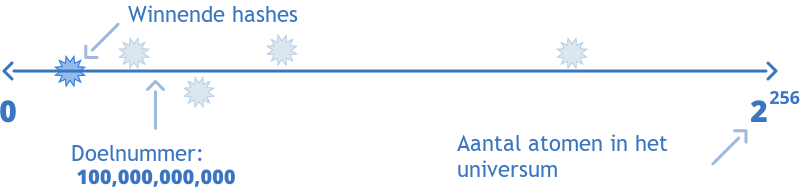
\includegraphics[width=\textwidth]{images/fig5.png}
    \caption{\footnotesize{\textit{We kunnen hashing zien als het rollen van een gigantische dobbelsteen op basis van specifieke invoergegevens, met een aantal zijden gelijk aan het aantal atomen in het universum. Alleen die invoergegevens die ervoor zorgen dat je onder het doelnummer rolt, winnen de loterij. Om de loterij te winnen, moet je aan de rest van het netwerk laten zien welke gegevens je hebt gebruikt om tot de uitkomst te komen.}}}
    \label{fig5}
\end{figure}

\chapter{Mining}

Meedoen aan de proof-of-work loterij om de mogelijkheid tot het aanpassen van het bitcoin-grootboek te winnen, is beter bekend als \textit{minen}. Dit is hoe het werkt:

\begin{enumerate}
    \item Iedereen die wil deelnemen, sluit zich aan bij het bitcoinnetwerk door hun computer aan te zetten, de juiste bitcoin-software te draaien en te luisteren naar anderen die hun transacties aankondigen.
    \item Alice kondigt haar voornemen aan om wat munten naar Bob te sturen. De computers op het netwerk \textquotedbl{}roddelen\textquotedbl{} met elkaar om deze transactie naar iedereen op het netwerk te verspreiden.
    \item Alle computers die willen deelnemen aan de loterij starten met het \textit{hashen} van de transacties waar ze over hebben gehoord door willekeurige \textit{nonces} toe te voegen aan de transactielijst en de sha256 \textit{hash}-functie uit te voeren.
    \item Gemiddeld elke tien minuten vindt een computer een hash afgeleid van de transacties die lager is dan het huidige doelnummer en wint daarmee de loterij.
    \item Deze computer maakt zijn winnende getal bekend, evenals de invoer (transacties en nonce) die ze hebben gebruikt om het winnende lot te produceren. Het kan uren gekost hebben om dat te vinden, of een paar minuten. Deze informatie bij elkaar (transacties, nonce en de hash van het proof-of-work) wordt een \textit{blok} genoemd.
    \item Alle andere deelnemers valideren het blok door te controleren of de transacties in het blok samen met de nonce inderdaad hashen tot wat er gedeeld wordt, dat de hash inderdaad lager is dan het doelnummer, dat het blok geen ongeldige transacties bevat én dat de geschiedenis in het blok niet in strijd is met voorgaande blokken.
    \item Iedereen schrijft het blok in zijn kopie van het grootboek en voegt het toe aan de bestaande ketting van blokken, bekend als een \textit{blockchain}.
\end{enumerate}

Dat is het in een notendop. We hebben ons eerste blok geproduceerd en mogen onze eerste transacties aan onze grootboeken toevoegen.

Misschien heb je in de media de vaak herhaalde bewering gelezen dat bitcoin mining het oplossen van ingewikkelde vergelijkingen inhoudt. Nu zul je begrijpen dat dit volstrekt onjuist is; in plaats van vergelijkingen op te lossen, moet je bij bitcoin mining herhaaldelijk gooien met een grote virtuele dobbelsteen om een hash te produceren die onder een bepaald doelnummer valt. Het is gewoon een kansspel dat deelnemers dwingt om een bepaalde hoeveelheid elektriciteit te verbruiken.

\section{Hoe worden nieuwe bitcoins gemaakt?}

Tot nu toe hebben we besproken hoe Alice \$2 naar Bob kan sturen. We gaan vanaf nu stoppen met praten over dollars, want bitcoin kent geen dollars. Wat we wel hebben, zijn bitcoins zelf: digitale eenheden die waarde vertegenwoordigen op het bitcoinnetwerk.

Om bij ons voorbeeld te blijven, kunnen we zeggen dat Alice 2 bitcoins naar Bob stuurt door aan te kondigen dat ze haar munten, die op haar \textquotedbl{}rekening\textquotedbl{} staan, naar die van Bob overzet. Vervolgens wint iemand de proof-of-work loterij, en wordt haar aangekondigde transactie toegevoegd aan het grootboek.

Maar waar kwamen die 2 bitcoins van Alice oorspronkelijk vandaan? Hoe ging bitcoin van start en hoe verwierf iemand ooit munten voordat er marktplaatsen waren om ze te kopen met traditionele fiatvaluta zoals dollars of euro’s?

Toen Satoshi bitcoin ontwierp, had hij ervoor kunnen kiezen om een database te maken die alle 21 miljoen munten aan hem toewees en vervolgens iedereen te vragen ze van hem te kopen. Echter zou er weinig reden zijn voor anderen om waarde toe te kennen aan een systeem waarin één enkeling alle waarde bezat. Hij kon een register gemaakt hebben waar mensen konden intekenen met een e-mailadres om kans te maken op enkele munten. Maar een registratiesysteem zou vatbaar zijn aan een zogenaamde \textit{Sybil-aanval}, aangezien het quasi gratis is om miljoenen e-mailadressen aan te maken.\footnote{Een Sybil-aanval is een aanval waarin een deelnemer aan een bepaald netwerk een groot aantal pseudonieme addressen aanmaakt om een grote hoeveelheid invloed in het netwerk te vergaren; vernoemd naar Sybil, een boek over een vrouw met een dissociatieve identiteitsstoornis}

Satoshi koos uiteindelijk om de nieuwe munten te laten genereren door het proces van minen, oftewel de deelname aan de proof-of-work loterij om het recht te verkrijgen in het grootboek te schrijven. Wanneer je een grote hoeveelheid energie gebruikt en het winnende getal van het volgende geldige blok vindt, krijg je het recht om de transacties die bij jou bekend zijn toe te voegen aan het grootboek. Daarbovenop mag je ook een speciale transactie toevoegen aan het blok die we een \textit{coinbase}-transactie noemen. Zo’n transactie zegt: \textquotedbl{}12,5 bitcoin werden gemaakt en toegekend aan Marie de Miner om haar te compenseren voor de energie die gebruikt werd om het blok te vinden.\textquotedbl{}

Dit is hoe nieuwe bitcoins \textquotedbl{}gemaakt\textquotedbl{} worden. Met dit proces is iedereen ter wereld in staat om hun eigen munten te vergaren zonder tussenkomst van een centrale autoriteit én zonder hun identiteit bekend te moeten maken. De enige vereiste is dat ze genoeg willen betalen voor de elektriciteit die nodig is om mee te doen met de loterij. Dit maakt bitcoin’s uitgifte resistent tegen \textit{sybil}-aanvallen. Wie munten wil, zal energie moeten verbruiken en iets moeten betalen om ze te maken.

\section{De blokbeloning}
De persoon die de loterij wint, mag zichzelf enkele vers gemaakte munten toekennen. Maar waarom is de beloning 12,5 bitcoins en niet 1000? Waarom kan niemand valsspelen en zichzelf een willekeurig bedrag toekennen?

Bitcoin is een systeem van gedistribueerde consensus. Dit betekent dat iedereen akkoord moet gaan met wat geldig is en wat niet. Dat kan door software op je computer te draaien die een bekende set van regels afdwingt. Deze regels staan bekend als de consensusregels van bitcoin. Wanneer een miner een nieuw blok vindt, wordt alles tegen de consensusregels afgewogen. Wanneer het blok geldig blijkt te zijn, schrijft iedereen het in hun grootboek en wordt het geaccepteerd als waarheid. Indien niet, dan wordt het blok verworpen.

Hoewel de volledige lijst van consensusregels vrij complex is, kunnen we de belangrijkste hieronder opsommen:

\begin{itemize}
    \item Een geldig blok mag een specifieke hoeveelheid nieuwe munten aan het netwerk toevoegen, zolang het voldoet aan de regels van het uitgifteschema wat vastgelegd is in de software.
    \item Transacties moeten geldige handtekeningen hebben die aangeven dat de eigenaar het verzenden daadwerkelijk goedgekeurd heeft.
    \item Transacties die munten proberen uitgeven die al eerder uitgegeven werden, kunnen onder geen geval plaatsvinden.
    \item De hoeveelheid data in het blok mag een specifieke limiet niet overschrijden.
    \item De proof-of-work hash van het blok moet kleiner zijn dan het huidige doelnummer, waardoor onbetwistbaar aangetoond wordt dat dit blok tot stand kwam door een bepaalde hoeveelheid elektriciteit te gebruiken.
\end{itemize}

Indien Marie een blok vindt en beslist om zichzelf een beetje extra te geven, dan zullen de computers van de overige deelnemers dit blok afwijzen en als ongeldig beschouwen. Dit komt omdat de bitcoin-software die iedereen draait een stukje code bevat dat zegt: “de huidige blokbeloning is precies 12,5 bitcoins. Als je een blok ziet waarin iemand meer dat dit bedrag toekent, verwerp het dan.”

Als Marie probeert vals te spelen en een ongeldig blok produceert, dan komt het blok in niemands grootboek terecht en zal ze simpelweg veel elektriciteit verspild hebben om een vervalsing te produceren die niemand wil. Dit geeft bitcoin een \textit{onvervalsbare kostbaarheid}, een term die werd geïntroduceerd door Nick Szabo in zijn esssay \textquotedbl{}Shelling Out\textquotedbl{}. Het is vrij makkelijk te begrijpen dat geld wat makkelijk te vervalsen is, nooit daadwerkelijk nuttig kan zijn als geld. Het is onmogelijk om bitcoin te vervalsen omdat iedere munt op echtheid te controleren valt met een simpele, wiskundige test.

Satoshi ontgon het eerste \textquotedbl{}genesis\textquotedbl{} blok, wat de eerste bitcoins ooit produceerde. De code is \textit{open source} en dus kan iedereen een kijkje onder de motorkap nemen om te zien of er niets verkeerd loopt. Maar zelfs Satoshi moest miljarden berekeningen doen en meespelen met de proof-of-work loterij om die eerste blokken te vinden. Op geen enkele manier kon hij een vervalsing produceren door te liegen over de energie die hij nodig had om een winnende oplossing te vinden. En dat terwijl hij de ontwerper van het systeem was.

Iedereen die zich daarna bij het netwerk aansloot kon controleren dat zijn gevonden oplossingen voldeden aan de vereisten. Door ze naast het initiële doelnummer en transactiedata te leggen, blijkt overduidelijk dat een bepaalde hoeveelheid energie gebruikt werd om een statistisch zeldzaam doelnummer te vinden. Stel je voor dat het mogelijk is om met diezelfde precisie en regelmaat te controleren hoe fiatvaluta in het traditionele bankensysteem tot stand komt.

\section{De halvering}
Het proces van minen produceert nieuwe bitcoins. Maar Satoshi wou een systeem waarin het onmogelijk was om de waarde van de munt te devalueren. Hij wou niet dat het monetaire aanbod tot in het oneindige zou blijven stijgen. In plaats daarvan, ontwierp hij een uitgifteschema dat snel begon en geleidelijk afneemt tot uiteindelijk geen nieuwe munten meer zullen worden geproduceerd.

In het begin was de beloning voor een blok 50 bitcoin en dat is hoeveel Satoshi ontving voor zijn allereerste ontgonnen blok. Net zozeer kregen alle andere deelnemers die zich aansloten bij het netwerk in de begindagen voor elke gevonden blok 50 bitcoin.

De bitcoin-software dwingt iedere vier jaar een halvering van de blokbeloning af. De periode is gebaseerd op het aantal blokken in plaats van een bepaalde periode van tijd, maar omdat blokken ongeveer elke tien minuten worden geproduceerd, maakt dit in werkelijkheid weinig verschil. In 2008 was de blokbeloning 50 BTC, in 2012 was het 25 BTC, in 2016 12,5. Vandaag, op 8 juni 2019, zijn al 579.856 blokken ontgonnen sinds het begin van bitcoin en is de beloning 12,5 BTC per blok.

Binnen 50.144 blokken, ongeveer in mei 2020, zal de beloning verlaagd worden tot 6,25 BTC per blok. De jaarlijkse toename van het aanbod wordt dan ongeveer 1,8\%. Na nog eens 12 jaar, 3 halveringen later, zullen 99\% van alle bitcoins in circulatie zijn en krijgen miners nog minder dan 1 bitcoin per gevonden blok. Je kan de voortgang van de halveringen volgen op \href{https://bitcoinblockhalf.com}{https://bitcoinblockhalf.com}.

\begin{figure}
    \centering
    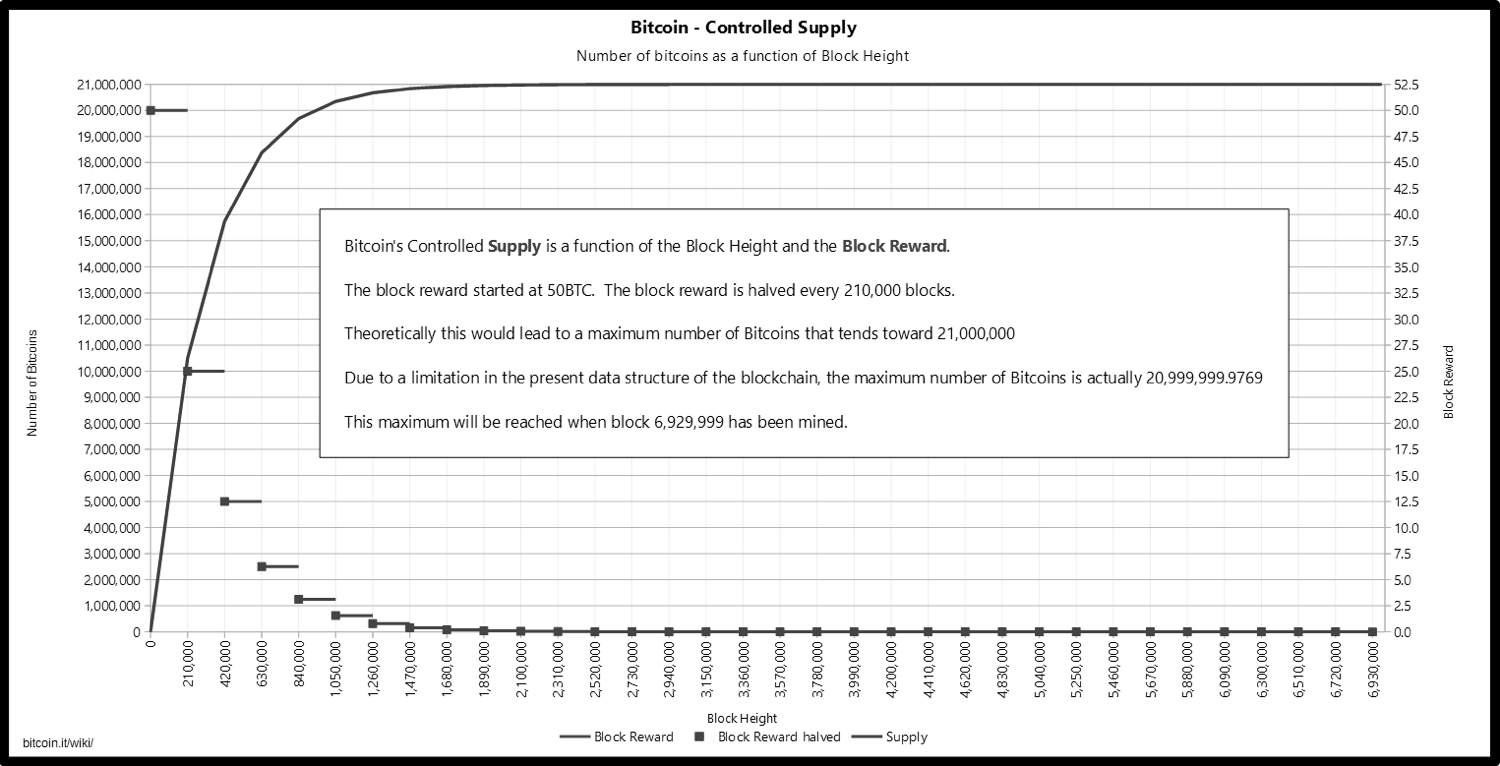
\includegraphics[width=\textwidth]{images/fig6.png}
    \caption{\footnotesize{\textit{Het gecontroleerde monetaire tijdschema van bitcoin kan door iedereen worden bevestigd.}}}
    \label{fig6}
\end{figure}

Uiteindelijk, rond het jaar 2140, zal de blokbeloning volledig wegvallen en moeten miners genoegen nemen met transactievergoedingen van de gebruikers als compensatie voor hun werk.

De blokbeloningen, en het uitgifteschema in het algemeen, worden afgedwongen in de bitcoin-software die, zoals eerder gesteld, volledig \textit{open source} is en dus door iedereen volledig gevalideerd kan worden. Een blok produceren dat niet voldoet aan de regels zal door niemand met dezelfde software geaccepteerd worden.

\section{Beheersen van de uitgifte en het blokinterval}

Het minen van bitcoin vereist computers en elektriciteit. Dus hoe meer computers en elektriciteit je ter beschikking hebt, hoe groter de kans is dat jij een winnend lot weet te vinden. Stel, het netwerk bestaat uit 100 computers met gelijke rekenkracht en jij bezit daar 10 van. Dit betekent dat je in ongeveer 10\% van de gevallen een winnende oplossing zal vinden. Maar mining is een proces waar geluk en willekeur mee gemoeid gaat. Het is dus theoretisch gezien mogelijk dat er uren of dagen voorbijgaan zonder dat je een winnend lot vind.

In het vorige deel hebben we uitgelegd dat miners zichzelf niet simpelweg een arbitraire blokbeloning kunnen toekennen. Die zouden door andere \textit{nodes} verworpen worden. Maar wat als ze een heleboel energie gebruikten om het miningproces sneller te laten verlopen en zo meer bitcoins te verwerven? Dit zou in strijd zijn met het opzet in het ontwerp van bitcoin, namelijk dat het uitgifteschema van tevoren bekend zou moeten zijn.

Laten we opnieuw het eerder gegeven voorbeeld nemen: er zijn 1000 mogelijke hashes en ons doelnummer is 100. In 10\% van de gevallen zullen we een getal vinden dat kleiner is dan 100 en een geldig blok vinden.

Stel dat het 1 seconde duurt om elke hash te berekenen. Als we iedere seconde “onze dobbelsteen rollen” door de huidige transacties en onze lukrake \textit{nonce} te hashen, vinden we in 10\% van de keren een getal dat kleiner is dan het doelnummer. We verwachten dus dat het ons gemiddeld 10 seconden vergt om een geldige hash te vinden.

Wat gebeurt er wanneer 2 computers meedoen aan de loterij? Ze hashen dan dubbel zo snel en verwachten een geldige hash iedere 5 seconden. Wat als 10 computers meedoen? Elk van hen kan ongeveer iedere seconde een winnende oplossing vinden.

Het probleem is dus het volgende: als meer mensen meedoen, worden blokken te snel geproduceerd. Dit leidt tot twee uitkomsten die we niet willen:

\begin{enumerate}
    \item Het is niet meer mogelijk om een vooraf vastgesteld uitgiftescheme aan te houden. We willen hiervoor ieder uur een relatief consistent aantal bitcoins in circulatie zien komen om te zorgen dat het proces tot in het jaar 2140 duurt, en niet eerder ten einde komt.
    \item Het creëert problemen op het netwerk: wanneer blokken te snel gevonden worden en geen tijd hebben om de rest van het netwerk te bereiken voordat een volgend blok gevonden wordt, kunnen we niet tot consensus komen over de lineaire geschiedenis van transacties. Verschillende miners zouden dan transacties in hun blokken gestopt kunnen hebben, die al uitgegeven werden in een vorig blok waar ze nog niet van op de hoogte waren.
\end{enumerate}

Als minder mensen minen dan hebben we het tegenovergestelde:

\begin{enumerate}
    \item Nieuwe bitcoins worden te traag uitgegeven waardoor het uitgifteschema niet klopt.
    \item Het systeem wordt onbruikbaar omdat je soms uren, dagen of langer zal moeten wachten om je transacties in het grootboek te krijgen.
\end{enumerate}

Het totale aantal hashes per seconde van alle miners op het netwerk noemen we de \textit{hash-rate}.



\begin{figure}
    \centering
    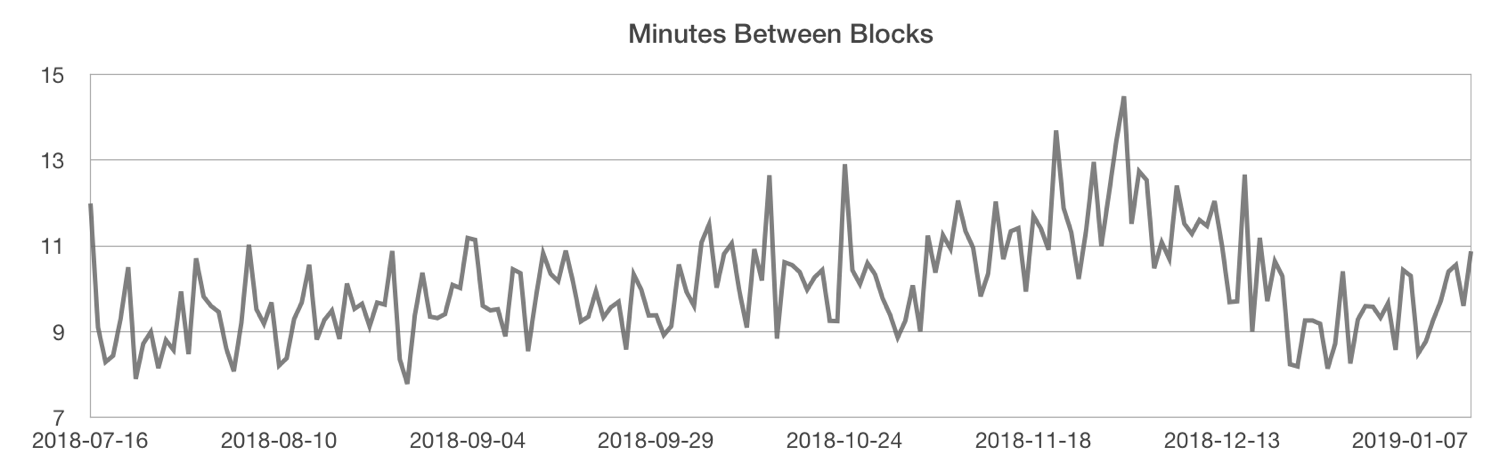
\includegraphics[width=\textwidth]{images/fig7.png}
    \caption{\footnotesize{\textit{De tijd tussen blokken varieert afhankelijk van de hash-rate die komt en gaat, evenals willekeurige kans.}}}
    \label{fig7}
\end{figure}


\section{Moeilijkheidsaanpassing: consensus over het doelnummer}

Aangezien bitcoin een vrijwillig en permissieloos systeem is waar mensen deel aan kunnen nemen zoals zij willen, zonder dat iemand de leiding heeft, zal het aantal miners op het netwerk sterk schommelen. We hebben een manier nodig om de productie van blokken stabiel te houden in plaats van telkens een versnelling of vertraging in productie te zien wanneer miners zich aansluiten of verdwijnen.

Hoe kunnen we het moeilijker maken om geldige hashes te vinden als meer spelers meedoen aan de loterij en makkelijker wanneer spelers weggaan? Op die manier zouden we de uitgifte en blokintervallen stabiel kunnen houden.

Herinner je dat het minen van bitcoin een loterij is waarin je een willekeurig getal moet vinden dat kleiner is dan het doelnummer.


\begin{figure}
    \centering
    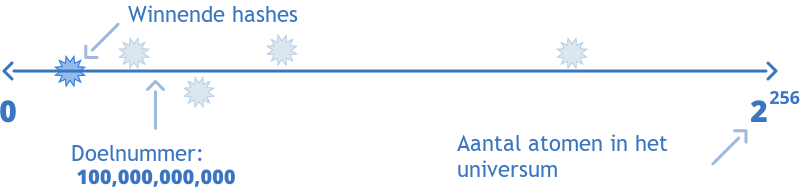
\includegraphics[width=\textwidth]{images/fig5.png}
    \caption{\footnotesize{\textit{We proberen deze kleine ruimte te raken. Het aantal mogelijke uitkomsten is extreem groot, dus het zal heel lang duren om daar te komen door willekeurige worpen van de dobbelsteen.}}}
    \label{fig8}
\end{figure}


Bitcoin lost dit probleem op door middel van een \textit{aanpassing van de moeilijkheidgraads}. Omdat iedereen dezelfde code draait die dezelfde regels afdwingt, én iedereen een volledige kopie heeft van de transactiegeschiedenis, kan iedereen onafhankelijk berekenen hoe snel blokken op dat moment geproduceerd worden.

Telkens wanneer we 2016 blokken geproduceerd hebben (ongeveer 2 weken)\footnote{De aanpassingsperiode van 2016 blokken is op basis van het beoogde blokinterval van 10 minuten; 10 minuten x 2016 blokken = twee weken. Het blokinterval werd arbitrair vastgesteld door Satoshi om groot genoeg te zijn zodat de meeste nodes kunnen op de hoogte zijn van de laatste blok. De periode van twee weken is ook ietwat arbitrair gekozen, maar is ontworpen om te voorkomen dat het spel belazerd wordt door te snelle achtereenvolgende aanpassingen in de hash-rate.}, analyseren we de snelheid van uitgifte over de afgelopen periode. We kijken hoeveel tijd nodig was om die 2016 blokken te produceren en passen vervolgens passen het doelnummer aan om de productie van blokken te versnellen of te vertragen.

Iedereen neemt de laatste 2016 blokken en deelt ze door de tijd die gemiddeld nodig was om te ze creëren. Was het gemiddelde meer dan 10 minuten? Dan gaan we te traag. Lag het gemiddelde onder de 10 minuten? Dan gaan we te snel.

We kunnen nu het doelnummer aanpassen zodat het groter of kleiner is, proportioneel met hoe traag of snel we gaan, om te zorgen dat we in lijn blijven met het afgesproken interval van 10 minuten.

Het doelnummer kan een groter getal worden, waardoor een groter bereik van hashes een geldige oplossing wordt. Hierdoor wordt de kans om een winnende hash te vinden voor de miners groter en hoeven ze minder energie te gebruiken om een blok te vinden. Dit heet \textit{de moeilijkheidsgraad verlagen}.

\begin{figure}
    \centering
    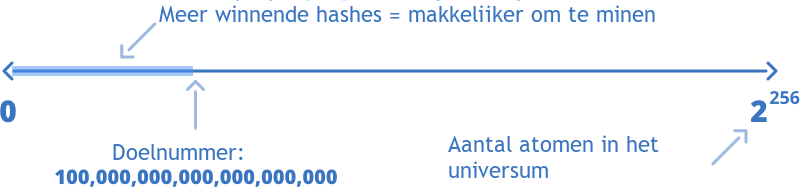
\includegraphics[width=\textwidth]{images/fig8.png}
    \caption{\footnotesize{\textit{Het verhogen van het doel vergroot de geldige ruimte, waardoor het waarschijnlijker wordt om in minder pogingen een juiste oplossing te vinden. Daardoor wordt het goedkoper in verbrande \mbox{energie.}}}}
    \label{fig9}
\end{figure}



Anderzijds, kunnen we het doelnummer kleiner maken zodat er minder hashes geldig zijn en miners meer energie moeten spenderen om een blok te vinden. Dit heet \textit{de moeilijkheidsgraad verhogen}.

Dit betekent dat we voor elke periode van 2016 blokken precies weten wat het doelnummer is. Het geeft ons de magische grens waarbinnen een hash van de proof-of-work moet vallen om een winnend lot te bemachtigen, binnen die periode.

De aanpassingen van de moeilijkheidsgraad en het doelnummer is misschien wel de belangrijkste innovatie van bitcoin. Het stelt iedereen in staat om onafhankelijk de lotnummers te verifiëren, die op hun beurt weer gebaseerd zijn op een doelnummer dat ook onafhankelijk te verifiëren is. Hierdoor kunnen we een loterij spelen zonder dat iemand ons de winnende combinatie hoeft te vertellen.



In Figuur \ref{fig10} zie je de \textit{hash-rate} (lijn) en de moeilijkheidsgraad (staven) doorheen de tijd. De moeilijkheid wordt iedere 2016 blokken aangepast en lijkt een beetje op een trap. Telkens wanneer de hash-rate boven de moeilijkheid uitstijgt, zie je dat de moeilijkheidsgraad stijgt om bij te benen. Wanneer de hash-rate zakt, zoals tussen oktober en december 2018, zakt ook de moeilijkheidsgraad. De aanpassing van de moeilijkheidsgraad volgt altijd wat de hash-rate doet met een vertraging van 2016 blokken (twee weken).

\begin{figure}
    \centering
    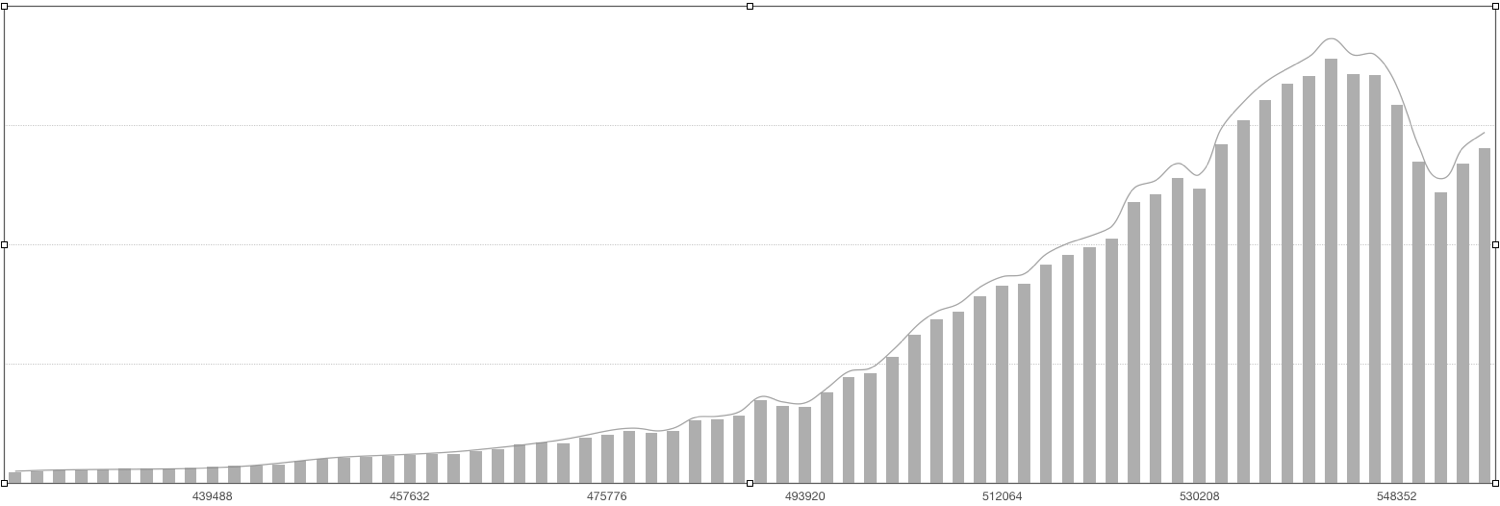
\includegraphics[width=\textwidth]{images/fig10.png}
    \caption{\footnotesize{\textit{Hash-snelheid versus moeilijkheid.}}}
    \label{fig10}
\end{figure}

Omdat er een vertraging van 2016 blokken op de aanpassing zit, is het mogelijk dat grote pieken omhoog of omlaag in hash-rate leiden tot een over- of onderproductie van bitcoins tijdens dat interval en licht afgeweken wordt van het uitgifteschema.

Het verhogen van de hash-rate gaat gepaard met de productie van een grote hoeveelheid nieuwe hardware, waardoor pieken relatief ongebruikelijk zijn en niet al te veel impact hebben. Het effect van iedere piek, omhoog of omlaag, zal beperkt blijven tot dat interval van 2016 blokken. Na de volgende aanpassing komen we opnieuw bij een gemiddelde van 10 minuten per blok.

\section{Hash-rate en de dollarwaarde van bitcoin}
Bitcoin herberekent de moeilijkheidsgraad automatisch op basis van alle rekenkracht van de loterijspelers. Dit zijn de miners die energie verbruiken om te hashen. Op die manier raakt de echte wereld vervlochten met onze digitale wereld. De prijs van bitcoin, de prijs van hardware en energie en de moeilijkheid van het doelnummer creëren feedback-koppelingen:

\begin{enumerate}
\item Speculanten kopen bitcoin omdat ze denken dat de prijs hoger gaat, waardoor ze de prijs opdrijven tot \$X.
\item Miners verbruiken tot \$X aan energie en hardware om bitcoins te verdienen.
\item Een grote vraag van kopers duwt de prijs omhoog en leidt tot meer miners die aardig verdienen aan hun activiteit.
\item Meer miners betekent meer hash-rate en meer verbruikte energie om bitcoin te produceren. Het netwerk wordt nog sterker beveiligd. De kopers worden gerustgesteld door de veiligheid van het netwerk en drijven de prijs soms nog verder omhoog.
\item Na 2016 blokken gaat de moeilijkheidsgraad omhoog door de aanwezigheid van meer hash-rate.
\item Een hogere moeilijkheid betekent een lager doelnummer. De miners vinden nu minder vaak blokken waardoor sommigen meer dan \$X spenderen in kosten om een bitcoin te minen.
\item Voor sommige miners blijkt het niet meer interessant om te minen, omdat ze meer energie verbruiken dan de winst die hun activiteit oplevert wanneer ze hun bitcoin verkopen. Ze leggen hun machines af en de hash-rate op het netwerk gaat terug omlaag.
\item De volgende 2016 blokken passeren. De moeilijkheid wordt opnieuw berekend en aangezien sommige miners offline gingen, wordt het deze keer makkelijker. Het doelnummer gaat omhoog.
\item De lagere moeilijkheid betekent dat miners, die voorheen onrendabel waren, hun machines terug aanzetten of dat nieuwe miners op het toneel verschijnen.
\item Ga terug naar 1.
\end{enumerate}
In een neerwaartse markt kan de cyclus in de andere richting gaan. Gebruikers van het netwerk dumpen dan hun munten, de prijs gaat omlaag en miners worden onrendabel.

Het algoritme voor de aanpassing van de moeilijkheidsgraad zorgt dat er altijd een evenwicht wordt gevonden tussen de prijs en de hoeveelheid hash-rate die aanwezig is op het netwerk. Zelfs als de prijs drastisch zou zakken en de helft van de huidige hash-rate uit het netwerk zou duwen, dan zou de volgende aanpassing het opnieuw rendabel maken op een nieuw evenwichtsniveau.

De aard van de moeilijkheidsaanpassing duwt inefficiënte miners eruit ten voordele van degenen die werken met de goedkoopst mogelijke energie en met de laagste totale operationele kosten. Na verloop van tijd dwingt het bitcoin miners richting afgelegen hoeken op de planeet. Ze gebruiken energiebronnen die onderbenut of volledig onontgonnen zijn. Een rapport van CoinShares uit 2019 schat dat ongeveer 75\% van de bitcoin miners hernieuwbare energie gebruikt.\footnote{Lees meer over de laatste stand van zaken betreffende mining op \href{https://coinshares.com/research/bitcoin-mining-network-june-2019 }{https://coinshares.com/research/bitcoin-mining-network-june-2019 }}

De laatste jaren ging de prijs pijlsnel omhoog, net als de totale hash-rate. Hoe hoger de hash-rate, hoe moeilijker het is om het netwerk aan te vallen. Om te bepalen wat in het grootboek komt, moet je ten minste evenveel energie en hardware beheren als de helft van het hele netwerk. Op vandaag wordt geschat dat de elektriciteit die gebruikt wordt door bitcoin miners equivalent is met het verbruik van een land van gemiddelde grootte.

\section{Vergoedingen en het einde van blokbeloning}

Hoe zorgen we dat miners nog altijd een drijfveer hebben om energie te spenderen om het netwerk te beveiligen wanneer de blokbeloning uiteindelijk afloopt? Het antwoord zijn de vergoedingen voor transacties. Met tijd vervangen de vergoedingen de beloning en ze geven de miners ook de drijfveer om transacties daadwerkelijk in een blok te plaatsen. Anders zouden ze perfect lege blokken kunnen produceren en enkel de blokbeloning opstrijken.

De vergoedingen worden bepaald op een vrije markt waar gebruikers bieden voor de schaarse ruimte binnen een blok. Gebruikers die transacties versturen geven aan hoeveel vergoeding ze willen betalen aan miners. Op hun beurt kunnen de miners de transactie al dan niet insluiten in het volgende blok, afhankelijk van de vergoedingen. Wanneer slechts weinig transacties in het volgende blok willen, zijn de vergoedingen laag en is er weinig competitie. Wanneer de ruimte in de blokken opgevuld raakt, gaan gebruikers meer bereid zijn om een hogere vergoeding te betalen om hun transactie sneller bevestigd te zien (in de volgende blok). Wie niet wil betalen kan zijn transactievergoeding laag zetten, maar moet dan rekening houden met een langere wachttijd.

In traditionele financiële systemen zijn vergoedingen doorgaans gebaseerd op een percentage van het bedrag van de transactie. In bitcoin is de waarde van de transfer niet relevant voor de vergoeding. In plaats daarvan, zijn vergoedingen proportioneel met de schaarse grondstof die ze consumeren: \textit{blokruimte}. De vergoedingen worden gemeten in satoshi’s per byte opgebruikte ruimte in een blok.\footnote{Een byte is 8 bits.} Op die manier kan het zijn dat een transactie van een miljoen bitcoin tussen twee personen goedkoper is qua vergoeding dan een transactie die 1 BTC splits in 10 ontvangers aangezien die laatste meer ruimte zal innemen in de transactielijst.

Tijdens periodes waarin bitcoin enorm in trek was, zoals de grote stierenmarkt van 2017, gingen transactievergoedingen door het dak. Sindsdien zijn een aantal nieuwe functies geïmplementeerd die het probleem van hoge transactiekosten op het netwerk verlichten.

Een van die aanpassingen is \textquotedbl{}Segregated Witness\textquotedbl{}. Deze aanpassing zorgt voor een andere voorstelling van de data in blokken. Transacties die gebruik maken van die upgrade kunnen meer dan de originele 1MB aan blokruimte gebruiken (via een aantal slimme trucs die niet verder toegelicht worden in dit boek).

Nog iets dat bijdraagt aan het verlagen van de hoge transactiekosten is \textit{batching}. Grote handelsbeurzen en -platformen in het ecosysteem begonnen met het bundelen van transacties voor verschillende gebruikers in één: in tegenstelling tot traditionele betalingen via de bank of PayPal, die altijd geld van één persoon naar een andere sturen, kan een bitcointransactie een groot aantal inputs combineren en een groot aantal outputs produceren. Een beurs die bitcoin wil versturen om uit te betalen aan 100 verschillende gebruikers kan dat dus perfect doen in een enkele transactie. Op die manier wordt schaarse blokruimte veel efficiënter gebruikt. Wat ogenschijnlijk slechts enkele transacties per seconde zijn, kunnen in realiteit perfect duizenden transacties inhouden.

Met \textit{SegWit} en \textit{batching} komen we al een heel eind om de vraag naar blokruimte te verlagen. Verdere verbeteringen zullen het gebruik van blokruimte nog efficiënter maken. Niettemin zal er opnieuw een dag komen dat transactievergoedingen terug oplopen en blokken door de grote vraag naar blokruimte weer voller en voller raken.

We hebben nu bijna alle aspecten van bitcoin onder de loep genomen:

\begin{enumerate}
\item Centrale bank vervangen door een gedistribueerd grootboek.
\item Een loterij opgezet om te bepalen wie in het grootboek mag schrijven.
\item Spelers van de loterij worden verplicht om energie te gebruiken om lotjes te bemachtigen (door te hashen). Het is voor iedereen eenvoudig om een winnend lot te verifiëren door de hash naast ons eigen, onafhankelijk bepaald, doelnummer te leggen.
\item Duidelijke regels voor de deelnemers: wie de regels niet volgt, zal niet geaccepteerd worden. Hun blok met beloning in de zogenaamde \textit{coinbase}-transactie wordt dan verworpen en ze ontvangen geen bitcoin. Op die manier ontmoedigen we valsspelen en bieden we een economische stimulans om de regels te volgen.
\item Controle over de timing en selectie van het doelnummer voor de loterij door iedereen te laten berekenen wat het doelnummer moet zijn op basis van vastgelegde regels in de software en de geschiedenis van de laatste 2016 blokken.
\item Handhaven van het uitgifteschema door moeilijkheidsgraad aan te passen als gevolg van een hogere of lagere hash-rate.
\item Gebruik van \textit{open source} code om ervoor te zorgen dat iedereen voor zichzelf kan verifiëren dat zij dezelfde regels hanteerden betreffende geldigheid van transacties, blokbeloning en moeilijkheidsaanpassing.
\end{enumerate}
Geen centrale autoriteit meer. We hebben nu een volledig gedistribueerd en decentraal systeem. Dat is bijna het volledige plaatje. Eén probleem rest ons nog. Wanneer een nieuwe deelnemer aansluit bij het netwerk en een kopie van het grootboek opvraagt, kunnen ze van verschillende \textit{nodes} afwijkende geschiedenissen ontvangen. Hoe zorgen we voor een enkele, lineaire geschiedenis en hoe voorkomen we dat miners het verleden herschrijven?







\chapter{Het grootboek beveiligen}
We hebben besproken hoe we erin slagen om kopieën bij te houden van, en te schrijven naar een gedistribueerd grootboek dat zonder dwang of corruptie werkt. We doen dit met behulp van een loterij en op basis van validatie door consensus.

Maar wat gebeurt er wanneer een loterijwinnaar besluit om zich kwaadwillig op te stellen? Kan een miner historische boekingen in het grootboek aanpassen? Kunnen onze kwaadwillige actoren Eva, Davy en Femke samenspannen en de geschiedenis herschrijven of rekeningsaldi wijzigen en zichzelf meer munten toekennen?

In dit deel gaan we de \textit{blockchain} bespreken. Eigenlijk is het louter een marketingterm die de technologiesector binnengedrongen is. In bitcoin worden blokken aan elkaar gehecht om een duidelijk link van de ene transactie naar de volgende te behouden. Een ketting van blokken, een \textit{blockchain}, dus. Hierdoor ontstaat een lineaire geschiedenis van creatie en uitgaven sinds Satoshi’s \textit{genesis block }in 2009 tot op vandaag.

In het vorige deel hebben we een klein beetje gelogen om het eenvoudig te houden. Wanneer je meespeelt met de loterij (om te minen), is het niet enkel de wachtende transacties en een lukrake \textit{nonce} die je hasht. Je voegt daar ook nog een hash van het blok net daarvoer toe. Op die manier ontstaat een duidelijke link tussen jouw blok en het vorige.

Herinner je dat de output van een hash-functie onvoorspelbaar is en afhankelijk is van alle inputdata die je gebruikt. De hashes van ons blok bevat nu drie verschillende inputs:

\begin{enumerate}
    \item De transacties die we naar het grootboek willen schrijven
    \item Een lukrake \textit{nonce}
    \item Een hash van de vorige blok die we gebruiken als basis voor de geschiedenis van ons grootboek.
\end{enumerate}




\begin{figure}
    \centering
    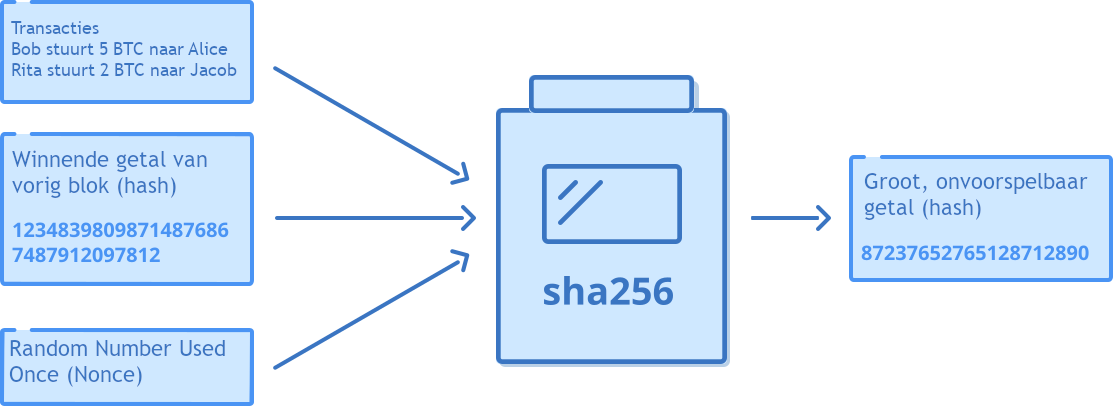
\includegraphics[width=\textwidth]{images/fig11.png}
    \caption{\footnotesize{\textit{De drie inputs die zijn gebruikt om een hash voor de loterij te bouwen, bevatten nu ook de vorige winnende hash, waardoor een link ontstaat van het ene blok naar het andere.}}}
    \label{fig11}
\end{figure}


Dit stelt ons in staat om een historisch overzicht van elk blok te bouwen tot en met het eerste blok, ontgonnen door Satoshi. Wanneer we een nieuw blok aan de ketting toevoegen, moeten we valideren dat het geen transacties bevat die bitcoins uitgeven die in het verleden al een gespendeerd zijn.

Wanneer ook maar iets verandert in de inputs van de hash, zal de output van de hash drastisch en onvoorspelbaar anders zijn. Als je probeert de data uit een oud blok te manipuleren, zal je ook de resulterende hash veranderen. Aangezien die hash ook werd gebruikt in de input voor de blokken die daar net na kwamen, zal je ook de hashes van die blokken veranderen. De hash van de laatste blok in de ketting, die gelinkt is met alle voorgaande, doet dienst als een vingerafdruk voor de volledige geschiedenis van het grootboek tot op dat moment.

Het is onmogelijk om vals te spelen bij proof-of-work omdat iederen weet hoeveel energie gebruikt moet worden per blok om het vereiste doelnummer te vinden. Mocht iemand willen proberen om een oudere blok in de ketting aan te passen, zouden ze de proof-of-work hash moeten aanpassen van de blok waar ze mee knoeien én die van alle andere blokken die daarna komen. De \textit{blockchain} is niet alleen fraudebestendig, het is ook enorm duur om het te proberen.

Iedere nieuwe blok die gevonden wordt draagt effectief bij aan de veiligheid van alle blokken die ervoor kwamen omdat het de hoeveelheid elektriciteit die nodig is om de proof-of-work hashes voor de ketting tot op dat punt te herschrijven, verhoogt. Een transactie in een blok, begraven onder 6 opeenvolgende blokken wordt aanzien als finaal door de meeste handelaars. Het zou namelijk een aanzienlijke hoeveelheid energie kosten om de laatste 6 blokken opnieuw te hashen met de hash-rate van vandaag. Een transactie die 100 blokken diep zit? Vergeet het maar.

Wanneer je een kopie van de \textit{blockchain} downloadt, is elke transactie in elke blok volledig transparant. Je kan de proof-of-work hashes zelf controleren om zeker te zijn dat niets aangepast werd door de persoon die jouw het grootboek bezorgde.

\section{Wanneer blokken botsen}
Er ontbreekt nog een element in het consensus-systeem: hoe zorgen we dat iedereen met dezelfde lineaire geschiedenis van transacties werkt wanneer miners tegelijk twee blokken vinden en ze naar iedereen uitsturen?

Stel je voor dat we nu een wereldwijd netwerk draaien. Mensen van over heel de wereld, van de VS tot China, zijn allemaal aangesloten bij dit globale netwerk en ze spelen allemaal mee met de proof-of-work mining loterij.

Iemand in Chicago vindt een geldig blok. Ze deelt het resultaat met het netwerk en alle computers in de VS accepteren het. Tegelijk vindt iemand in Shanghai een paar seconden later ook een blok. De buren van die vinden hebben nog niets vernomen van het blok uit Chicago. Ze accepteren het Chinese voorstel.

Beide blokken bevatten een transactie van 1 bitcoin van Alice naar Bob. Onmiddellijk na ontvangst stuurt Bob het bedrag opnieuw door naar Charles. Wegens het verschil in timing reflecteert het blok uit de VS deze situatie en Bob saldo van nul. Echter, de Chinese speler vond een oplossing en publiceerde een blok voordat Bob’s transactie naar Charles bekend was. Het blok uit China toont een saldo voor Bob van 1 bitcoin.

Het netwerk is nu verdeeld. Het is onduidelijk welke versie van het grootboek juist is, aangezien beide versie geldige transacties bevatten die correct gelinkt zijn met alle voorgaande transacties. De twee versie bevatten een geldige hoeveelheid proof-of-work. Dit noemen we een \textit{chain split} (splitsing van de ketting). Je kan geen centrale autoriteit raadplegen om uit te maken welke versie wint. Hoe pakken we dit aan?

Bitcoin biedt een eenvoudige oplossing: gewoon afwachten. Het staat de miners vrij om te kiezen welk blok ze willen kiezen als basis om verder op te werken. De Amerikanen zullen minen om verder te bouwen op het eerste blok waar zij van hoorden en de Chinezen bouwen verder op hun versie.

In de volgende tien minuten wordt opnieuw een blok gevonden. De code van bitcoin stipuleert dat diegene die de meeste energie gebruikt heeft voor alle blokken in hun ketting wint. Deze cruciale spelregel vraagt ons om het totale verrichte werk in een ketting te sommeren en de voorkeur te geven aan de “zwaarste”, cumulatieve proof-of-work ketting. Dit principe noemen we Nakamoto Consensus, ter ere van Satoshi.

Stel dat een Chinese miner opnieuw een volgend blok wint. Hun ketting is nu één blok verder dan de Amerikaanse en bevat meer totale proof-of-work. Wanneer ze deze bevinding meedelen aan de rest van het netwerk, realiseren de spelers in de VS zich dat de Chinese \textit{nodes} een ketting geproduceerd hebben waar harder aan gewerkt is. Ze zien hun “foutje” onmiddellijk in en herorganiseren zich. Dit betekent dat zij hun laatste blok alsnog verwerpen en de twee blokken uit China opnemen in hun grootboek.

\begin{figure}
    \centering
    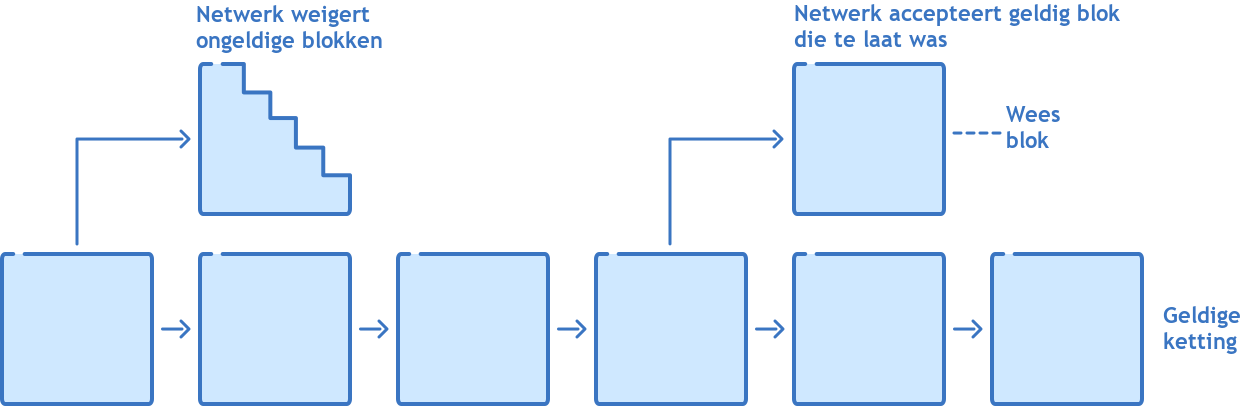
\includegraphics[width=\textwidth]{images/fig12.png}
    \caption{\footnotesize{\textit{Een kettingsplitsing is een natuurlijk proces dat optreedt wanneer miners tegelijkertijd een blok vinden tijd. De ketting die zwaarder wordt door totaal bewijs van werk is geldig, en de andere blok wordt wees.}}}
    \label{fig12}
\end{figure}



Het blok uit de VS wordt nu een zogenaamd wees-blok (\textit{orphan block}). Aangezien het alsnog werd verworpen, gaat de beloning voor de vinden verloren en de transacties uit dat blok worden niet in het grootboek geregistreerd. De verworpen transacties zijn niet verloren. Sommige werden misschien ook opgenomen in het blok uit China en de rest kan uiteindelijk in een toekomstig blok alsnog in het grootboek geschreven worden.

Alle onbevestigde transacties worden door miners lokaal bijgehouden op hun computer in een \textit{mempool}. Elke transactie uit een verworpen blok komt terug in de mempool terecht. Ze worden vervolgens door iemand anders in een blok geplaatst, zolang er geen conflict is met de nieuwe geschiedenis van het grootboek vastgelegd in het laatste blok.

Hoewel we in dit voorbeeld naar de \textit{nodes} refereren als zijnde Amerikaans of Chinese, weten nodes in realiteit niets over elkaars identiteit of geografische locatie. Het enige bewijs van validiteit dat ze nodig hebben, is dat iemand de zwaarste, cumulatieve proof-of-work ketting heeft en dat de transacties in die ketting zelf allemaal geldig zijn (geen dubbele-uitgaven).

Dit soort splitsingen van de ketting zijn vrij normaal en gebeuren af en toe in bitcoin. Doorgaans wordt opnieuw consensus bereikt in het volgend blok. Verbeteringen in technologie van bekendmaking van blokken en verhoogde netwerk-connectiviteit maken dit probleem mettertijd minder groot. Op vandaag, en hoogstwaarschijnlijk voor de nabije toekomst, heeft bitcoin een harde limiet op de hoeveelheid data dat toegelaten wordt in een blok. Een deel van de reden dat bitcoin, iedere tien minuten, relatief kleine blokken produceert, is om te verzekeren dat \textit{orphans} erg zeldzaam zijn.

Minen is een spel van kansen. Soms liggen blokken tien minuten uiteen, maar andere keren slechts enkele seconden. Indien we om de paar seconden blokken zouden produceren, of indien we erg grootte blokken zouden hebben, zou de kans groter zijn dat Amerikaanse en Chinese blokken conflicteren. Ze liggen ver uiteen en het duurt langer om elkaar te bereiken. Als \textit{orphans} te veel voorkomen, zou de ketting ontrafelen. We zouden \textit{orphan na orphan} zien verschijnen en \textit{nodes} zouden de tijd niet hebben om uit te maken welke nu het laatste, juiste blok is.

Het is belangrijk om blokken klein te houden om de kans te vergroten dat het hele netwerk de laatste blok kan ontvangen vooraleer te beginnen aan een volgende loterij. De andere, wellicht belangrijkste reden, is dat kleine blokken ook de vereisten qua hardware voor het draaien van een \textit{node} relatief laag houden. Zo blijft het de moeite om aan te sluiten bij het netwerk en blijft mining meer verspreidt over tijd. Grote blokken zouden miners aanzetten om zich te vestigen in \textit{datacenters} in gekende geografische locaties om splitsingen, die slecht zijn voor hun rendabiliteit, te vermijden

\section{De enige, echte ketting}
Laten we terugkeren naar ons voorbeeld uit hoofdstuk 3 waarin Henri voor het eerst aansluit bij het bitcoin netwerk.

De \textit{node} van Henri zal een connectie maken met enkele andere \textit{nodes} op het netwerk. Vervolgens vraagt hij die om nog andere \textit{nodes} die zij kennen en maakt ook daar verbinding mee. Dit heet \textit{node discovery}.

Sommige van die \textit{nodes} zullen slechte bedoelingen hebben en valse kopieën van het grootboek bezorgen. Ze kunnen bijvoorbeeld ongeldige handtekeningen voor transacties bevatten, of vervalste en oneerlijk ontgonnen bitcoin die geen geldige proof-of-work hashes hebben. Al die versies zullen onmiddellijk verworpen worden en de afzenders worden door de node van Henri verbannen.

Andere \textit{nodes} zullen wel eerlijk zijn, maar conflicterende versies van de waarheid hebben. Misschien ging een net offline en loopt hij nog enkele blokken achter. Wanneer hij verschillende kopieën van de blockchain download die allemaal geldig zijn, zal de software gebruik maken van Nakamoto Consensus. Door te meten wat het totale, cumulative proof-of-work is, weet Henri onmiddellijk welke de zwaarste ketting is die wordt aanzien als de enige echte.

\textit{Nodes} spreken voortdurend met elkaar om zeker te zijn dat ze het meeste recente blok hebben. Aangezien alle nodes de regel van de zwaarste ketting volgen, is er consensus over wat de ware staat van het grootboek is. Henri moet niet vertrouwen op een meerderheid van stemmen. Dit systeem zou makkelijk te bedriegen vallen door een grote hoeveelheid \textit{nodes} te draaien die kwaadaardig zijn.

Zelfs als Henri met verschillende verouderde of kwaadaardige nodes en slechts 1 correcte node connecteert, dan zou de bitcoin-software weten welke de juiste versie is. Die versie bevat de grootste hoeveelheid proof-of-work en bevat geldige transacties helemaal tot aan de \textit{genesis block}. Het belang hiervan kan niet genoeg benadrukt worden. Henri moet niemand vertrouwen; de software op zijn computer zal alle validaties uitvoeren die nodig zijn om zeker te zijn dat de \textit{blockchain} waar hij mee werkt de enige juiste is.

Het is daarom uiterst moeilijk voor hackers om een \textit{node} een valse kopie van de ketting te bezorgen. Om dat te doen zou je alle eerlijke connecties moeten kunnen uitsluiten en het doelwit enkel laten verbinding maken met je eigen, kwaadaardige \textit{nodes}.

\section{Omkeerbaarheid van transacties}
Doorgaans ontstaan concurrerende versies van het grootboek per toeval en wordt snel uitgeklaard welke de juiste versie is. Maar iemand die het netwerk wil aanvallen kan gebruik maken van Nakamoto Consensus door meer dan 50\% van de totale \textit{hash-rate} te beheren. Op die manier kunnen ze de zwaarste, cumulatieve proof-of-work ketting produceren. Die versie van het grootboek zal transacties bevatten die de aanvaller kiest, zolang ze genoeg energie willen verbruiken om de aanval door te zetten. Wanneer ze deze ketting bekendmaken aan het netwerk, zouden andere \textit{nodes} hem accepteren als zijnde de echte. Die heet een 51\%-aanval, omdat je meer dan de helft van alle rekenkracht op het netwerk nodig hebt om de aanval succesvol uit te voeren.

Het is belangrijk om te begrijpen dat er geen echte finaliteit van transacties is in bitcoin, aangezien 51\%-aanvallen of \textit{orphan blocks} altijd tot de mogelijkheid behoren. Ontvangers van transacties wachten typisch tot enkele blokken boven op hun transactie werd gemined. Wanneer de hoeveelheid energie die nodig zou zijn om de ketting te herschrijven hoog genoeg is, wordt het erg onwaarschijnlijk dat de transactie ongedaan wordt gemaakt en beschouwen de deze transfer als finaal.

Blokken die ontgonnen worden boven op een blok waar onze transactie in zit, noemen we doorgaans \textit{confirmaties}. Dus wanneer iemand zegt dat een bitcointransactie 6 confirmaties heeft, wordt bedoeld dat er 6 blokken gepasseerd zijn sinds de transactie in het grootboek zit. Wanneer je als handelaar een digitaal product verkoopt met geringe marginale kosten, kan het voldoende zijn met slechts 1 confirmatie of zelfs zonder confirmaties. Je stuurt de download link zodra de transactie aangekondigd werd op het netwerk. Wanneer je een huis verkoop, kan het misschien meer aangewezen zijn om te wachten op 12 confirmaties. Dat kost gemiddeld zo’n twee uur aan mining. Hoe langer je wacht, hoe meer proof-of-work boven op het blok met jouw transactie komt. Het wordt veel duurder om de transactie om te keren. Vandaag accepteren de meeste mensen een transactie met 6 confirmaties.

Moest de \textit{hash-rate} van bitcoin in belangrijke mate dalen, wat betekent dat minder energie ieder blok beveiligd, dan kan je altijd het aantal confirmaties verhogen vereist voor een “finale afwikkeling”. Hoewel de niet-finaliteit van transacties op het eerste zicht verontrustend lijkt, is het belangrijk om in het achterhoofd te houden dat transacties met kredietkaarten tot wel 120 dagen later kunnen worden teruggedraaid.

Aan de andere kant, zijn bitcointransacties na een paar blokken zo goed als onomkeerbaar. Vanuit dit oogpunt, is de omkeerbaarheid en finaliteit van bitcoin een ontzettende verbetering met de meeste traditionele betalingsnetwerken, althans voor de handelaar.

Op vandaag wordt geschat dat iemand met de energie van het volledige bitcoin netwerk ter beschikking – een serieuze uitdaging, aangezien je toegang tot de energie van een klein land én alle gespecialiseerde hardware moet hebben – nog altijd meer dan een jaar zou nodig hebben om de volledige geschiedenis van de \textit{chain} te herschrijven. Je kan deze data bekijken op \href{ https://bitcoin.sipa.be/}{ https://bitcoin.sipa.be/}

Footnote: dit interessante artikel gaat dieper in op ongeldige blokken in bitcoin: \href{ https://hackernoon.com/bitcoin-miners-beware-invalid-blocks-need-not-apply-51c293ee278b }{ https://hackernoon.com/bitcoin-miners-beware-invalid-blocks-need-not-apply-51c293ee278b }

\chapter{Forks en 51\%-aanvallen}
In de begindagen minede Satoshi zijn eerste bitcoins door gebruik te maken van de CPU in zijn computer. Aangezien de moeilijkheid oorspronkelijk erg laag was, bleek het relatief goedkoop om die munten te produceren.

Met tijd, begonnen mensen te sleutelen aan de software om te minen en werd het efficiënter. Uiteindelijk werd software geschreven die gebruik maakte van gespecialiseerde grafische apparatuur (GPU’s), gewoonlijk gebruikt door \textit{gamers}, om te minen.

Met GPU’s werd minen een heel stuk efficiënter. De moeilijkheidsgraad ging snel omhoog om de grote hoeveelheden \textit{hash-rate} van de GPU’s bij te benen. Minen met een CPU werd onrendabel.

Na de komst van GPU mining werd de efficientie van miners nog verhoogd door de product van \textit{Application Specific Integrated Circuits} (ASIC’s). Deze computerchips doen maar 1 ding: de bitcoin sha256 hash-functie uitvoeren. Ze kunnen enkel dit algoritme en bleken opnieuw een orde van grootte meer efficiënt dan GPU’s. De grafische kaarten voor gamers werden snel onrendabel om te minen, net zoals gebeurde met CPU’s. Iedere paar jaar komt een nieuwe generatie ASIC’s naar buiten die beter werken dan de vorige versies.

De eerste miners op het netwerk spendeerden slechts enkele centen aan elektriciteit om hun bitcoin te produceren. Terwijl de prijs omhoogging, en meer miners zich aansluiten bij het netwerk, ging de moeilijkheidsgraad van het minen omhoog en werd het duurder en duurder om bitcoins te produceren. Vandaag hangt de prijs rond de \$8.000 per BTC en spenderen miners duizenden dollars per geproduceerde bitcoin.

\section{Mining pools}
Een probleem met bitcoin mining is dat het niet-deterministisch is, zoals het rollen met een dobbelsteen. Dit betekent dat je een grote hoeveelheid geld kunt uitgeven aan elektriciteit en nooit een geldig blok vinden.

In 2010 werden zogenaamde \textit{mining pools} al populair om het probleem van variabiliteit te verbeteren. Een \textit{mining pool} is een manier om het risico te delen, vergelijkbaar met een verzekering.

Alle miners dragen bij aan een \textit{pool}. Het lijkt alsof ze 1 grote miner zijn op het netwerk. Wanneer iemand in die \textit{pool} een geldig blok vindt, wordt de beloning gedeeld met iedereen die bijdroeg, proportioneel verdeelt volgens de \textit{hash-rate} die ze bijdroegen. Dit stelt ook kleine mining-operaties in staat om beloningen te verdienen voor de kleine hoeveelheid rekenkracht die zij bijdragen. In ruil voor de dienst die zij aanbieden, nemen \textit{pool} een stukje van de beloning.

Het concept van \textit{mining pool} introduceerde enige centralisatie. Gebruikers sloten zich aan bij de grotere en bekendere diensten. Maar de gebruikers van de pools zijn wel eigenaar van hun \textit{hash-rate}. Ze kunnen op elk moment veranderen naar een nieuwe \textit{mining pool}.

Er bestaat historisch precedent voor individuele miners die een \textit{pool} verlaten omdat die te groot is geworden. In 2014 zat bijna de helft van de rekenkracht op het netwerk bij Ghash.io. De miners zagen in hoe gecentraliseerd dit werd en gingen vrijwillig over op andere diensten.

Hoewel de relatief gecentraliseerde mining pools vandaag een realiteit zijn, worden constant verbeteringen voorgesteld om de mining-technologie beter te maken, zoals bijvoorbeeld BetterHash. Met deze verbetering zouden individuele miners meer controle hebben over welke transacties ze precies willen minen, zonder hiervoor afhankelijk te zijn van coördinatie van hun \textit{mining pool}.

\section{51\%-aanvallen}
Centralisatie in \textit{mining pools} leidt tot bezorgdheid dat enkele van de grote pools zouden kunnen samenspannen om een 51\%-aanval uit te voeren op het netwerk. Vandaag hebben de vijf grootste identificeerbare pools meer dan 50\% van de totale mining \textit{hash-rate}. Laat ons onderzoeken hoe zo’n aanval wordt uitgevoerd en welke gevaren eraan verbonden zijn.

Wanneer je net meer dan 50\% van de rekenkracht in handen hebt, kan je de meerderheid van de toevoegingen aan het grootboek domineren. Je kan immers de zwaarste ketting produceren, mits je de aanval even kan volhouden. Herinner je dat Nakamoto Consensus stelt dat \textit{nodes} altijd de zwaarste cumulative proof-of-work \textit{chain} moeten accepteren die ze kennen.

Hier is een voorbeeld van een simpele 51\%-aanval:

\begin{enumerate}
\item Stel dat heel het netwerk bitcoin hasht aan 1000 hashes per seconde.
\item Je koopt een heleboel mining hardware en elektriciteit om 2000 hashes per seconde te produceren. We hebben nu 66\% van de totale \textit{hash-rate} (2000 van de 3000 hashes per seconde).
\item Je begint een ketting te minen met enkel lege blokken.
\item Binnen twee weken publiceer je de ketting van lege blokken. Omdat je veel sneller was dan de eerlijke miners, zal jouw versie twee keer zo veel proof-of-work bevatten. De aankondiging van jouw versie op het netwerk zal alle andere nodes doen overgaan op een \textit{reorg} waarin alle transacties uit de laatste 2 weken ongedaan worden gemaakt.
\end{enumerate}
Naast het minen van lege blokken, waardoor de \textit{chain} onbruikbaar wordt, is het ook mogelijk om een dubbele-uitgaven aanval uit te voeren:

\begin{enumerate}
\item Stuur bitcoin naar een handelsbeurs
\item Ruil om naar USD en haal de dollars af.
\item Op een later tijdstip kan je de\textit{ chain} publiceren zonder de transactie naar de handelsbeurs uit stap 1 hierboven.
\item Je herschreef de geschiedenis van het grootboek en bezit nu zowel de originele bitcoins als de dollars.
\end{enumerate}
De energieconsumptie van bitcoin’s \textit{hash-rate} is ongeveer equivalent met dat van een gemiddeld land. De benodigde hardware en elektriciteit verwerven om zo’n aanval uit te voeren is enorm duur. Schattingen tonen dat het ongeveer \$700.000 dollar per uur kost om een 51\%-aanval uit te voeren. Die kost blijft snel stijgen. Deze schatting neemt de reactie van eerlijke miners, wat de kost van de aanval nog zou opdrijven, niet in rekening.

Daarnaast is ook nog eens zeer moeilijk om een dubbele-uitgaven aanval succesvol af te ronden zonder vingerafdrukken achter te laten die duidelijk maken wie je bent. Tenslotte, je zou een hoeveelheid energie van een gemiddeld land aan het opgebruiken zijn, na miljoenen dollars aan hardware aan te kopen, en je moet een handelsbeurs vinden waar je miljoenen dollars kan uitcashen om de aanval te doen slagen.

Maar stel dat een kwaadaardige partij, met ongelimiteerde budgetten, zoals een overheid, zou beslissen om dit te doen en erin slaagt om de aanval vol te houden zodat het effect op het netwerk meer dan gewoon wat overlast is. Dan nog zou het netwerk in principe kunnen reageren door de proof-of-work functie te veranderen (naar iets anders dan sha256). Hierdoor zou alle bestaande bitcoin mining hardware, die de aanvaller ook gebruikt, nutteloos worden. Die machines dienen specifiek om sha256 hashes te doen. Maar het aanpassen van het proof-of-work algoritme moet je zien als een laatste redmiddel en alle eerlijke miners zouden eveneens in de klappen delen. Toch zou het netwerk overleven.

Naast de onwaarschijnlijkheid van de aanval, geeft het hebben van de meerderheid van de \textit{hash-rate} je nog altijd het recht niet om dingen te doen die nog belangrijker zijn:

\begin{enumerate}
    \item Je kan geen munten uit het niets creëren die de regels van uitgifteschema schenden. Aangezien dit de consensusregels van de blokbeloning zou overtreden, worden de blokken gewoon verworpen, zelfs al hadden ze genoeg proof-of-work.
    \item Je kan geen munten uitgeven die niet van jou zijn. Het is onmogelijk om een geldige digitale handtekening hiervoor te leveren.
\end{enumerate}

De nodes die bitcoin accepteren voor betalingen zouden het netwerk eerlijk houden in het aanzicht van een oneerlijke meerderheid van miners door simpelweg de regels van bitcoin toe te passen. Aldus is een 51\%-aanval eerder hinderlijk dan een veiligheidsrisico. Waarschijnlijk is het \textit{worst-case scenario} hier dat een overheid met een goed gevulde portemonnee, bitcoin probeert onbruikbaar te maken. Maar zo’n aanval kan niet eeuwig duren. Wanneer bitcoin herstelt van een aanval zoals beschreven, zou het enkel haar veerkracht benadrukken en een nog groter probleem worden voor zij die het willen aanvallen.

Hoewel bitcoin tot dusver nog nooit met succes aangevallen is met een 51\%-aanval, hebben we wel voorbeelden van andere \textit{blockchain} die veel minder hash-rate hebben die hen beveiligd. In deze gevallen waren de beurzen het slachtoffer van de aanval en verloren ze geld aan munten met lage hash-rate die ze in de eerste plaats nooit hadden moeten aanbieden op hun platform.



\chapter{Accounts zonder identiteit}

We hebben nu een gedistribueerd grootboek gebouwd zonder centrale autoriteit, een loterij om te bepalen wie erin mag schrijven, een systeem om eerlijke miners te belonen en valsspelers te straffen, een manier om de moeilijkheidsgraad aan te passen om een consistent uitgifteschema te garanderen en conflicten te verminderen en een systeem om de geldigheid van de keten te controleren door te kijken naar het cumulatieve \textit{proof-of-work} en de transactiegeschiedenis.

Laten we nu eens kijken naar identiteit. Om in een traditioneel banksysteem geld te versturen moet je eerst jezelf identificeren bij de bank. Je geeft je identiteit (je bankpas) en pincode in bij de geldautomaat, of typt je gebruikersnaam en wachtwoord in een mobiele app. De bank zorgt ervoor dat entiteiten niet dezelfde identiteit delen.

Hoe kunnen we in ons nieuwe op bitcoin gebaseerde financiële systeem een rekening openen zonder een centrale partij die de identiteiten bijhoudt? Hoe kunnen we onze identiteit loskoppelen van financiële transacties, zodat identiteitsdiefstal voorkomen wordt en we niemand hoeven te vertrouwen met onze informatie? Hoe zorgen we ervoor dat wanneer Alice aankondigt Bob te willen betalen, we kunnen garanderen dat zij het echt is en dat ze de bevoegdheid heeft om dat geld te verplaatsen?

\section{Een bitcoinrekening aanmaken}

In ons systeem bestaat geen centrale tussenpersoon (zoals een bank) om alle rekeninghouders te registreren. Wat als we iedereen zijn eigen gebruikersnaam en wachtwoord laten kiezen? Doorgaans controleert een bank of een gebruikersnaam al bestaat, maar dat is in ons geval onmogelijk aangezien er geen centrale partij is om nieuwe identiteiten uit te geven. Een gebruikersnaam en wachtwoord zijn in ons geval niet voldoende. We zullen opnieuw een techniek moeten gebruiken die we al kennen uit eerdere hoofdstukken, namelijk gigantische willekeurige getallen. 

Door grote willekeurige getallen te genereren, kan iedereen loten kopen om mee te spelen met de loterij. We kunnen hetzelfde doen om rekeningen aan te maken. Om een bitcoinrekening, of \textit{adres}, aan te maken, zullen we eerst twee 256-bits getallen genereren die wiskundig aan elkaar gekoppeld zijn --- een \textit{publiek/privé-sleutelpaar}. Herinner dat een 256-bits getal ongeveer even groot is als het aantal atomen in het heelal, dus twee mensen die per ongeluk hetzelfde sleutelpaar genereren is haast onmogelijk. We geven ons adres aan iedereen die ons geld wil sturen. We gebruiken de privésleutel om het geld weer uit te geven. Dit is hoe het werkt.

Versleuteling is een methode om leesbare tekst om te zetten naar geheimschrift, zodat alleen iemand die de sleutel heeft het originele bericht kan lezen door de versleuteling weer ongedaan te maken. Als kinderen speelden sommigen van ons al met speelgoed waar een enkele sleutel nodig was om een bericht in wartaal te veranderen, om het even later met dezelfde sleutel weer te ontsleutelen. Dit soort codering wordt symmetrisch genoemd. Een systeem met een publiek/privé-sleutelpaar is \textit{asymmetrisch}, omdat je met de ene sleutel kunt versleutelen en de andere moet gebruiken om weer te ontsleutelen.

De publieke sleutel kan je naar believen met de hele wereld delen. Mensen die je berichten willen sturen kunnen ze versleutelen met je publieke sleutel, en omdat alleen jij de privésleutel bezit, ben jij de enige die de berichten kan decoderen.

Laten we eens kijken hoe Alice munten naar Bob stuurt. Om een transactie te ontvangen genereert Bob een sleutelpaar en houdt hij zijn privésleutel geheim. Hij genereert een \textit{adres}; een lange reeks van cijfers en letters op basis van een hash van zijn publieke sleutel. Bob deelt dit adres vervolgens met Alice.

Vergelijk dit adres met een brievenbus. In plaats van brieven kan Alice munten in deze brievenbus laten vallen. Maar alleen Bob heeft de privésleutel die nodig is om de brievenbus te openen en de munten te besteden.

Wanneer je geld op de bank zet, geef je ze je gebruikersnaam en wachtwoord. Wanneer je cheques uitschrijft, onderteken je met je naam om te verifiëren dat jij het bent die de cheque uitschrijft. Wanneer je bitcoins wilt verplaatsen, toon je bewijs dat je de sleutel bezit van het adres waar de munten bij horen.

Alice moet bewijzen dat ze de privésleutel van haar publieke sleutel heeft. Ze wil haar privésleutel echter niet blootstellen aan hackers omdat ze dan haar munten uit haar brievenbus kunnen stelen.

Alice's bewijs van sleutelbezit wordt een \textit{digitale handtekening} genoemd. Alice construeert een transactie die er ongeveer zo uit ziet:

\begin{verbatim}
Adres 12345 met 2,5 bitcoins 
verstuurt 2 bitcoins naar adres 56789 en 
stuurt 0.5 bitcoins terug naar adres 12345
\end{verbatim}

In werkelijkheid zijn de adressen gigantische 160-bits getallen. Zij versleutelt vervolgens dezelfde transactie met haar privésleutel en genereert daarmee een \textit{digitale handtekening}.

Wanneer ze haar transactie publiceert naar de andere nodes op het netwerk, onthult ze de publieke sleutel van de brievenbus van waaruit ze verzendt, en de digitale handtekening die ze met haar privésleutel heeft gegenereert. Alice kondigt het volgende aan:

\begin{itemize}
    \item Ik stuur munten vanaf adres 12345
    \item Hier is de publieke sleutel voor adres 12345. Je zult zien dat als je de publieke sleutel hasht, je hetzelfde adres zult verkrijgen.
    \item Hier is een handtekening die ik heb versleuteld met de privésleutel die correspondeert met dit adres. Je kunt de publieke sleutel gebruiken om deze te ontsleutelen en controleren of het overeenkomt met mijn transactiedata.
\end{itemize}

\begin{figure}
    \centering
    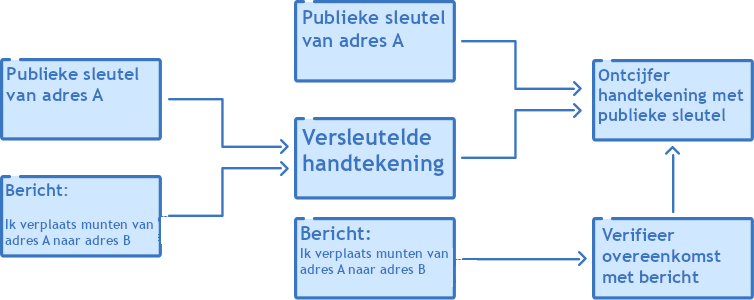
\includegraphics[width=\textwidth]{images/fig13.png}
    \caption{\footnotesize{\textit{Er wordt een digitale handtekening gegenereert door de transactie te versleutelen met de privésleutel. Dit kan worden ontsleuteld met behulp van de openbare sleutel, die bij iedereen bekend is.}}}
    \label{fig13}
\end{figure}

Aangezien iedereen nu de publieke sleutel van de brievenbus van Alice heeft, kan de digitale handtekening eenvoudig worden ontsleuteld. Als de handtekening kan worden ontsleuteld met de publieke sleutel van het adres, weet iedereen dat Alice in het bezit moet zijn van de bijbehorende privésleutel. Ontsleutelen was anders niet mogelijk geweest, omdat de publieke sleutel alleen berichten kan ontsleutelen die zijn versleuteld met de bijbehorende privésleutel. Het is belangrijk om hierbij op te merken dat niemand haar privésleutel heeft gezien, maar wél het bewijs dat ze over de juiste privésleutel beschikt om haar handtekening te zetten.

In tegenstelling tot je pincode of een handtekening op een cheque, is een digitale handtekening specifiek voor de unieke transactiegegevens die je ondertekend. De handtekening kan dus niet worden gestolen en opnieuw worden gebruikt voor een andere transactie. Elke transactie krijgt een andere handtekening, zelfs als deze wordt verzonden vanaf de hetzelfde publieke adres, met dezelfde privésleutel, aangezien alle nieuwe gegevens de handtekening wijzigen.


\section[Kan je een privésleutel raden?]{Kan je een privésleutel raden?}

Laten we eens kijken hoe groot de kans is om een privésleutel te raden, wat je de mogelijkheid zou geven om munten te verplaatsen van het bijbehorende publieke adres. Onthoud dat een sleutel uit 256-bits bestaat. Elke bit heeft slechts twee waarden (een of nul). Dat betekent dat je elk bit kunt visualiseren als het opgooien van een muntje.

Een privésleutel van 1 bit is alsof we een munt opgooien. Kop of munt, één of nul? Je hebt een kans van één op twee om het goed te raden.

Basis statistiek: de kans op verschillende gebeurtenissen wordt berekend door de individuele kans van elke gebeurtenis met elkaar te vermenigvuldigen. Als een munt $1/2$ kans heeft om kop te landen, dan is de kans om twee keer op rij kop te gooien $1/2 \times 1/2 = 1/4$ of 1 op 4.

Als je de uitkomst van 8 munten op een rij zou moeten raden is dat $2^{8}$; een kans van één op 256.

Een kentekenplaat heeft 6 letters en cijfers. Er zijn 26 letters en 10 cijfers, dus in totaal 36 tekens. Het aantal mogelijke kentekenplaten is dus $36^{6}$, en je kans om de mijne te raden is dus een op de twee miljard.\footnote{De inspiratie voor dit gedeelte kwam van een uitstekende Medium post die de waarschijnlijkheid van een aantal gebeurtenissen in detail beschrijft. Ik raad aan de volledige post te lezen voor de context: \href{https://medium.com/@kerbleski/a-dance-with-infinity-980bd8e9a781}{https://medium.com/@kerbleski/a-dance-with-infinity-980bd8e9a781}}

Een kredietkaart bestaat uit zestien cijfers. Ieder cijfer heeft 10 verschillende mogelijkheden, dus je kans om mijn kredietkaart te raden is $10^{16}$, dat is één op 10.000.000.000.000.000 of ongeveer één op tien quadriljoen.

Er zijn ongeveer $10^{50}$ atomen op aarde. Als ik aan een willekeurig atoom denk, is jouw kans om die te raden ongeveer

\begin{verbatim}
    Één op 1.000.000.000.000.000.000.000.000.
    000.000.000.000.000.000.000.000.000.
\end{verbatim}

Een privésleutel heeft 256 bits, wat gelijk is aan $2^{256}$ of ongeveer $10^{77}$. En daarmee is de kans om mijn volledige privésleutel correct te raden kleiner dan de kans op het raden van een specifiek atoom in het universum, of de kans om 10 keer achter elkaar de jackpot van de Staatsloterij te winnen.

Maar wat nou als een super krachtige computer al het gokwerk voor je zou kunnen doen? Dit wordt het best uiteengezet in de Redditpost op https://bit.ly/2Dbw9Qd en ik raad het je aan om hem in zijn volledigheid te lezen. Hij is wellicht wat technisch, maar de laatste paragraaf geeft je een goed beeld wat er voor nodig is om alle mogelijke 256-bits sleutels te noteren: 

\begin{quotation}
Dus, als je de volledige planeet als harde schijf zou kunnen gebruiken, 1 byte per atoom zou kunnen opslaan, de sterren gebruikt als brandstof om je langs 1000 miljard sleutels te fietsen, dan heb je 37 octiljoen ($10^{48}$) keer de aarde nodig voor opslag, en 237 miljard keer de zon om je apparaat van brandstof te voorzien, waar je alles te samen 3.6717 octodeciljoen  ($10^{57}$)  over zult doen\par\raggedleft--- \textup{u/PSBlake, R/Bitcoin}
\end{quotation}

Het is dus praktisch onmogelijk om iemands privésleutel te raden. Dat niet alleen; het aantal mogelijke bitcoinadressen is zo groot, dat het aan te raden is om voor iedere transactie een nieuw adres met een nieuwe privésleutel te genereren. Dus in plaats van een enkele bankrekening, zou je zo maar eens over duizenden of zelfs miljoenen bitcoin accounts kunnen beschikken. Namelijk 1 voor iedere transactie die je ooit hebt ontvangen.

Het is misschien verontrustend dat je bitcoin account slechts beveiligd is door toeval, maar hopelijk helpt de verklaring hierboven je om te beseffen dat dit vele malen veiliger is dan de pincode tot je bankrekening, opgeslagen op een centrale server, en een eenvoudig doel voor hackers.

\section{Het saldo monitoren}

Het wordt tijd om een laatste leugentje van de voorgaande hoofdstukken te corrigeren. Er worden namelijk geen saldi bijgehouden op de blockchain. In plaats daarvan maakt bitcoin gebruik van zogeheten UTXO: Unspent Transaction Outputs. De transactie output is simpelweg een woord voor de muten die je in een vorige transactie hebt ontvangen, ongeacht of je ze van iemand ontvangen hebt of door het minen hebt verkregen in de \textit{coinbase transactie}.

Bitcoins zijn deelbaar in 100 miljoen eenheden die we satoshis noemen. Dit in tegenstelling tot de metalen munten die vaak alleen in vooraf gespecificeerde eenheden voorkomen, zoals we bijvoorbeeld de 10 cent, twintig cent en euro muntstukken kennen. Daarom zul je soms munten van verschillende adressen met elkaar moeten combineren, of juist een grotere UTXO in tweeën moeten splitsen, om ze naar iemand anders te sturen. Zie het als het sturen van een stapel munten naar een machine die ze omsmelten en nieuwe munten maken van elke waarde die u wilt. Portefeuilles, die later in dit hoofdstuk worden besproken, beheren dit over het algemeen allemaal achter de schermen, zodat u alleen het bedrag hoeft op te geven dat u wilt verzenden.

Laten we zeggen dat Alice een adres heeft dat 1 bitcoin bevat. Ze wil 0,3 bitcoins naar Bob sturen. Ze genereert een transactie die haar adres toont met een 1 bitcoin UTXO als input en twee outputs: een nieuwe bitcoin UTXO ter waarde van 0.3 naar Bob's adres, en een nieuwe bitcoin UTXO ter waarde van 0.7 terug naar haar eigen adres als wisselgeld. Het wisselgeld kan naar haar oorspronkelijke verzendadres gaan, of voor een betere privacy kan ze het naar een nieuw adres sturen dat ze ter plekke genereert.

\begin{figure}
    \centering
    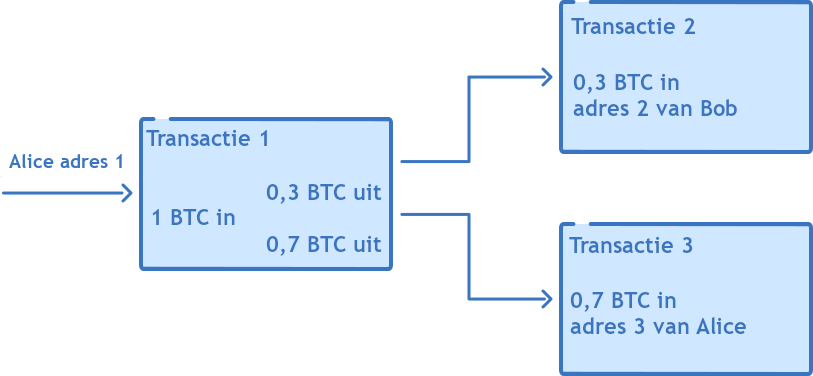
\includegraphics[width=\textwidth]{images/fig14.png}
    \caption{\footnotesize{\textit{Als je geen UTXO hebt in het exacte bedrag dat je wilt sturen, dan zal er een worden gesplitst om wisselgeld te maken. Je kunt ook verschillende UTXO's combineren om een nieuwe grotere te maken.}}}
    \label{fig14}
\end{figure}

Er is geen manier in de keten om te vertellen wie welk adres controleert. Daarvoor zou je de corresponderende private sleutels moeten kennen en ze moeten koppelen aan echte identiteiten. Het UTXO-model moedigt een zeer mooi privacymechanisme aan door bij elke muntverplaatsing het wisselgeld naar een nieuw adres te sturen. Zo kan een persoon honderden of duizenden adressen bezitten als hij vele malen munten heeft verzonden of ontvangen. De software van de portemonnee beheert dit alles voor ons, zodat we ons geen zorgen hoeven te maken over de details.

Dus, om het saldo van een bepaald adres te controleren, moeten we eigenlijk alle UTXO's optellen die dit adres als uitgang hebben. De totale set van huidige UTXO's in bitcoin groeit wanneer mensen van één adres naar veel adressen sturen, en krimpt wanneer mensen consolidatietransacties uitvoeren waarbij munten van veel adressen aan één adres worden uitgegeven.

Het UTXO-model maakt een eenvoudige en efficiënte validatie van dubbele uitgaven mogelijk, omdat een bepaalde UTXO maar één keer kan worden uitgegeven. Wij hoeven niet de hele geschiedenis van uitgaven van een bepaalde rekening te kennen.

We kunnen ook een willekeurig aantal UTXO's tegelijk creëren en vernietigen, waardoor complexe transacties ontstaan die verschillende inputs en outputs mixen. Dit maakt het idee van CoinJoin\footnote{\href{https://en.bitcoin.it/wiki/CoinJoin}{https://en.bitcoin.it/wiki/CoinJoin}} mogelijk, waarbij verschillende partijen deelnemen aan een enkele bitcoin-transactie die een willekeurig aantal inputs mengt om een willekeurig aantal outputs te produceren, en zo de geschiedenis van de UTXO's versluiert. De populariteit van dergelijke technieken neemt toe en is belangrijk voor de privacy en fungibiliteit, een term die zegt dat elke bitcoin gelijkwaardig is aan elke andere bitcoin. Op die manier, als sommige bitcoins in de handen van onfrisse partijen terechtkomen, zijn ze niet voor eeuwig bezoedeld alleen maar omdat ze een keer voor iets snode zijn gebruikt.

\section{Wallets}

Een account aanmaken is niets meer dan een willekeurig 256 bit sleutelpaar aanmaken. We kunnen duizenden of miljoenen accounts aanmaken, dus hebben we een manier nodig om ze te traceren. In bitcoin wordt het woord portemonnee gebruikt om te verwijzen naar elk soort apparaat dat uw sleutels bijhoudt. Dat kan zo simpel zijn als een stuk papier of zo complex als een stuk hardware. 

De originele bitcoin-code die door Satoshi werd gepubliceerd, werd geleverd met een software-portemonnee. Deze portemonnee genereerde uw adressen voor u, sloeg uw sleutels op en selecteerde UTXO's voor u om uit te geven, zodat u gemakkelijk bitcoins van elke waarde kon versturen. 

In tegenstelling tot de portemonnee van uw bank, die meestal de vorm heeft van een mobiele of webapplicatie die door uw bank is gemaakt, is bitcoin een volledig open systeem. Daarom zijn er tientallen portemonnees, waarvan de meeste gratis zijn, en veel ook open source, evenals een half dozijn implementaties van hardware-portemonnees en er komen er nog meer. Iedereen met kennis van computerprogrammering kan zijn eigen portemonnee bouwen of de code van een open source portemonnee lezen om er zeker van te zijn dat er niets vals aan de hand is. 

Omdat je private key het enige is dat je nodig hebt om je munten uit te geven, moet je die goed bewaken. Als iemand uw kredietkaart steelt, kunt u het bedrijf bellen en een fraudeklacht indienen en proberen uw geld terug te krijgen. Bij bitcoin is er geen tussenpersoon. Als iemand uw privésleutel heeft, heeft hij uw munten in handen, en er is niemand die u kunt bellen. 

Prive-sleutels zijn ook gevoelig voor verlies. Als u uw portemonnee op uw computer bewaart en de computer wordt gestolen of vliegt in brand, dan heeft u een probleem. Als u de beste bitcoin-praktijken volgt en elke keer dat u betalingen ontvangt een nieuw adres genereert, wordt het veilig opslaan en back-uppen van deze privésleutels al snel een lastige zaak. 

In de loop der tijd heeft het bitcoin-ecosysteem een aantal oplossingen voor dit probleem ontwikkeld. In 2012 werd BIP32 (Bitcoin Improvement Proposal, een mechanisme voor mensen om ideeën te verspreiden over hoe bitcoin verbeterd kan worden) voorgesteld om Hierarchical Deterministic Wallets te maken. Het idee hierachter is dat we met slechts één willekeurig getal, een se d genaamd, continu vele sleutelparen kunnen genereren die bitcoinadressen en privésleutels voor hen vertegenwoordigen. 

Als u tegenwoordig een van de algemeen beschikbare software- of hardware-portemonnees gebruikt, genereert deze automatisch nieuwe sleutels voor u voor elke transactie, zodat u slechts één hoofdsleutel hoeft te back-uppen. 

In 2013 kwam BIP39 om het back-uppen van sleutels nog eenvoudiger te maken. In plaats van een willekeurig getal te gebruiken, zouden sleutels worden gegenereerd uit een willekeurige set van door mensen leesbare woorden. Hier is een voorbeeld van een seed:

\begin{verbatim}
    witch   collapse    practice    feed
    shame   open        despair     creek
    road    again       ice         least
\end{verbatim}

Met deze methode werd het back-uppen van sleutels heel eenvoudig: je kon het zaad op een stuk papier schrijven en het in een kluisje stoppen. Je zou de zin zelfs uit je hoofd kunnen leren en uit een falend economisch regime als Venezuela weg kunnen lopen zonder iets bij je te hebben, zonder dat iemand er iets van merkt dat je je rijkdom in je hoofd meedraagt. 

Bovendien kan een bitcoin-adres meer dan één privé-sleutel vereisen om toegang te krijgen. Adressen met verschillende handtekeningen of multisig-adressen kunnen een grote verscheidenheid aan beveiligingssystemen gebruiken. Twee mensen kunnen bijvoorbeeld een rekening delen met 1-of-2 multisig, waarbij elke partij kan tekenen voor transacties en munten kan uitgeven. 

Een 2-of-2 multisig die vereist dat beide partijen sleutels leveren om uit te geven kan worden gebruikt om te voorkomen dat een enkele persoon controle krijgt over een rekening, bijvoorbeeld tussen zakenpartners. 

Je kunt een eenvoudig escrow-systeem maken met een 2-van-3 multisig. De koper krijgt een sleutel, de verkoper krijgt een andere sleutel, en een derde sleutel wordt aan een arbiter gegeven. Als koper en verkoper het eens zijn, kunnen ze samen de fondsen deblokkeren. In het geval van een geschil kan de arbiter samen met een van de partijen optreden om de fondsen te deblokkeren. 

U kunt een 3-of-5 multisig schema gebruiken om uzelf te beschermen tegen het verlies van sleutels door uzelf toe te staan maximaal 2 van de 5 sleutels te verliezen en nog steeds in staat te zijn de rekening te deblokkeren. U kunt twee van de sleutels op verschillende plaatsen bewaren, twee bij verschillende betrouwbare vrienden die elkaar niet kennen, en één bij een gespecialiseerde bewaardienst zoals BitGo die uw transacties mede ondertekent, waardoor uw bitcoin zeer moeilijk te stelen is terwijl u uzelf beschermt tegen het verlies van sleutels. 

U kunt zelfs nog verder gaan en adressen maken die ontgrendeld worden door vrij complexe voorwaarden met behulp van programmeerconstructies zoals voorwaardelijke verklaringen ("als dit, dan dat"). Je zou zelfs munten kunnen opsluiten in een adres dat pas over 10 jaar toegankelijk is, en zelfs jij als maker van zo'n adres kunt niet van gedachten veranderen en de code veranderen om die munten voor die tijd uit te geven. 

Er komen steeds meer semi-custodiale oplossingen van bedrijven zoals Casa en Unchained Capital, die u helpen om sleutels op een veilige manier op te slaan. In tegenstelling tot een bank, die je rekening kan bevriezen, fungeren deze oplossingen voor gedeeltelijke bewaring als een back-up of vertrouwde medeondertekenaar, maar kunnen ze zelf je fondsen niet meenemen zonder je sleutels. Portefeuillesoftware evolueert voortdurend omdat daarvoor niemands toestemming nodig is, in tegenstelling tot de app van je bank. Daarom zien we steeds meer nieuwe toetreders en meer innovatie. 

Dit is ingrijpend en wereldveranderend. Nooit eerder was het mogelijk om je vermogen bij je te dragen op een manier die volledig veilig is tegen inbeslagname of diefstal. 





\chapter{Wie bepaalt de regels?}

We hebben nu een functioneel en gedistribueerd systeem om waarde te volgen en te verplaatsen. Laten we eens kijken wat we zover hebben gebouwd:

\begin{enumerate}
    \item Een gedistribueerd grootboek, waarvan iedere deelnemer een kopie bewaard.
    \item Een loterij-systeem gebaseerd op proof-of-work en aanpassingen in moeilijkheidsgraad om het netwerk te beveiligen tegen gesjoemel en het uitgifteschema consistent te houden.
    \item Een consensussysteem waarmee iedere deelnemer zelfstandig in staat is om de volledige geschiedenis van de blockchain te valideren door gebruik te maken van open source software genaamd de bitcoin client. 
    \item Een identificatiesysteem met digitale handtekeningen waarmee naar willekeur een account-achtige mailbox kan worden gecreëerd voor de ontvangst van munten, zonder tussenkomst van een centrale autoriteit.
\end{enumerate}

Nu is het tijd om een van de meest interessante en contra-intuïtieve zaken van bitcoin te tackelen. Waar komen de regels vandaag, hoe worden ze afgedwongen en hoe kunnen ze over tijd veranderen. 

\section{Bitcoin-software}

In de vorige hoofdstukken gingen we ervan uit dat iedereen op het netwerk dezelfde regels valideert: ze verwerpen dubbele betalingen, controleren ieder blok op proof-of-work, of ieder blok verwijst naar het vorige blok, en of iedere transactie in ieder blok correct is ondertekend door de eigenaar van het adres, naast een veelvoud aan andere zaken waar men het in de loop der tijd over eens is geworden. 

We hebben ook gezegd dat bitcoin open source software is. Open source betekent dat iedereen de code kan lezen, maar ook dat iedereen zijn eigen kopie kan wijzigen. Hoe komen dergelijke wijzigingen in bitcoin?

Bitcoin is een \textit{protocol}. In computersoftware verwijst deze term naar een set regels die door de software worden gehanteerd. Zolang je binnen de regels blijft, staat het je vrij om de software naar wens te wijzigen. Als we het hebben over mensen die "bitcoin nodes runnen," bedoelen we in feite dat ze software draaien die zich aan het bitcoin protocol houden. Deze software kan met andere bitcoin nodes communiceren, transacties en blokken doorgeven, andere nodes ontdekken om mee te verbinden, enzovoorts.   

De daadwerkelijke implementatie van het bitcoinprotocol is aan de gebruiker. Er zijn vele verschillende implementaties van het bitcoinprotocol. De populairste is Bitcoin Core, een uitbreiding van het werk dat door Satoshi Nakamoto werd vrijgegeven.

Er zijn ook andere implementaties, in andere computertalen en onderhouden door andere mensen. Consensus is een essentieel onderdeel van bitcoin. Om ervoor te zorgen dat de consensus in bitcoin behouden blijft, draait het grootste gedeelte van de nodes dezelfde Bitcoin Core software. Zo worden incidentele bugs voorkomen die er anders voor zouden kunnen zorgen dat nodes het niet langer eens zijn welke blokken geldig of juist ongeldig zijn. In feite is er geen enkele volledige specificatie van het bitcoinprotocol, dus de beste manier om nieuwe bitcoin client software te ontwikkelen is om de originele code te lezen en te zorgen dat je er niet te veel vanaf wijkt, zelfs als het een aantal fouten bevat.

\section{Wie maakt de regels?}

De regels die bitcoin vormgeven staan gecodeerd in de Bitcoin Core client. Maar wie bepaalt deze regels? Waarom zeggen we dat bitcoin schaars is als iemand zomaar het limiet kan wijzigen van 21 naar 42 miljoen?

In een gedistribueerd systeem, moeten alle nodes overeenstemmen over de regels. Als jij als miner besluit om de software zo te wijzigen dat je jezelf twee keer zoveel mag belonen bij het minen van een blok dan volgens het huidige beloningsschema is toegestaan, dan zal iedere andere node in het netwerk je blok weigeren. Het wijzigen van de regels is extreem lastig omdat je de duizenden nodes wereldwijd moet overtuigen om de nieuwe regels te hanteren.

Bitcoins bestuursmodel is contra-intuïtief, met name voor mensen uit onze westerse democratie. We zijn gewend om op basis van stemmen te besturen -- de meerderheid van mensen kan bepalen, een wet doorvoeren, en hun wil opleggen aan de minderheid. Bitcoins bestuursmodel ligt veel dichter bij anarchie dan bij democratie.

Iedereen die bitcoin-betalingen accepteert, bepaalt voor zichzelf wat zij als bitcoin beschouwen. Als iemand software draait die zegt dat er 21 miljoen bitcoins zijn, en u probeert hen bitcoins te sturen geproduceerd door uw malafide software die deze limiet negeert, zullen uw munten als vals worden gezien en worden geweigerd.

Laten we eens kijken naar de verschillende deelnemers in de bitcoinwereld en hoe ze elkaar in evenwicht houden:

\paragraph{}
\noindent\textbf{Nodes:} 
Iedere deelnemer in het bitcoinnetwerk runt een node en bepaalt zelf welke software hierop draait. De meeste mensen gebruiken Bitcoin Core. Dit is de implementatie van het bitcoinprotocol die door Satoshi in het leven werd geroepen en verder is doorontwikkeld door honderden onafhankelijke ontwikkelaars en bedrijven van over de hele wereld. Mocht deze software implementatie kwaadaardig blijken, bijvoorbeeld door inflatie te introduceren, dan zal geen enkele node-operator het nog langer draaien. Nodes worden onder andere gedraaid door iedereen die bitcoin accepteert: Handelaren, Exchanges, Wallet-aanbieders, en mensen zoals jij en ik die bitcoin gebruiken voor welke reden dan ook. 

\paragraph{}
\noindent\textbf{Miners:} 
Sommige van deze nodes minen ook; ze brengen nieuwe bitcoin in omloop, nemen transacties op en zorgen ervoor dat het erg kostbaar wordt om het grootboek te manipuleren. Je zou de miners kunnen beschouwen als de enige regelgevers omdat zij de enige zijn die in het grootboek schrijven, maar dat zijn ze niet. Ze volgen de regels die worden bepaald door de nodes die bitcoin accepteren. Zodra miners blokken produceren waarin bijvoorbeeld een extra beloning is opgenomen, dan worden deze verworpen door de andere nodes, met als gevolg dat de extra beloning geen waarde meer vertegenwoordigd. Dus kan je stellen dat iedere gebruiker met een node onderdeel is van een anarchisch overheidsmodel - zij bepalen aan welke regels de munten die zij als bitcoin beschouwen moeten voldoen, en iedere overtreding van deze regels wordt direct afgewezen.

\paragraph{}
\noindent\textbf{Gebruikers / Investeerders:} 
Gebruikers zijn de mensen die (de valuta) bitcoin kopen en verkopen. Lang niet alle gebruikers runnen hun eigen node, maar vertrouwen op de node van een derde partij, bijvoorbeeld de aanbieder van hun portemonnee, waar deze aanbieder fungeert als soort van proxy voor de wensen en verlangens van hun gebruikers. Gebruikers bepalen de waarde van de munt op de open markt door vraag en aanbod. Als de miners en handelsbeurzen zouden samenspannen om zoiets radicaals als inflatie te implementeren, dan zou de markt de munt die deze nieuwe regels zou volgen waarschijnlijk verwerpen, de prijs zou dalen en de bedrijven al snel zonder werk komen te zitten. Een intolerante minderheid kan de originele munt dus altijd zelfstandig in leven houden.

\paragraph{}
\noindent\textbf{Ontwikkelaars:}
De Bitcoin Core software is het meest populaire bitcoin client project. Het heeft een rijk ecosysteem van honderden 's werelds beste crypto ontwikkelaars en bedrijven aan weten te trekken. Het Bitcoin Core project is uitermate conservatief omdat de software een netwerk draaiende houdt dat ondertussen meer dan \$1000 miljard aan waarde vertegenwoordigd. Ieder idee voor grootschalige verandering doorloopt een proces genaamd Bitcoin Improvement Proposal (BIP) \footnote{Lees meer over Bitcoin Core's ontwikkelingsprocess in \href{https://blog.lopp.net/who-controls-bitcoin-core-/}{blog.lopp.net/who-controls-bitcoin-core-/}} en iedere verandering in de code wordt nauwkeurig beoordeeld door collega-ontwikkelaars. Het verbeterproces en de code review is volledig transparant en publiek. Iedereen mag meedoen, commentaar geven of wijzigingen in de code voorstellen. Als bepaalde ontwikkelaars corrupt worden en software ontwikkelen die niemand wil draaien, dan kan een gebruiker simpelweg zelf bepalen om andere software te draaien, een oudere versie te hanteren of besluiten om zelf iets nieuws te beginnen. Hierdoor zijn core developers min of meer gedwongen om veranderingen door te voeren die naar wens is van de gebruikers, anders lopen ze het risico om de status van referentie-implementatie te verliezen. 

\section{Een splitsing van de regels (Forks)}

Als het goed is begrijp je nu hoe bitcoin software de afgesproken regels handhaaft en dat mensen zelf mogen bepalen welke software ze willen draaien om de regels af te dwingen waar ze in geloven.

Miners bepalen zelf welke regels ze hanteren als ze blokken produceren, maar zijn gedwongen om hierbij te luisteren naar de wens van de gebruikers. Doen ze dit niet, dan worden de blokken niet geaccepteerd en riskeren ze de blokbeloning.

We weten inmiddels ook dat bitcoin software de blockchain met het meeste proof-of-work accepteert als de enige ware keten en dat er af en toe een splitsing (een zogeheten fork) ontstaat omdat er bij toeval gelijktijdig een blok wordt geproduceerd.

Door de grote verscheidenheid aan deelnemers in het netwerk zijn de regels vanaf het begin zo goed als in steen gebeiteld. Alle protocol upgrades die tot nu toe zijn gedaan zijn achterwaarts compatibel, waardoor de basis consensusregels ook voor niet geupgrade nodes gewaarborgd zijn gebleven. 

Laten we nu dan bespreken hoe regels wel kunnen veranderen. Een bewuste fork vindt plaats als een aantal gebruikers en/of miners er voor kiezen om niet langer de bestaande regels van bitcoin hanteren. Er zijn twee verschillende typen forks die zich al hebben voorgedaan: soft-forks, deze zijn wél achterwaarts compatibel, en hard-forks, deze zijn niet achterwaarts compatibel. Laten we eens kijken hoe dat werkt.\footnote{\href{https://blog.bitmex.com/bitcoins-consensus-forks/}{blog.bitmex.com/bitcoins-consensus-forks/}}  


Een \textit{soft-fork} is een achterwaarts compatibele wijziging in de consensus regels van bitcoin waarbij de regels strenger worden. Dit betekent dat als je een oude node draait, en deze niet upgrade met de nieuwe regels, je node de nieuwe blokken desondanks als geldig zal verklaren. Laten we eens naar een voorbeeld kijken om dat duidelijk te maken.

Op 12 september 2010 werd er een nieuwe regel geïntroduceerd: blokken mogen maximaal 1 MB groot zijn. Deze regel werd geïntroduceerd om spam op de blockchain te voorkomen. Voor deze regel waren blokken van alle groottes toegestaan, maar volgens de nieuwe regel waren alleen kleinere blokken geldig. De regels werden dus strenger, maar merk op dat de nieuwe kleinere blokken ook geldig zijn voor gebruikers die bewust of onbewust geen upgrade doorvoerden. 

Een soft-fork is een niet-disruptieve manier om een systeemverbetering door te voeren omdat het de node-operators alle tijd geeft om de software vrijwillig te upgraden. Ook zonder upgrade blijft het mogelijk om (zoals voorheen) de blokken te controleren. De miners zijn daarentegen wel gebonden aan de nieuwe regels. Vanaf het moment dat de miners de upgrade naar 1 MB hadden gemaakt, waren alle blokken max 1 MB in grootte. Users running old versions of the software
were none the wiser. 

In het geval van een hard-fork wordt een niet achterwaarts compatibele wijziging doorgevoerd. Een \textit{hard-fork} is een verruiming van de regels waardoor voorheen invalide blokken vanaf dan als valide worden beschouwd. Bestaande nodes die niet upgraden zullen de blokken die volgens de nieuwe regels geproduceerd worden afwijzen omdat ze deze nieuwe blokken als niet valide beschouwen. 

Een hard-fork waar bijna alle nodes van het netwerk akkoord mee zijn,  zal weinig problemen geven. Iedere node zal de wijziging haast onmiddellijk doorvoeren. De enkele achterblijver wordt later alsnog geforceerd om de software te upgraden, omdat zijn 'oude' software geen blokken meer aan de blockchain toevoegt. Ze voldoen immers niet aan de oude regels.

In de praktijk gaan hard-forks nooit zonder slag of stoot. In een volledig gedecentraliseerd en anarchish systeem kan je mensen niet dwingen om de nieuwe regels te hanteren. In Augustus 2017 waren er een aantal mensen die niet zo blij waren met de hoge transactiekosten op het bitcoin netwerk. bitcoin had als gevolg van de soft-fork in 2010 een regel dat blokken kleiner moesten zijn dan 1 MB. Ze besloten om een blockchain te creëren met grotere blokken. Deze fork werd bekend als Bitcoin Cash.  

Bij een hard fork waar geen consensus over is (zoals Bitcoin Cash) en die niet wordt gevolgd door alle miners en nodes, onstaat een nieuwe blockchain. Deze blockchain deelt de geschiedenis met de orginele chain inclusief de bestaande UTXO set (account balances) tot het moment waarop de fork plaatsvindt. Echter, vanaf de splitsing volgt iedere blockchain zijn eigen weg. 

Rondom de fork met Bitcoin Cash ontstonden felle discussies wat juist \textit{wel} en juist \textit{niet} als de echte bitcoin door mocht gaan. Sommige Bitcoin Cash voorstanders waren van mening dat bitcoin gedefinieerd zou moeten worden door wat 10 jaar geleden door Satoshi in de whitepaper is geschreven. Ze kozen specifieke woorden uit de bitcoin whitepaper om hun punt te bewijzen. Maar op consensus gebaseerde systemen geven geen gehoor aan een beroep op autoriteit. Ze werken door collectieve acties van een groot aantal individuen, zoals de keuze welke software te draaien en welke munt te kopen of verkopen op de open markt.

In het geval van deze fork besloot het merendeel van de nodes - zoals portemonnees, handelsbeurzen en merchants - de software niet te wijzigen omdat de wijziging niet werd gedragen door het overgrote deel van de ontwikkelaars, en een veel kleinere hash-rate om het netwerk te beveiligen. 

Het probleem van hard forks is dat ze alleen kunnen slagen als iedereen de overgang maakt Als er te veel achterblijvers zijn, ontstaan er 2 verschillende munten. Dus, bitcoin bleef bitcoin, en Bitcoin Cash werd een andere munt. Aangezien iedereen die bitcoin had voorafgaand aan de fork voor niets Bitcoin Cash kreeg toegekend, besloten velen dit "gratis geld" te verkopen, waardoor de prijs verder omlaag kelderde.

Vandaag bestaan er nog vele andere forks naast bitcoin, zoals Bitcoin SV (een fork van Bticoin Cash), Bitcoin Gold, Bitcoin Diamond en Bitcoin Private. Al deze munten hebben slechts een klein deel van bitcoins hash-rate, weinig ontwikkelaars, en nauwelijks on-chain activiteit en marktvolume. Hun gebrek aan liquiditeit maakt ze het ideale slachtoffer voor pump en dumps; een snelle prijsstijging gevolgd door een spectaculaire en pijnlijke daling. Velen zijn getroffen door portemonnee hacks, 51\% attacks en andere rampen. Sommige zijn complete oplichterij, of simpelweg voor gokkers en bijna allemaal een hoge mate van centralisatie. De website \href{https://forkdrop.io/}{forkdrop.io} telt op dit moment 74 bitcoin-wannabes.

\begin{figure}
    \centering
    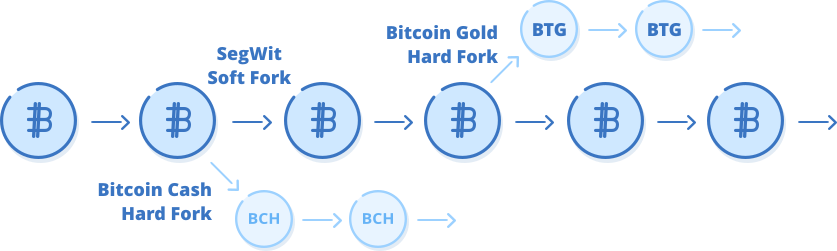
\includegraphics[width=\textwidth]{images/fig15.png}
    \caption{\footnotesize{\textit{Munten van een soft-fork kunnen naar oudere nodes gestuurd worden. Een hard-fork produceert nieuwe terugwaarts-incompatibele UTXO's die niet geaccepteerd zullen worden door oude nodes.}}}
    \label{fig15}
\end{figure}

Vele andere munten gebruiken vergelijkbare code, maar zijn begonnen met een lege blockchain zonder bitcoins transactiegeschiedenis. Voorbeelden hiervan zijn Litcoin en Dogecoin. Dergelijke munten zijn geen bitcoin forks omdat ze niet dezelfde transactiegeschiedenis delen, ookal zouden ze in code vergelijkbaar kunnen zijn. 

Een Bitcoinfork heeft geen enkel effect met betrekking tot de limiet van 21 miljoen Bitcoins. Vergelijk het met een wereld waarin de wereldwijde goudvoorraad ligt opgeslagen in het zwaarbewaakte en streng ontworpen Fort Knox. Nu bouw jij een klein en slecht ontworpen hutje, zet er een enkele bewaker voor en noemt het Fort Knox Lite. Je verft wat stenen met bladgoud en stopt ze in het hutje. Daaropvolgend breng je een nieuwsbericht uit om de wereld te vertellen dat je het goud hebt opgesplitst en iedere goudbezitter een equivalente hoeveelheid aan gratis stenen zult toekennen die opgeslagen liggen in je hutje. 

Bitcoin wordt inmiddels beveiligd door een groot aantal miners, waardoor een 51\% aanval vrijwel onbetaalbaar is geworden. Een fork van Bitcoin met slechts een handjevol miners is daarentegen ontzettend kwetsbaar. De code is waarschijnlijk gebrekkig en gebouwd door een onervaren team van ontwikkelaars, netzoals je hutje. De Bitcoin forks worden dan ook niet geaccepteerd door de bestaande nodes omdat ze breken met de regels van Bitcoin, netzoals iemand een steen met bladgoud ook niet zou accepteren. De productiekosten van de gesplitse munten en stenen zijn verwaarloosbaar, aangezien je ze gratis aan iedere bezitter hebt overhandigd. Daarmee wordt ook de marktinteresse al snel minder.

Nu je nadenkt over de duizenden Bitcoinklonen, allen zonder significante waarde, beschouw de volgende paradox: Bitcoin opsplitsen is eenvoudig en kost je niets. De regels van Bitcoin wijzigen of nieuwe bitcoin creëren is dat allesbehalve. Mocht iemand met beperkte Bitcoinkennis je vragen waarom Bitcoin speciaal is, dan weet je nu wat je kunt antwoorden.

De decentrale aard van het Bitcoin ecosysteem geeft grote voorkeur aan de status quo. Het implementeren van grote veranderingen neemt maanden of jaren in beslag aan het verkrijgen van consensus, discussie en peer review. Dit is van groot belang en wenselijk voor een systeem met als doel om als wereldwijd geld te fungeren. Bitcoin is een delicate dans tussen duizenden deelnemers die allemaal vanuit eigenbelang handelen, en vaak met tegengestelde belangen. Het is een volledig anarchisch vrije-markt systeem waar niemand de baas is. 

\chapter{What's next?}

\section{Is Bitcoin de MySpace van crypto?}

Waarom schrijf ik een boek over Bitcoin en niet over het grotere crypto ecosysteem? Zijn er geen duizenden andere munten? Wat maakt bitcoin zo speciaal, anders dan dat het de eerste decentrale cryptovaluta is? Is het niet trager dan andere munten en met minder mogelijkheden dan de nieuwe concurrenten?

Dit is een veelgestelde vraag van nieuwkomers. Na een eerste introductie tot bitcoin en haar werking, is de volgende logische vraag vaak: "Zo'n blockchain is interessant, maar hoe weten we dat er geen betere versie opdaagt die van bitcoin de MySpace maakt van crypto?"

Bitcoins concurrentievoordeel is veel, veel groter dan het voordeel destijds van MySpace. Laten we eens kijken wat een concurrent nodig heeft om bitcoin te vervangen.

\section{Gemakkelijker verkoopbaar en grotere liquiditeit}

Het eerste om te begrijpen is dat een vergelijking met MySpace en Facebook zwak is, omdat het je niets kost om tegelijkertijd op beide platforms een account te onderhouden. Dit is precies wat er gebeurde tijdens de transitie van de één naar de ander. Zodra genoeg kritieke massa was overgestapt naar Facebook, stopte men met MySpace.

Maar dit is niet hoe geld werkt. Als jij een euro aan bitcoin hebt, is dat een euro die je niet in een andere munt hebt. Je moet er bewust voor kiezen om de één voor de ander te verhandelen. Het is onmogelijk om tegelijkertijd hetzelfde vermogen op te slaan in verschillende munten. Vraag jezelf eens af: waarom zou je geld bewaren in iets anders dan de meest liquide en best geaccepteerde valuta. Het enige antwoord is speculatie. Als je niet in staat bent om de gehele economie te overtuigen om de andere munt te accepteren, dan is er geen enkele manier dat het dominant wordt. 

De liquiditeit van bitcoin is vele malen groter dan alle concurrenten. Op moment van schrijven is de marktkapitalisatie van bitcoin ongeveer \$1 biljard (1000 miljard).\footnote{\href{https://messari.io/onchainfx}{messari.io/onchainfx}} De eerstvolgende concurrent, Ethereum, heeft een kapitalisatie van slechts \$500 miljard. Dit zegt nog niets over de ware liquiditeit, de mate waarin je een aanzienlijk bedrag kunt verkopen zonder dat de prijs drastisch zal dalen. 

Liquiditeit heeft een sneeuwbaleffect. Het meeste liquide geld aanhouden, betekent dat andere mensen het willen, waardoor de liquiditeit nog verder toeneemt. Door vast te houden aan alles behalve het meest liquide geld, straf je jezelf in de hoop dat anderen hetzelfde gaan doen. Er is simpelweg geen enkele economisch motief om van de één op de andere dag massaal op een concurrent over te stappen.

\section{Aantoonbaar tien jaar \$1000 miljard beveiligd}

Bitcoin begon in 2009 als internet experiment voor computernerds. Slechts 1 jaar later volgde de eerste transactie (een pizza voor 10000 bitcoins) en inmiddels is 1 bitcoin al meer dan \$60.000 waard. Dit gebeurde in relatieve rust, zonder al te veel ophef. Door de jarenlange aanvallen is immuunsysteem van bitcoin inmiddels van wereldklasse, met het grootste netwerk aan rekenkracht ter wereld. Al tien jaar lang blijkt het onmogelijk om te hacken en het beveiligt inmiddels meer dan 1000 miljard dollar.

Het is haast onmogelijk om vandaag de dag in stilte een nieuwe cryptovaluta te lanceren. Laten we eens kijken naar een alternatieve blockchain, EOS, met een waarde van ongeveer ~\$10 miljard bij de lancering van het netwerk (en vandaag nog slechts de helft waard). Het netwerk moest slechts 2 dagen na aanvang al op slot wegens fouten in de code. Deze fouten werden zonder al te veel toezicht of review verholpen. Durf jij hier \$1000 miljard in bewaren? Misschien bestaat EOS over 10 jaar nog, wie het weet mag het zeggen. Maar tegen die tijd is bitcoin 20 jaar oud en beveiligt het biljarden aan waarde.  

\section{Aanvallen met bestaande rekenkracht afslaan}

Met duizenden crypto's en allerlei hashing-algoritmes, staat iedere nieuwe munt onder bedreiging van een 51\%-aanval met bestaande rekenkracht. Bitcoin Gold en vele andere munten zijn hier al slachtoffer van geweest.

Een nieuwe concurrent moet deze aanvallen van bestaande rekenkracht dus kunnen overleven, of moet op zoek naar een algoritme zonder gespecialiseerde ASIC's. Maar zonder ASIC's is het systeem juist weer kwetsbaar voor een aanval met standaard GPU's. Een ander probleem is dat een nieuwe concurrent niet zomaar vanaf dag 1 veel waarde kan beveiligen, zoals EOS probeerde. Dit is roekeloos en voorbode voor een gecentraliseerd systeem. Dat betekent dus ook dat een nieuwe concurrent niet zomaar geld op kan halen, maar net zoals bitcoin langzaam zal moeten groeien om de beveiliging proportioneel te laten groeien. Echter, met langzame groei wordt het haast onmogelijk om bitcoin nog in te halen. 

\section{Decentralisatie}

Een groot gedeelte van bitcoin's beveiligingsmodel berust op een hoge graad van decentralisatie. Dit betekent dat het moeilijk is om het protocol te wijzigen en men erop kan vertrouwen dat het de eigenschappen zoals beloofd in de broncode zal waarborgen (gelimiteerd aanbod, etc). Bitcoin bewees deze eigenschap te bezitten toen een groot aantal bedrijven en miners de blockgrootte wilden wijzigen, om het protocol een bepaalde richting op te sturen.\footnote{Lees hier meer over de achterkamertjespolitiek die plaatsvond bij de zogeheten Segwit2X fork:  \href{https://bitcoinmagazine.com/articles/now-segwit2x-hard-fork-has-really-failed-activate}{bitcoinmagazine.com/articles/now-segwit2x-hard-fork-has-really-failed-activate}}. De voorgestelde aanpassingen faalden spectaculair nadat ze werden afgewezen door de gebruikers van bitcoin. 

Een concurrent die decentralisatie nastreeft zal bedrijven en teams met bekende mensen moeten uitsluiten, om de onderdrukking en \textquotedbl{}single points of failure\textquotedbl{} te voorkomen. Ook munten met het motto \textquotedbl{}move fast and break things\textquotedbl{} zijn uitgesloten, want dat kan alleen bij voldoende centralisatie. Al met al is een concurrent dus snel en kwetsbaar voor centralisatie, of traag en niet in staat om bitcoin in te halen.

\section{Trek de beste ontwikkelaars aan}

Zoals de wervelwind van activiteit bij Linux, andere UNIX-achtige besturingssystemen weerhield van concurrentie, zo kan het ook gebeuren bij bitcoin. Elke dag wordt de gemeenschap groter en worden nieuwe bedrijven, met nieuwe diensten, gebouwd bovenop bitcoin. Een concurrent moet ontwikkelaars zien te stelen van een exponentieel groeiend netwerk, met inmiddels honderden bedrijven en tal van educatieve programma's en conferenties.  

\section{Een wereldwijd financieel netwerk}

Bitcoin wordt inmiddels gedragen door een wereldwijd netwerk van handelsbeurzen, futures en andere financiële derivaten bij grote spelers zoals de Chicago Mercantile Exchange (CME), honderden hefboomfonsen en handelskantoren, en een netwerk van mensen die bitcoin al gebruiken als alternatief voor gebroken valuta zoals de Venezulaanse bolivar. Bitcoin laat zich dus niet zo makkelijk vervangen.

Instellingen zoals de CME nemen een nieuwe concurrent pas op als er al voldoende handelsvolume is. Je zult bedrijven er dus van moeten overtuigen om de nieuwe concurrent te accepteren in plaat van bitcoin. Een concurrent die waarschijnlijk minder veilig en minder liquide is, minder competente ontwikkelaars heeft en per definitie over minder wereldwijde adoptie beschikt. 

\section{Solide geld}

Bitcoin is nooit bedoeld als snelle en goedkope manier van betalen. Dat is een groot misverstand. De fundamentele eigenschappen waarbij het grootboek wereldwijd wordt gerepliceerd, staan dat simpelweg niet toe. Daarentegen groeit bitcoin's primaire en reeds bewezen toepassing als censuur-resistent, solide geld. 

Alles wat daarbij komt, zoals het goedkoper maken van internationale overboekingen, zijn kersen op de taart. De meeste concurrenten richten zich nog steeds op snelle betalingen, terwijl dat probleem al redelijk goed is opgelost door vele gecentraliseerde bedrijven. Daarnaast heeft bitcoin daar ook inmiddels een oplossing voor gevonden met het snel groeiende Lightning Netwerk. 

Om te kunnen concurreren op het front van solide geld moeten onveranderbare eigenschappen en decentralisatie ten alle tijde voorop staan bij de ontwikkeling. Bitcoin's ecosysteem is gebouwd door \textit{cypherpunks} en heeft de kans gehad om langzaam te groeien, maar de meeste munten worden ontwikkeld door winstgedreven, gecentraliseerde teams en maken dus weinig kans op slagen.   

\newpage
\section{Toekomstige ontwikkelingen in Bitcoin}

We hebben inmiddels het volledige protocol onder de loep genomen. Laten we eens kijken naar de toekomst en sommige van de aankomende verbeteringen bespreken.

Bitcoin is programmeerbaar geld waar we allerlei diensten bovenop kunnen bouwen. Dit is een volledig nieuw concept en we staan pas aan het begin van wat mogelijk is.

\section{Lightning Netwerk}

Bitcoin heeft verschillende periodes van hoge transactievergoedingen gekend op momenten dat er hoge vraag was naar de blokruimte. Bitcoin is op dit moment slechts in staat om ongeveer 3 tot 7 transacties per seconde te verwerken, op basis van de hoeveelheid transacties die in een blok passen. Ook al kan een batch-transactie honderden mensen betalen in een transactie, dat is nog steeds te weinig capaciteit voor een wereldwijd betalingsnetwerk.    

Het vergroten van de blokruimte is een naïve oplossing en desondanks door veel concurrenten, waaronder Bitcoin Cash, toegepast. Bitcoin heeft gekozen voor een andere route omdat het vergroten van de blokken de decentrale eigenschappen zoals het aantal nodes en de geografische verspreiding van nodes negatief beïnvloedt. 

Een verhoging van de blokgrootte kan er hoe dan ook niet voor zorgen dat bitcoin geschikt wordt als wereldwijd betalingsnetwerk --- het schaalt simpelweg niet genoeg. Welkom bij het Lightning Netwerk: een protocol en verschillende software implementaties om \textit{off-chain} bitcointransacties te verwerken die periodiek kunnen verrekend worden op de blockchain. Over het Lightning Netwerk zouden we een heel boek kunnen schrijven, maar we beperken ons hier tot de hoofdlijnen.

De basisgedacht bij Lightning is dat we niet iedere transactie op de blockchain hoeven te registreren. Vergelijk het met een tijdelijke rekening bij de kroeg, waar drankjes worden aangestreept en pas aan het eind van de avond wordt afgerekend. Iedere drankje afzonderlijk betalen is tijdrovend en omslachtig. Voor bitcoin geldt min of meer hetzelfde: iedere koffie of ieder biertje registreren op de blockchain en die data verspreiden over duizenden computers over de wereld is niet schaalbaar, noch goed voor jouw privacy.

Het Lighting Netwerk heeft het potentieel om bitcoin op vele fronten te verbeteren:

\begin{itemize}
    \item Vrijwel ongelimiteerd transactievolume: honderdduizenden micro-transacties uitvoeren en eenmalig verrekenen op de blockchain. 
    
    \item Directe betaling: Wachten op confirmatie op de blokchain is niet langer nodig. 
    
    \item Extreem lage transactievergoedingen: geschikt voor micro-betalingen zoals de betaling van enkele centen om een blog te lezen. 
    
    \item Betere privacy: slechts de deelnemende partijen aan de transactie hebben er kennis van, in tegenstelling tot on-chain betalingen die met de hele wereld gedeeld worden.
    
\end{itemize}

Lightning maakt gebruik van betalingskanalen. Dit zijn on-chain bitcointransacties waarbij een hoeveelheid bitcoin wordt vastgezet en beschikbaar gemaakt binnen het Lightning Netwerk, voor directe, bijna kosteloze transacties. Het Lightning Netwerk is in de beginfase maar nu al veelbelovend. Zie als voorbeeld de website \href{https://yalls.org}{yalls.org} waar je via Lightning kunt betalen om artikelen te lezen.  

\section{Bitcoin in de ruimte}

Bitcoin is uitstekend bestand tegen censuur omdat het bestand is tegen aanvallen (je kan je eigendom in je hoofd bewaren), en bestand tegen censuur omdat er maar één eerlijke miner op het netwerk nodig is om jouw transacties uit te voeren (en je kunt zelf minen). 

Desalniettemin, aangezien bitcoin via internet wordt verstuurd is het vatbaar voor censuur op netwerkniveau. Bijvoorbeeld doordat autoritaire regimes die bitcoin willen onderdrukken, kunnen proberen om te verhinderen dat bitcoindata hun land binnenkomt en verlaat via het internet.

Het Blockstream Satellite-netwerk is een eerste poging om het netwerk uit te breiden en te beveiligen tegen censuur op staatsniveau, evenals een poging om afgelegen gebieden te bereiken die mogelijk geen verbinding met het internet hebben. Dit satellietsysteem maakt het voor iedereen met een schotel en relatief goedkope apparatuur, mogelijk om verbinding te maken en de bitcoin-blockchain te downloaden. Binnenkort wordt bidirectionele communicatie ook mogelijk. Er zijn nu ook inspanningen zoals TxTenna, die bouwen aan \textit{off-the-grid mesh-netwerken}. Als zo'n setup gecombineerd zou worden met een satellietverbinding, zou het bijna niet te stoppen zijn.

\backmatter

\chapter*{Verder lezen}

Dit was het. Je hebt bitcoin onder de loep genomen, en hopelijk ben je nu klaar om de wondere wereld van bitcoin verder te verkennen. Waar ga je heen vanaf hier? Hier zijn een paar bronnen om je verder te helpen:

\begin{itemize}
    \item \textit{De bitcoin standaard} (Saifedean Ammous) \href{https://konsensus.network/product/de-bitcoin-standaard/}{https://konsensus.network/product/de-bitcoin-standaard/}
    \item \textit{Bitcoin Investment Theses} (Pierre Rochard)
    \href{https://pierre-rochard.medium.com/bitcoin-investment-theses-part-1-e97670b5389b}{pierre-rochard.medium.com/bitcoin-investment-theses-part-1-e97670b5389b}
    \item \textit{Dank God voor Bitcoin/} (Lyle Pratt, George Mekhail, Jimmy Song, Gabe Higgins, Julia Tourianski, Derek Waltchack, Robert Breedlove en J.M. Bush) 
    \href{https://konsensus.network/product/dank-god-voor-bitcoin/}{konsensus.network/product/dank-god-voor-bitcoin/}
    \item \textit{Gelaagd Geld} (Nik Bahtia)
    \href{https://konsensus.network/product/gelaagd-geld/}{konsensus.network/product/gelaagd-geld/}
\end{itemize}

Om meer te lezen over de technische aspecten:

\begin{itemize}
    \item De whitepaper; \textit{Bitcoin: Een Peer-to-Peer Electronisch geld Systeem} (Satoshi Nakamoto) \href{https://bitcoin.org/files/bitcoin-paper/bitcoin\_nl.pdf}{bitcoin.org/files/bitcoin-paper/bitcoin\_nl.pdf}
    \item \textit{Mastering Bitcoin} (Andreas Antonopoulos)
    \item \textit{Programming Bitcoin} (Jimmy Song)
    \item Jimmy Songs seminar is beschikbaar op: \href{https://programmingblockchain.com}{programmingblockchain.com}
\end{itemize}

Achtergrondinformatie over de geschiedenis en filosofie van Bitcoin: 

\begin{itemize}
    \item \textit{Planting Bitcoin} (Dan Held)\\
    \href{https://medium.com/@danhedl/planting-bitcoin-sound-money-72e80e40ff62}{medium.com/@danhedl/planting-bitcoin-sound-money-72e80e40ff62}
    \item \textit{Bitcoin Governance} (Pierre Rochard)\\
    \href{https://medium.com/@pierre\_rochard/bitcoin-governance-37e86299470f}{medium.com/@pierre\_rochard/bitcoin-governance-37e86299470f}
    \item \textit{Bitcoin Past and Future} (Murad Mahmudov) \href{https://blog.usejournal.com/bitcoin-past-and-future-45d92b3180f1}{blog.usejournal.com/bitcoin-past-and-future-45d92b3180f1}
    \item De video's van Andreas Antonopoulos video's, en in het bijzonder \textit{Currency Wars} en \textit{The Monument of Immutability}, \href{https://www.youtube.com/user/aantonop}{youtube.com/user/aantonop}
\end{itemize}

Een groot deel van het bitcoin-ecosysteem leeft op Twitter. Hier is een lijst van mensen in willekeurige volgorde, die de moeite waard zijn om te volgen. Begin hier en ga dieper het konijnenhol in:

\newpage

\noindent\href{https://twitter.com/lopp}{@lopp}
\\\noindent\href{https://twitter.com/pwuille}{@pwuille}
\\\noindent\href{https://twitter.com/adam3us}{@adam3us}
\\\noindent\href{https://twitter.com/danheld}{@danheld}
\\\noindent\href{https://twitter.com/pierre\_rochard}{@pierre\_rochard}
\\\noindent\href{https://twitter.com/bitstein}{@bitstein}
\\\noindent\href{https://twitter.com/theonevortex}{@theonevortex}
\\\noindent\href{https://twitter.com/AlenaSatoshi}{@AlenaSatoshi}
\\\noindent\href{https://twitter.com/WhatBitcoinDid}{@WhatBitcoinDid}
\\\noindent\href{https://twitter.com/stephanlivera}{@stephanlivera}
\\\noindent\href{https://twitter.com/TheBlock\_\_}{@TheBlock\_\_}
\\\noindent\href{https://twitter.com/TheLTBNetwork}{@TheLTBNetwork}
\\\noindent\href{https://twitter.com/real\_vijay}{@real\_vijay}
\\\noindent\href{https://twitter.com/jimmysong}{@jimmysong}
\\\noindent\href{https://twitter.com/Excellion}{@Excellion}
\\\noindent\href{https://twitter.com/starkness}{@starkness}
\\\noindent\href{https://twitter.com/dickerson\_des}{@dickerson\_des}
\\\noindent\href{https://twitter.com/roasbeef}{@roasbeef}
\\\noindent\href{https://twitter.com/saifedean}{@saifedean}
\\\noindent\href{https://twitter.com/Melt\_Dem}{@Melt\_Dem}
\\\noindent\href{https://twitter.com/\_jillruth}{@\_jillruth}
\\\noindent\href{https://twitter.com/giacomozucco}{@giacomozucco}
\\\noindent\href{https://twitter.com/Snyke}{@Snyke}
\\\noindent\href{https://twitter.com/aantonop}{@aantonop}
\\\noindent\href{https://twitter.com/MustStopMurad}{@MustStopMurad}
\\\noindent\href{https://twitter.com/danheld}{@danheld}
\\\noindent\href{https://twitter.com/peterktodd}{@peterktodd}
\\\noindent\href{https://twitter.com/dergigi}{@dergigi}
\\\noindent\href{https://twitter.com/skwp}{@skwp}
\\\noindent\href{https://twitter.com/konsensusn}{@KonsensusN}
\paragraph{}


Je kunt meer van mijn geschriften vinden op  \href{https://yanpritzker.com}{yanpritzker.com}.

\noindent \hspace{-0.5\baselineskip} Tot ziens aan de andere kant.


\chapter*{Dankwoord}

\vspace{-3\baselineskip}

Ik wil graag mijn dank uitspreken richting de vele mensen die me feedback hebben gegeven tijdens de vroege concepten van dit boek. In het bijzonder: Joe Levering, Phil Geiger, Yury Pritzker, Jonathan Wheeler, Walter Rosenberg, Michael Santosuosso en David Harding. Ook wil ik Jimmy Song bedanken voor het Programming Blockchain-seminar, waaardoor ik de schop onder mijn kont kreeg die ik nodig had om dit boek te schrijven.

\chapter*{Over de auteur}

Yan Pritzker is al 20 jaar ontwikkelaar en ondernemer, met veel ervaring in het opstarten van bedrijven. Yan is mede-oprichter en CTO van Swan Bitcoin, een bedrijf dat zich richt op educatie en begeleiding van de volgende tien miljoen (nieuwe) bitcoiners.
Yan schrijft over bitcoin en aanverwante onderwerpen op \href{https://yanpritzker.com}{yanpritzker.com}. Je kunt hem ook volgen op Twitter: \href{https://twitter.com/skwp}{@skwp}.


\end{document}
% END THE DOCUMENT